\chapter{\acsp{LSDDM} design with Response Surface Modelling}   \label{Chapter:PMLSM design RSM}


    The concept of a “metamodel” is introduced as a reasonably accurate surrogate model, constructed via \acf{RSM} and powered by reduced-order models, deep neural networks, or statistically derived models. This chapter aims toward providing and applying an end-to-end \acs{RSM} design process that is viable for selected motor topologies: \acf{PMLSM}, \acf{LFSM}, and \acf{LTFM}. This process should be both specific and flexible enough to make a fair comparison between these types of motors in \acs{NFJI} applications. In order to achieve this goal, Section\,\ref{Chapter:RSM/outline} thoroughly investigates the \acs{RSM} method to establish a suitable design process. Then, Sections\,\ref{Chapter:RSM/PMLSM}, \ref{Chapter:RSM/LFSM}, and \ref{Chapter:RSM/LTFM} look at applying the established process for the selected types of motors. The optimization problem statement, the objective function and the high-level constraints for each motor topology explored in this chapter are equivalent to the optimization problem already established in Section\,\ref{Chapter:PMLSM design HM/design optimization/optimization formulation/out} and Equation\,\ref{eq:outer optimization for PMLSMs}. By comparing optimization results for \acsp{PMLSM} obtained in Section\,\ref{Chapter:PMLSM design HM/design optimization/results} and Section\,\ref{Chapter:RSM/PMLSM}, a fair indicator for the accuracy and correctness of the \ac{RSM} method is gathered. Toward the end of this chapter, Section\,\ref{Chapter:RSM/discussion} aggregates the results collected in the previous optimization runs of different types of motors in order to choose the most suitable type of linear synchronous motor for \acs{NFJI} application.


    % ===================================================================================================
    % === NEW SECTION === NEW SECTION === NEW SECTION === NEW SECTION === NEW SECTION === NEW SECTION ===
    % ===================================================================================================
    \section{Process outline}                        \label{Chapter:RSM/outline}
    
    
        \acf{DOE} together with \ac{RSM} have been applied to many engineering problems. These studies often include statistical processes to investigate how the input correlates to the output, and which inputs have the greatest effect on the outputs. In applications where the cost of acquiring an actual input and output pair is expensive, \ac{DOE} sampling methods are helpful in reducing the data acquisition cost. 
        
        
        \ac{DOE} sampling methods can be divided into two classes: Factorial designs and Taguchi methods. Factorial designs include a full factorial, where all possible combinations of the factor levels are investigated, or only part of the full factorial are selected for acquisition. A full factorial is very useful because it allows the data analyst to observe the effects of changing the factor by providing all the available data interactions. It is recommended to use full factorial when possible. On the other hand, fractional factorial designs reduce the accuracy of the analysis in exchange for a lower data acquisition cost. In reality, an experiment can have full factorials for some inputs and fractional factorials for less important inputs. Taguchi methods use orthogonal arrays to gain detailed information about effects of factors with the minimum number of experiments. As a result, Taguchi methods, with fewer simulations, provide an important cost advantage to factorial designs. 
        
        
        In a high order \ac{RSM} problems with many input variables, reaching a large sampling levels set for each input is the key to producing accurate model predictions. However, the time and computation effort required to reach the high sampling levels grow exponentially with the number of input parameters. Only when the data acquisition budget allows, obtaining an extra set of data based on a set of randomly generated input sets will be helpful in increasing the "metamodel" accuracy. In this body of work, the method of constructing and inferring deep regression \acf{ANN} is employed to train the most accurate and generalized models that could be achieved.
        
        
        All types of motor topology studies in this chapter follow the common design criteria established in Section\,\ref{Chapter:PMLSM design HM/design optimization/design citeria}. The overall \ac{RSM} process to be applied widely in this chapter is outlined as follow:
        
        
        \begin{itemize}
            \item RSM problem statement - starting from topology, this step defines and selects the design parameters, value ranges and sampling level of the parameters,
            \item Data mining - constructs the experiment with the sampling levels previously obtained, then acquire the training data via a selected computational method (be it Harmonic Modelling or Finite Element Analysis) for a single repeating unit,
            \item Model fitting - trains/fits the training data into an \ac{ANN} that best represents the motor topology at hand in the range of values already specified,
            \item Optimization - performs convex non-linear optimization that utilizes the \ac{ANN} model trained earlier.
        \end{itemize}
        

    % ===================================================================================================
    % === NEW SECTION === NEW SECTION === NEW SECTION === NEW SECTION === NEW SECTION === NEW SECTION ===
    % ===================================================================================================
    \section{Application to PMLSM}             \label{Chapter:RSM/PMLSM}
    
        
        In this section, the aim of the work is to examine the effectiveness of the proposed design process by comparing optimization results obtained by the \acs{HM} method, to the optimization results obtained by the \acs{RSM} method. Fig.\,\ref{fig:chapter/rsm/PMLSM optimization} illustrates the \acs{RSM} design process adapted to the \acs{PMLSM} topology already presented in \ref{Chapter:PMLSM design HM/electromagnetic model/topology}. 
        
        
        \begin{figure*}[h]
            \centering
            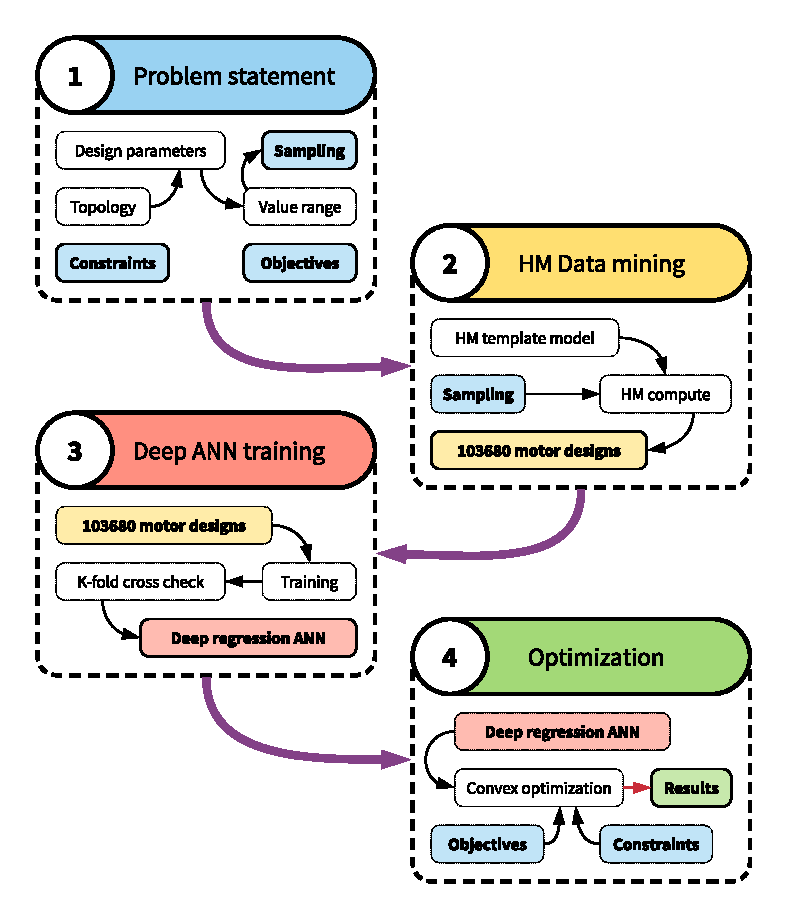
\includegraphics[width=4.5in]{chap4/images/optimization_process_RSM_for_PMLSM.pdf}
            \caption{Flowchart of the RSM motor design process adapted for PMLSM.}
            \label{fig:chapter/rsm/PMLSM optimization}
        \end{figure*}
        
        
        % -----------------------------------------------------------------------------------
        % --- NEW SUB SECTION --- NEW SUB SECTION --- NEW SUB SECTION --- NEW SUB SECTION --- 
        % -----------------------------------------------------------------------------------
        \subsection{Specifications \& Samplings}    \label{Chapter:RSM/PMLSM/spec}
        
        
            Re-using the considerations of the \acs{PMLSM} topology already presented in Section\,\ref{Chapter:PMLSM design HM/electromagnetic model/topology}, this work refers back to the design parameters $t_c$, $t_m$, $r_{mi}$, $L_k$, $\delta$ and their accompanying value ranges listed in Table\,\ref{table:table_of_optimization_constraints_PMLSM}. Additionally, the magnet to coil gap $gap_{mc}$ and coil to iron gap $gap_{cf}$ are addressed as constant values. 
            
            
            Table.\,\ref{table:RSM design level for PMLSM} shows incremental sampling steps for the structural design factors. From the sampling steps, a full factorial design grid of $51840$ designs was generated. Additionally, the same number of design cases were constructed by random input variables in the ranges specified by Table\,\ref{table:RSM design level for PMLSM}. The purpose of combining the factorial design space and the randomly generated design cases is to help generalize the supposedly continuous \acs{RSM} response better. In total, there were $103680$ independent motor designs available for \acs{ANN} training. To maximize the re-usability of the data collected, the obvious choice is to use \acs{HM} to generate a library of design for motors with only a single repeating unit. All of these motor designs were assumed to have the number of half coil periods $N_C$ and the number of half magnet periods $N_M$ of $1$. The input power was also to be kept at $P=1500\mathrm{W}$, in order to directly compare with the study in Chapter\,\ref{Chapter:PMLSM design HM}.
            
            
            \begin{table}[!h]
                \renewcommand{\arraystretch}{1.2}
                \caption{Summary of motor parameter sampling levels for \acs{RSM} of \acs{PMLSM}}
                \label{table:RSM design level for PMLSM}
                \centering
                \begin{tabular}{@{}l r r r r r r r@{}}
                \hline
                \bfseries Params & \bfseries Level 1 & \bfseries Jump step & \bfseries Last level & \bfseries Unit \\
                \hline
                    $L_k$       &   18     &   2     &   90     &   $\mathrm{mm}$\\
                    $r_{mi}$    &    2     &   2     &   10     &   $\mathrm{mm}$\\
                    $t_m$       &    2     &   2     &   20     &   $\mathrm{mm}$\\
                    $t_c$       &    3     &   2     &   19     &   $\mathrm{mm}$\\
                    $\delta$    &  0.1     & 0.1     &  0.6     &   \\
                \hline
                \end{tabular}
            \end{table}
        
        
        % -----------------------------------------------------------------------------------
        % --- NEW SUB SECTION --- NEW SUB SECTION --- NEW SUB SECTION --- NEW SUB SECTION --- 
        % -----------------------------------------------------------------------------------
        \subsection{HM data mining}           \label{Chapter:RSM/PMLSM/data mining}
        
        
            The base \acs{HM} computation model in Section\,\ref{Chapter:PMLSM design HM/electromagnetic model/hm solution} was re-purposed to help generate motor design data. To facilitate for the data mining and the optimization process later on, the same electromagnetic model was converted into a re-usable function as illustrated in Fig.\,\ref{fig:chapter/rsm/PMLSM/mining process}. The free inputs included the repeat length $L_k$, the inner radius of the cylindrical magnet array $r_{mi}$, the magnet radial thickness $t_m$, the coil radial thickness $t_c$, and the proportion of the radially magnetized magnet against the total length of the magnet. The fixed input included the number of half coil-phase $N_C$, the number of half magnet-phase $N_M$, and the power $P$. On the output side, the data mining function provided the half repeating unit mass $M$, motor constant $K_m$ and the linear force produced $F$.
        
        
            \begin{figure}
                \centering
                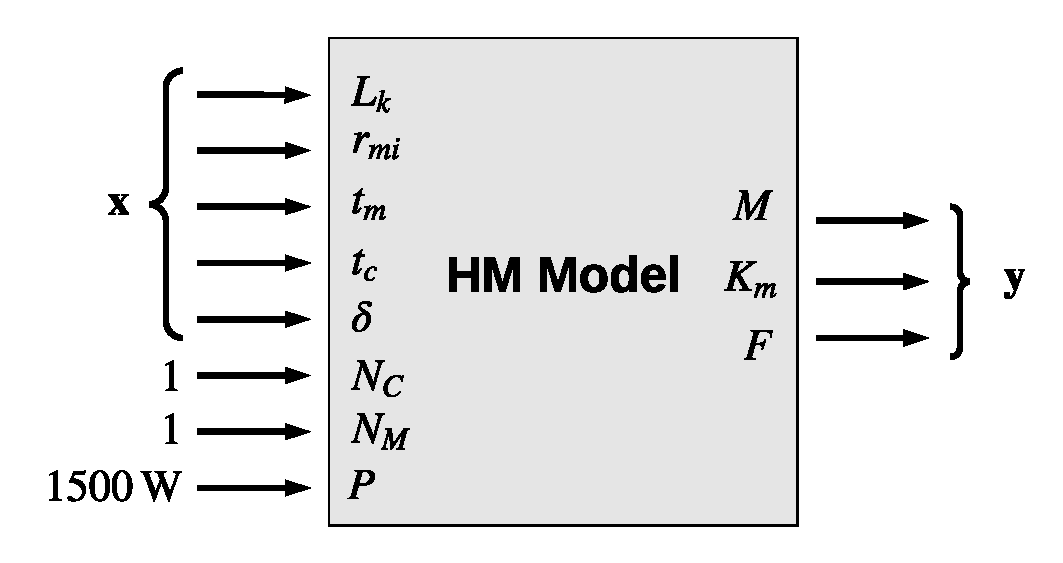
\includegraphics[width=4in]{chap4/images/HM_mining_for_PMLSM.pdf}
                \caption{A re-usable function to obtain RSM training data based on HM calculations of PMLSM.}
                \label{fig:chapter/rsm/PMLSM/mining process}
            \end{figure}
            
            
            The $103680$ input cases were queried against a re-usable function as illustrated in Fig.\,\ref{fig:chapter/rsm/PMLSM/mining process} to obtain the corresponding outputs for each input set. The necessary information was then reduced back to a table that captured the motor design parameters in CSV format. 
            
        
        % -----------------------------------------------------------------------------------
        % --- NEW SUB SECTION --- NEW SUB SECTION --- NEW SUB SECTION --- NEW SUB SECTION --- 
        % -----------------------------------------------------------------------------------
        \subsection{Deep regression ANN training}   \label{Chapter:RSM/PMLSM/ANN training}
        
            
            Deep learning belongs to a broader family of machine learning methods which is very useful in capturing complex non-linear patterns with almost any data set. The data set is required to provide both the continuous input variables (structural design factors), and the continuous output variable (thrust characteristics at a given power). The classification of this application is a supervised and regression type of machine learning problem.
            
            
            Because some design parameters ($gap_{mc}$, $gap_{cf}$, $P$ and others) were established with constant values, the \acs{ANN} do not need to include them into the Input Layer. On the other hand, including both the thrust $F$ and the motor constant $K_m$ will introduce unwanted redundancy for a fixed power $P$ study. Therefore, only the motor constant $K_m$ was included in the model prediction. Three \acs{ANN} models were implemented and trained using Keras and Tensorflow machine learning frameworks:
            
            
            \begin{itemize}
                \item $5$ structural parameters were regarded as the Input Layer: $L_k$,$r_{mi}$, $t_m$, $t_c$, and $\delta$,
                \item $1$ performance output was regarded as the Output Layer: $K_m$,
                \item The optimizer for training the \acs{ANN} was the Adam optimizer\,\cite{Kingma2014},
                \item $6$ hidden layers of densely connected nodes: $256-512-512-512-512-512$ nodes for each layer,
                \item The rectified linear unit (ReLU) activation function was used
for the input and hidden layer,
                \item The linear activation function was used for the output layer,
                \item The error to optimize for was \acf{MSE},
                \item The training and validation split chosen at random for each of the three models were: $70\%-30\%$, $75\%-25\%$, and $80\%-20\%$,
                The final \acs{ANN} model was ensembled from the average of three models above.
            \end{itemize}
            
            
            \begin{figure*}[!ht]
                \centering
                \subfloat[$70\%-30\%$ split model
                ]{
                    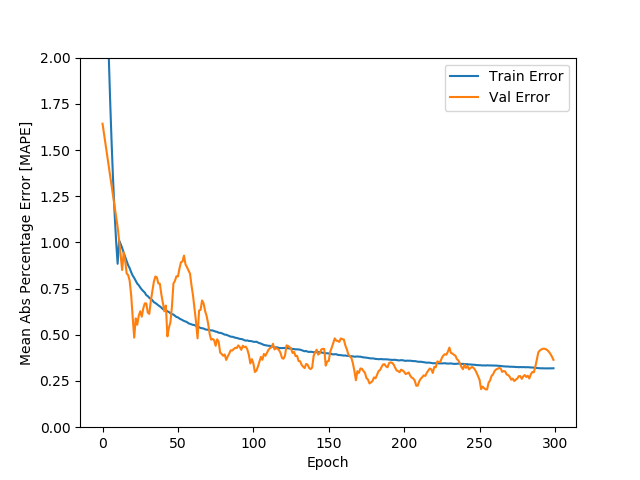
\includegraphics[width=0.5\textwidth]{chap4/images/MAPE_MSE_6_70-30_SPLIT.png}
                    \label{fig:chapter/rsm/PMLSM/training result/MAPE_70_30}
                }
                \subfloat[$75\%-25\%$ split model
                ]{
                    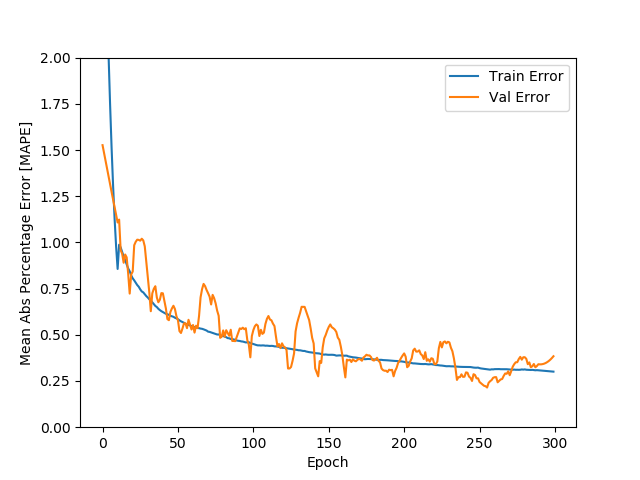
\includegraphics[width=0.5\textwidth]{chap4/images/MAPE_MSE_6_75-25_SPLIT.png}
                    \label{fig:chapter/rsm/PMLSM/training result/MAPE_75_25}
                }
                \\
                \subfloat[$80\%-20\%$ split model
                ]{
                    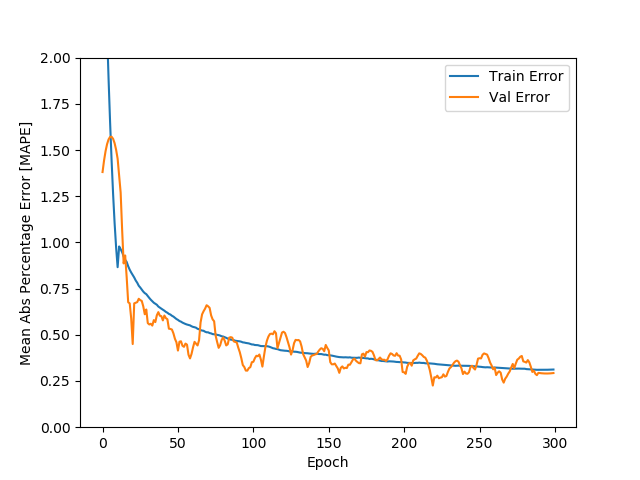
\includegraphics[width=0.5\textwidth]{chap4/images/MAPE_MSE_6_80-20_SPLIT.png}
                    \label{fig:chapter/rsm/PMLSM/training result/MAPE_80_20}
                }
                \caption{
                    Error produced by the deep learning \acs{ANN} model to represent \acsp{PMLSM}  vs. iterations for the training data (blue) and validation data (orange). The \acs{MAPE} is plotted for the training process of (a) $70\%-30\%$, (b) $75\%-25\%$, and (c) $80\%-20\%$ models, respectively.
                }   \label{fig:chapter/rsm/PMLSM/training result}
            \end{figure*}
            
            
            After $300$ training iterations, the models were shown to have an average \acf{MAPE} of $0.24\%$. The training and validation errors were similar, showing that the deep regression model was not over-fitted to the training data set. Fig.\,\ref{fig:chapter/rsm/PMLSM/training result} shows the training and validation error during the \acs{ANN} training process for each of the three models studied.
            
        
        % -----------------------------------------------------------------------------------
        % --- NEW SUB SECTION --- NEW SUB SECTION --- NEW SUB SECTION --- NEW SUB SECTION --- 
        % -----------------------------------------------------------------------------------
        \subsection{Optimization}                   \label{Chapter:RSM/PMLSM/Optimization}
        
        
            Following the outer and inner optimization setup in Section\,\ref{Chapter:PMLSM design HM/design optimization/optimization formulation}, the next step was to repeat the optimization run in Section\,\ref{Chapter:PMLSM design HM/benchmark study} with some differences. Instead of using the \acs{HM} equations as the mean estimate $K_m$ for the whole motor, the \acs{ANN} was employed to estimate the motor constant $K_m$ of a single repeat unit consisting of one half coil-phase ($N_C = 1$), and one half magnet-phase ($N_M = 1$). 
            
            
            During the execution of the optimization algorithm, many motors with half coil-phase values larger than $N_C = 1$ were calculated. As mentioned previously, the \acs{ANN} only estimate $K_m$ for motor units with $N_C=1$ and $N_M=1$. There requires a conversion for the motor constant of the whole motor $K_{m-whole}$, given that a new number of half coil-phase $N_{C-whole}$ that is larger than $1$:
            
            
            \begin{equation}
                K_{m-whole}=K_m  \sqrt{N_{C-whole}}
                \label{eq:calculate new K_m based on new N_C}
            \end{equation}
            
            
            Adapting to this change, the maximum jet velocity $v_{jet}$ becomes:
            
            
            \begin{equation}
                v_{jet} = \sqrt[4]{\frac{4P {K_{m-whole}}^2 {L_S}^2}{\rho_w V^2}}
                \label{eq:calculate new v_jet based on new N_C}
            \end{equation}
            
            
            Except when it comes to collecting the motor mass $M$, Equation\,\ref{eq:mass of motor via mass dimless} was borrowed from the \acs{HM} electromagnetic calculation. 
            
            
            \begin{figure*}[!ht]
                \par\bigskip
                \centering
                \subfloat[Sub-routine setup: Each objective function evaluation will start a separate sub-routine, taking roughly $6$ seconds.]{
                    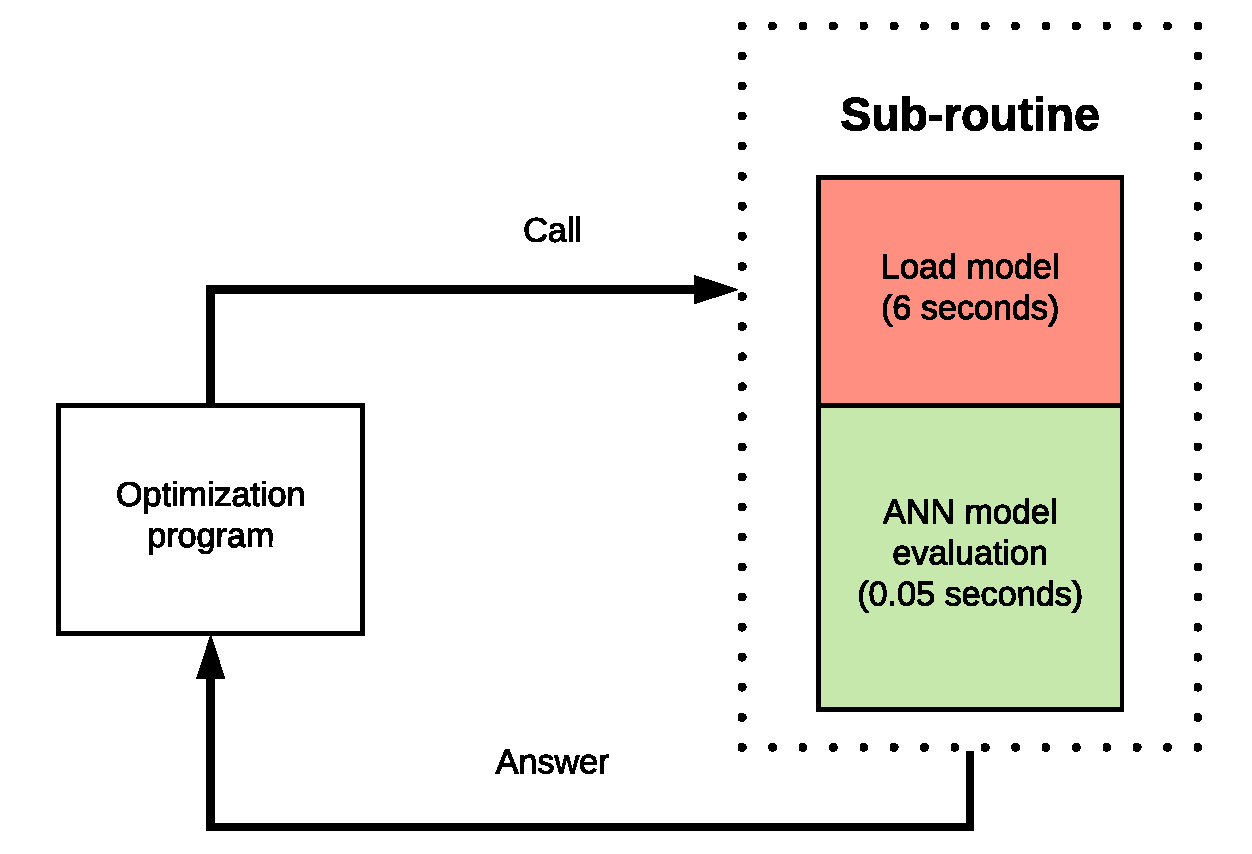
\includegraphics[width=0.45\textwidth]{chap4/images/inference_routine.pdf}
                    \label{fig:chapter/rsm/PMLSM/inference options/routine}
                }
                \,\,\,\,\,\,
                \subfloat[Web-server setup: The model is loaded only once, and all objective function evaluations take less than $0.05$ seconds.]{
                    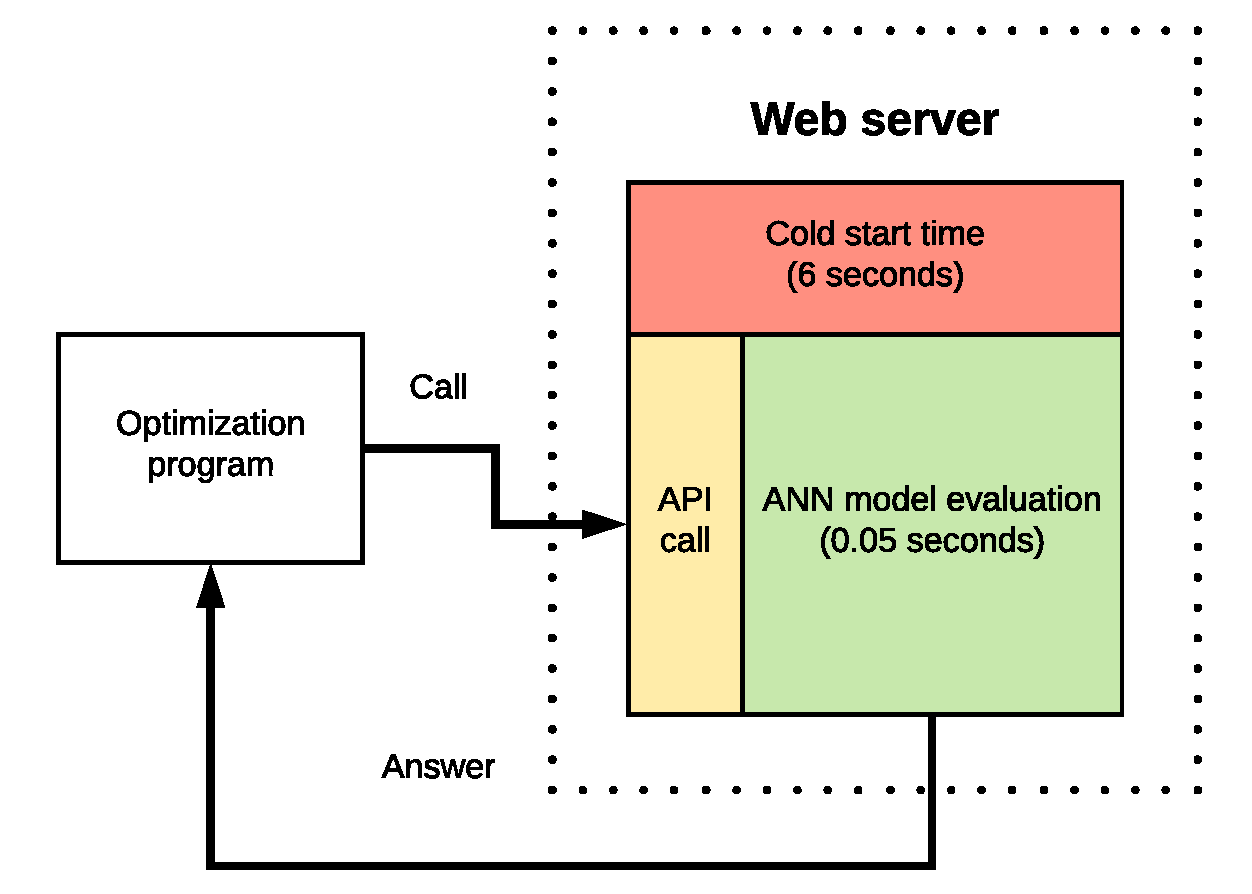
\includegraphics[width=0.45\textwidth]{chap4/images/inference_web_services.pdf}
                    \label{fig:chapter/rsm/PMLSM/inference options/web services}
                }
                \caption{
                    Two different styles of optimization objective function evaluation.
                }\label{fig:chapter/rsm/PMLSM/inference options}
            \end{figure*}
            
            
            In the normal circumstances, a full execution cycle for inferring the \acs{ANN} model includes waiting for the model to load, querying the model, then terminating the model until the next execution. However, loading the \acs{ANN} model in the Python environment may take a few seconds, the result is that numerous inferences of the existing model made by the optimization algorithm would cost an enormous amount of time. Alternatively, the optimization objective function evaluation should interact with the trained \acs{ANN} model in the fashion of a web server instead of a sub-routine, as illustrated in Fig.\,\ref{fig:chapter/rsm/PMLSM/inference options}.


        % -----------------------------------------------------------------------------------
        % --- NEW SUB SECTION --- NEW SUB SECTION --- NEW SUB SECTION --- NEW SUB SECTION --- 
        % -----------------------------------------------------------------------------------
        \subsection{Results}                   \label{Chapter:RSM/PMLSM/Results}


            With the objective function evaluation using \acs{ANN} models at its core, the global optimization of \acs{PMLSM} for the problem described in Equation\,\ref{eq:outer optimization for PMLSMs} is summarized in Table\,\ref{table:result for global optimization of PMLSM via RSM method}. The table shows the optimization results for different motor mass constraints $M_0=[325,350,375,400,425]\,\mathrm{g}$.
            
            
            For instance, the global optimization for the constraints set $P=1500\,\mathrm{W}$, $V=1\,\mathrm{mL}$, $gap_{mc}=1.2\,\mathrm{mm}$, $gap_{cf}=0.1\,\mathrm{mm}$, $M_0=325\,\mathrm{g}$ on the search space of $L_{M0}:120\,\mathrm{mm}\rightarrow 160\,\mathrm{mm} \times L_{C0}:50\,\mathrm{mm}\rightarrow 90\,\mathrm{mm}$, the optimization program found an under-hung motor with $N_C=4$, $N_M=12$, $L_k=26.5\,\mathrm{mm}$, $r_{mi}=2\,\mathrm{mm}$, $t_m=6.15\,\mathrm{mm}$, $t_c=3\,\mathrm{mm}$, $\delta=0.30$. This motor configuration is able to theoretically produce $246.45\,\mathrm{N}$ at the rated power, which corresponds to a motor constant $K_m=6.36\,\mathrm{N/\sqrt{W}}$ and a peak jet speed $v_{jet}=228.67\,\mathrm{m/s}$. Table\,\ref{table:result for global optimization of PMLSM via HM method} shows that the same optimization problem powered by \acs{HM} electromagnetic equations produced almost exactly the same results when compared with \acs{RSM} method. The \acs{RSM} method predicted the peak jet speed $v_{jet}=228.67\,\mathrm{mm}$ while the \acs{HM} method predicted $v_{jet}=228.92\,\mathrm{mm}$. The only difference was the value of the ratio $\delta$ which does not affect the motor mass $M$.  
            
            
            Fig.\,\ref{fig:chapter/rsm/PMLSM/results} provides global optimization plots of $v_{jet}$ for the search space $L_{M0}:120\,\mathrm{mm}\rightarrow 160\,\mathrm{mm} \times L_{C0}:50\,\mathrm{mm}\rightarrow 90\,\mathrm{mm}$ using $P=1500\,\mathrm{W}$, $V=1\,\mathrm{mL}$, $gap_{mc}=1.2\,\mathrm{mm}$, $gap_{cf}=0.1\,\mathrm{mm}$,  and $M_0=[325,350,375,400,425]\,\mathrm{g}$. Not only do the global optimization results obtained by different modelling methods agreed strongly, the contour plots populated by the optimization processes of \acs{RSM} (Fig.\,\ref{fig:chapter/rsm/PMLSM/results}) and \acs{HM} (Fig.\,\ref{fig:chapter/hm/optimization search space result for differnt mass}) looked almost identical. This study successfully demonstrated the effectiveness and the accuracy of design and optimization process presented in Section\,\ref{Chapter:RSM/outline}.
        

            
            \begin{landscape}
                \begin{table}
                    \renewcommand{\arraystretch}{1.2}
                    \caption{Summary of motor design optimization values and performance using \acs{RSM} method}
                    \label{table:result for global optimization of PMLSM via RSM method}
                    \centering
                    \begin{tabular}{lllrrrrr}
                        \hline
                        \textbf{Params}     & \textbf{Description}                            & \textbf{Unit}           & $M_0=\mathbf{325\,g}$ & $\mathbf{350\,g}$ & $\mathbf{375\,g}$ & $\mathbf{400\,g}$ & $\mathbf{425\,g}$ \\
                        \hline
                        $P$        & Power dissipation in coil winding      & $\mathrm{kW}$  & $1.50$                & $1.50$            & $1.50$            & $1.50$            & $1.50$            \\
                        $V$        & Volume of ampoule                      & $\mathrm{mL}$  & $1.00$                & $1.00$            & $1.00$            & $1.00$            & $1.00$            \\
                        $gap_{mc}$ & Magnet and coil fixed gap              & $\mathrm{mm}$  & $1.20$                & $1.20$            & $1.20$            & $1.20$            & $1.20$            \\
                        $gap_{cf}$ & Coil and iron fixed gap                & $\mathrm{mm}$  & $0.10$                & $0.10$            & $0.10$            & $0.10$            & $0.10$            \\
                        \hline
                        $L_{C0:optim}$ & Constraint $L_C$ winding at global optimum & $\mathrm{mm}$        & $53.00$                       & $53.00$           & $53.00$           & $53.00$           & $53.00$           \\
                        $L_{M0:optim}$ & Constraint $L_C+L_S$ at global optimum        & $\mathrm{mm}$        & $160.00$                      & $160.00$          & $160.00$          & $160.00$          & $160.00$          \\
                        \hline
                        $r_{mi}$   & Magnet array inner radius              & $\mathrm{mm}$  & $2.00$                & $2.00$            & $2.00$            & $2.00$            & $2.00$            \\
                        $t_m$      & Magnet thickness                       & $\mathrm{mm}$  & $6.15$                & $6.35$            & $6.67$            & $6.99$            & $7.29$            \\
                        $t_c$      & Coil thickness                         & $\mathrm{mm}$  & $3.00$                & $3.00$            & $3.00$            & $3.00$            & $3.00$            \\
                        $\delta$   & Ratio of radial magnet vs. magnet pair &                & $0.32$                & $0.25$            & $0.25$            & $0.25$            & $0.27$            \\
                        $N_C$      & Number of half coil-poles              &                & $4$                   & $3$               & $3$               & $3$               & $3$               \\
                        $N_M$      & Number of half magnet-poles            &                & $12$                  & $9$               & $9$               & $9$               & $9$               \\
                        \hline
                        $t_f$      & Iron shell thickness                   & $\mathrm{mm}$  & $0.77$                        & $1.07$            & $1.12$            & $1.15$            & $1.19$    \\       
                        $L_k$      & Full pole length                       & $\mathrm{mm}$  & $26.50$               & $35.33$           & $35.33$           & $35.33$           & $35.33$           \\
                        $L_C$      & Length of coil array                   & $\mathrm{mm}$  & $53.00$               & $53.00$           & $53.00$           & $53.00$           & $53.00$           \\
                        $L_M$      & Length of magnet array                 & $\mathrm{mm}$  & $159.00$              & $159.00$          & $159.00$          & $159.00$          & $159.00$          \\
                        $L_S$      & Stroke length                          & $\mathrm{mm}$  & $106.00$              & $106.00$          & $106.00$          & $106.00$          & $106.00$          \\
                        \hline
                        $v_{jet}$  & Achievable jet speed                   & $\mathrm{m/s}$ & $228.64$              & $234.21$          & $239.81$          & $245.13$          & $250.10$         \\
                        $F$        & Force exerts on piston                 & $\mathrm{N}$         & $246.45$                      & $258.72$          & $271.35$          & $283.44$          & $295.06$          \\
                        $K_m$      & Motor constant                         & $\mathrm{N/\sqrt{W}}$ & $6.36$                        & $6.68$            & $7.01$            & $7.32$            & $7.62$           \\
                        \hline
                    \end{tabular}
                \end{table}
            \end{landscape}
            
            \begin{figure*}[!ht]
                \centering
                \subfloat[$M_0=325\,\mathrm{g}$. Global optimum found at $L_{C0}=53\,\mathrm{mm}$, $L_{C0}=160\,\mathrm{mm}$, $N_C=4$, and $N_M=12$.
                ]{
                    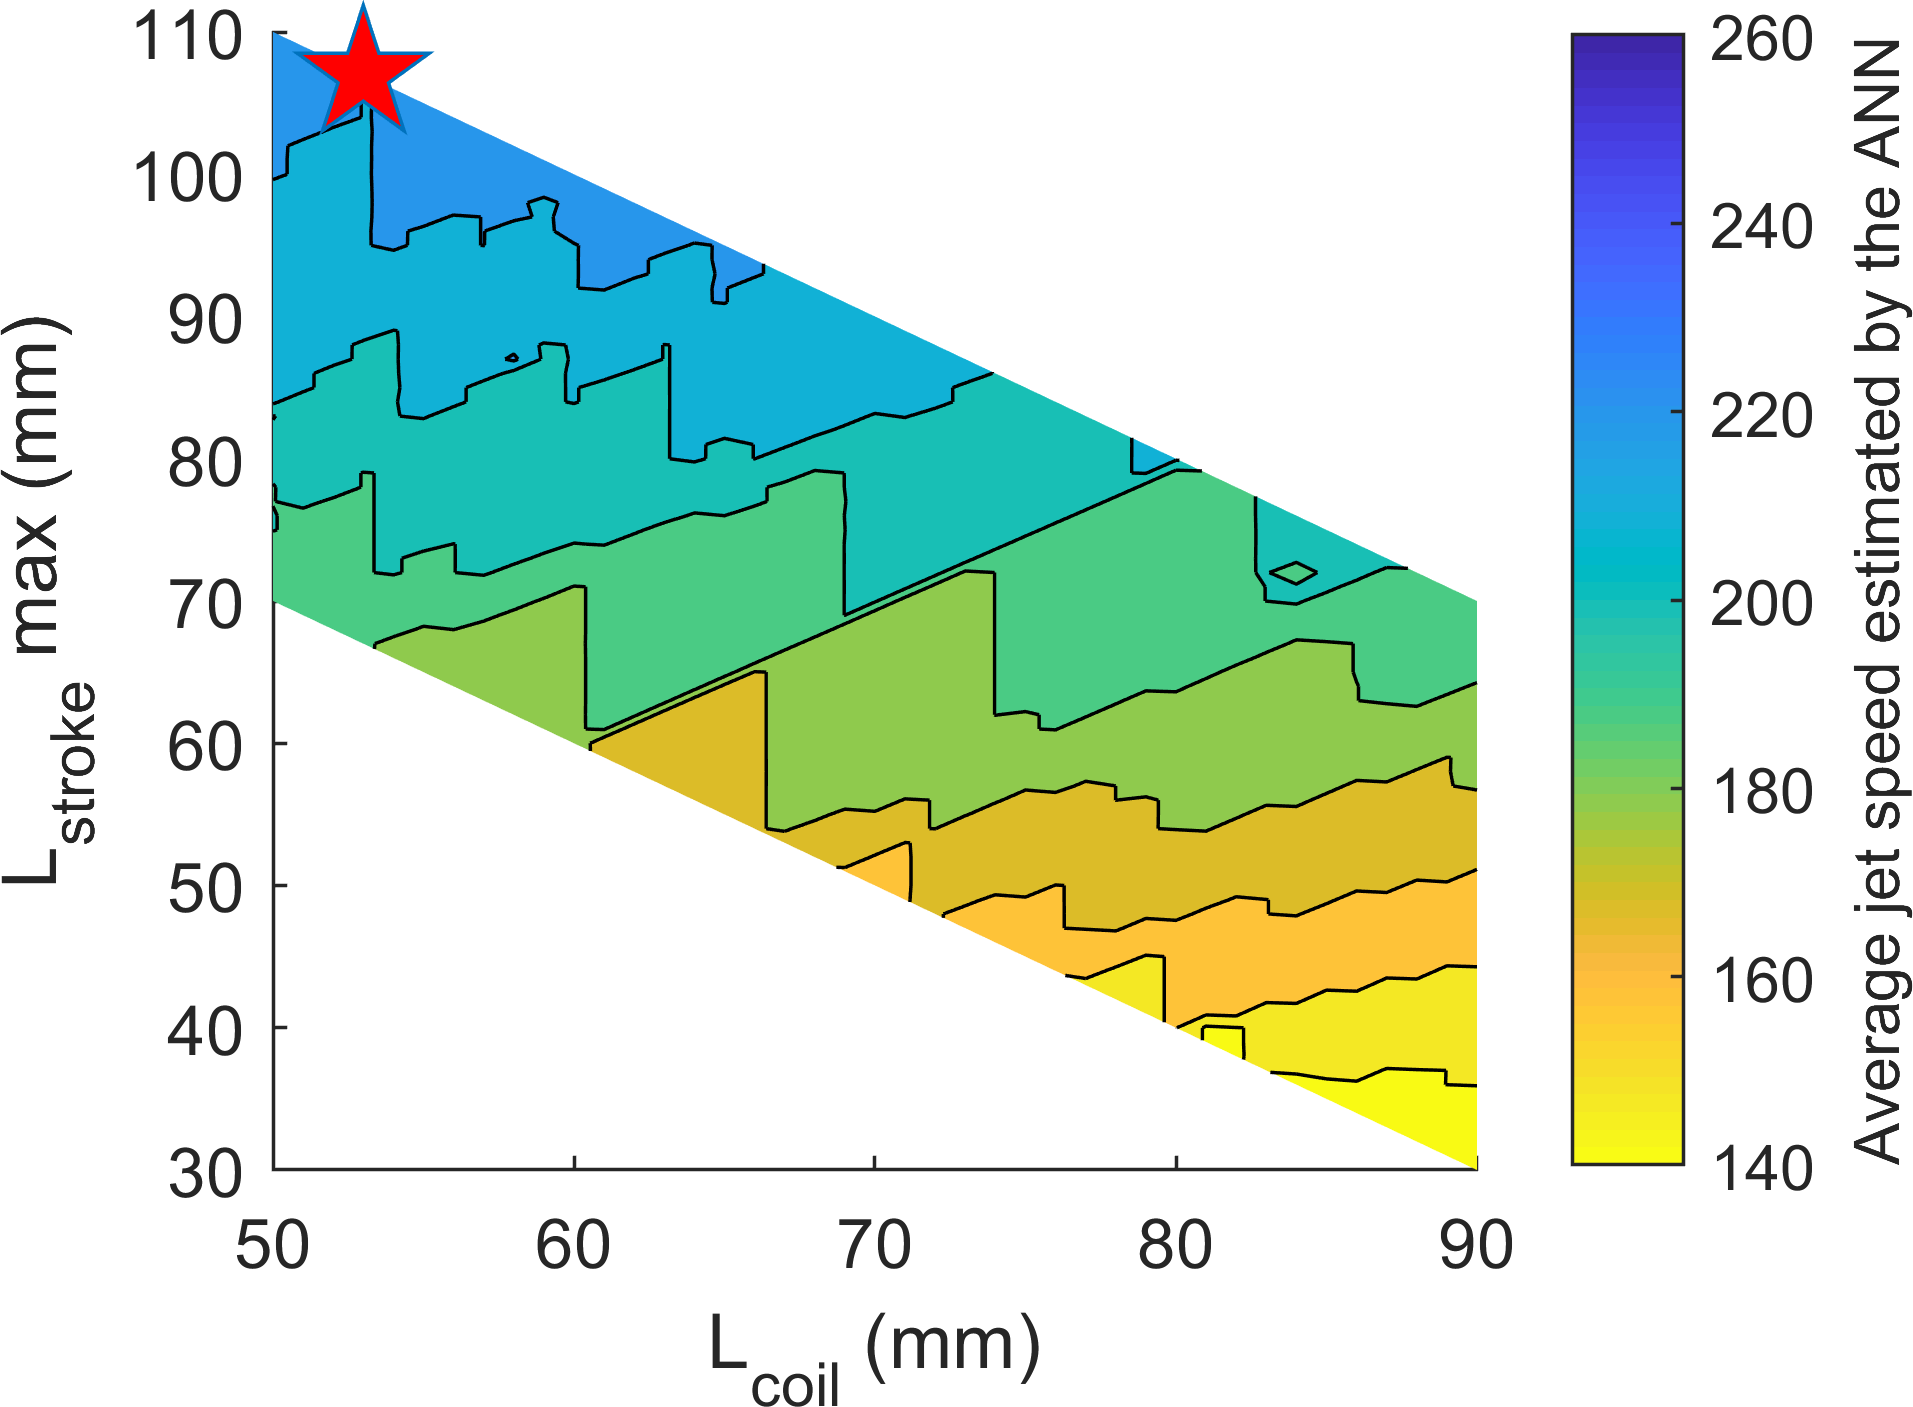
\includegraphics[width=0.45\textwidth]{chap4/images/PMLSM_RSM_325g.png}
                    \label{fig:chapter/rsm/PMLSM/results/325}
                }
                \qquad
                \subfloat[$M_0=350\,\mathrm{g}$ Global optimum found at $L_{C0}=53\,\mathrm{mm}$, $L_{C0}=160\,\mathrm{mm}$, $N_C=3$, and $N_M=9$.
                ]{
                    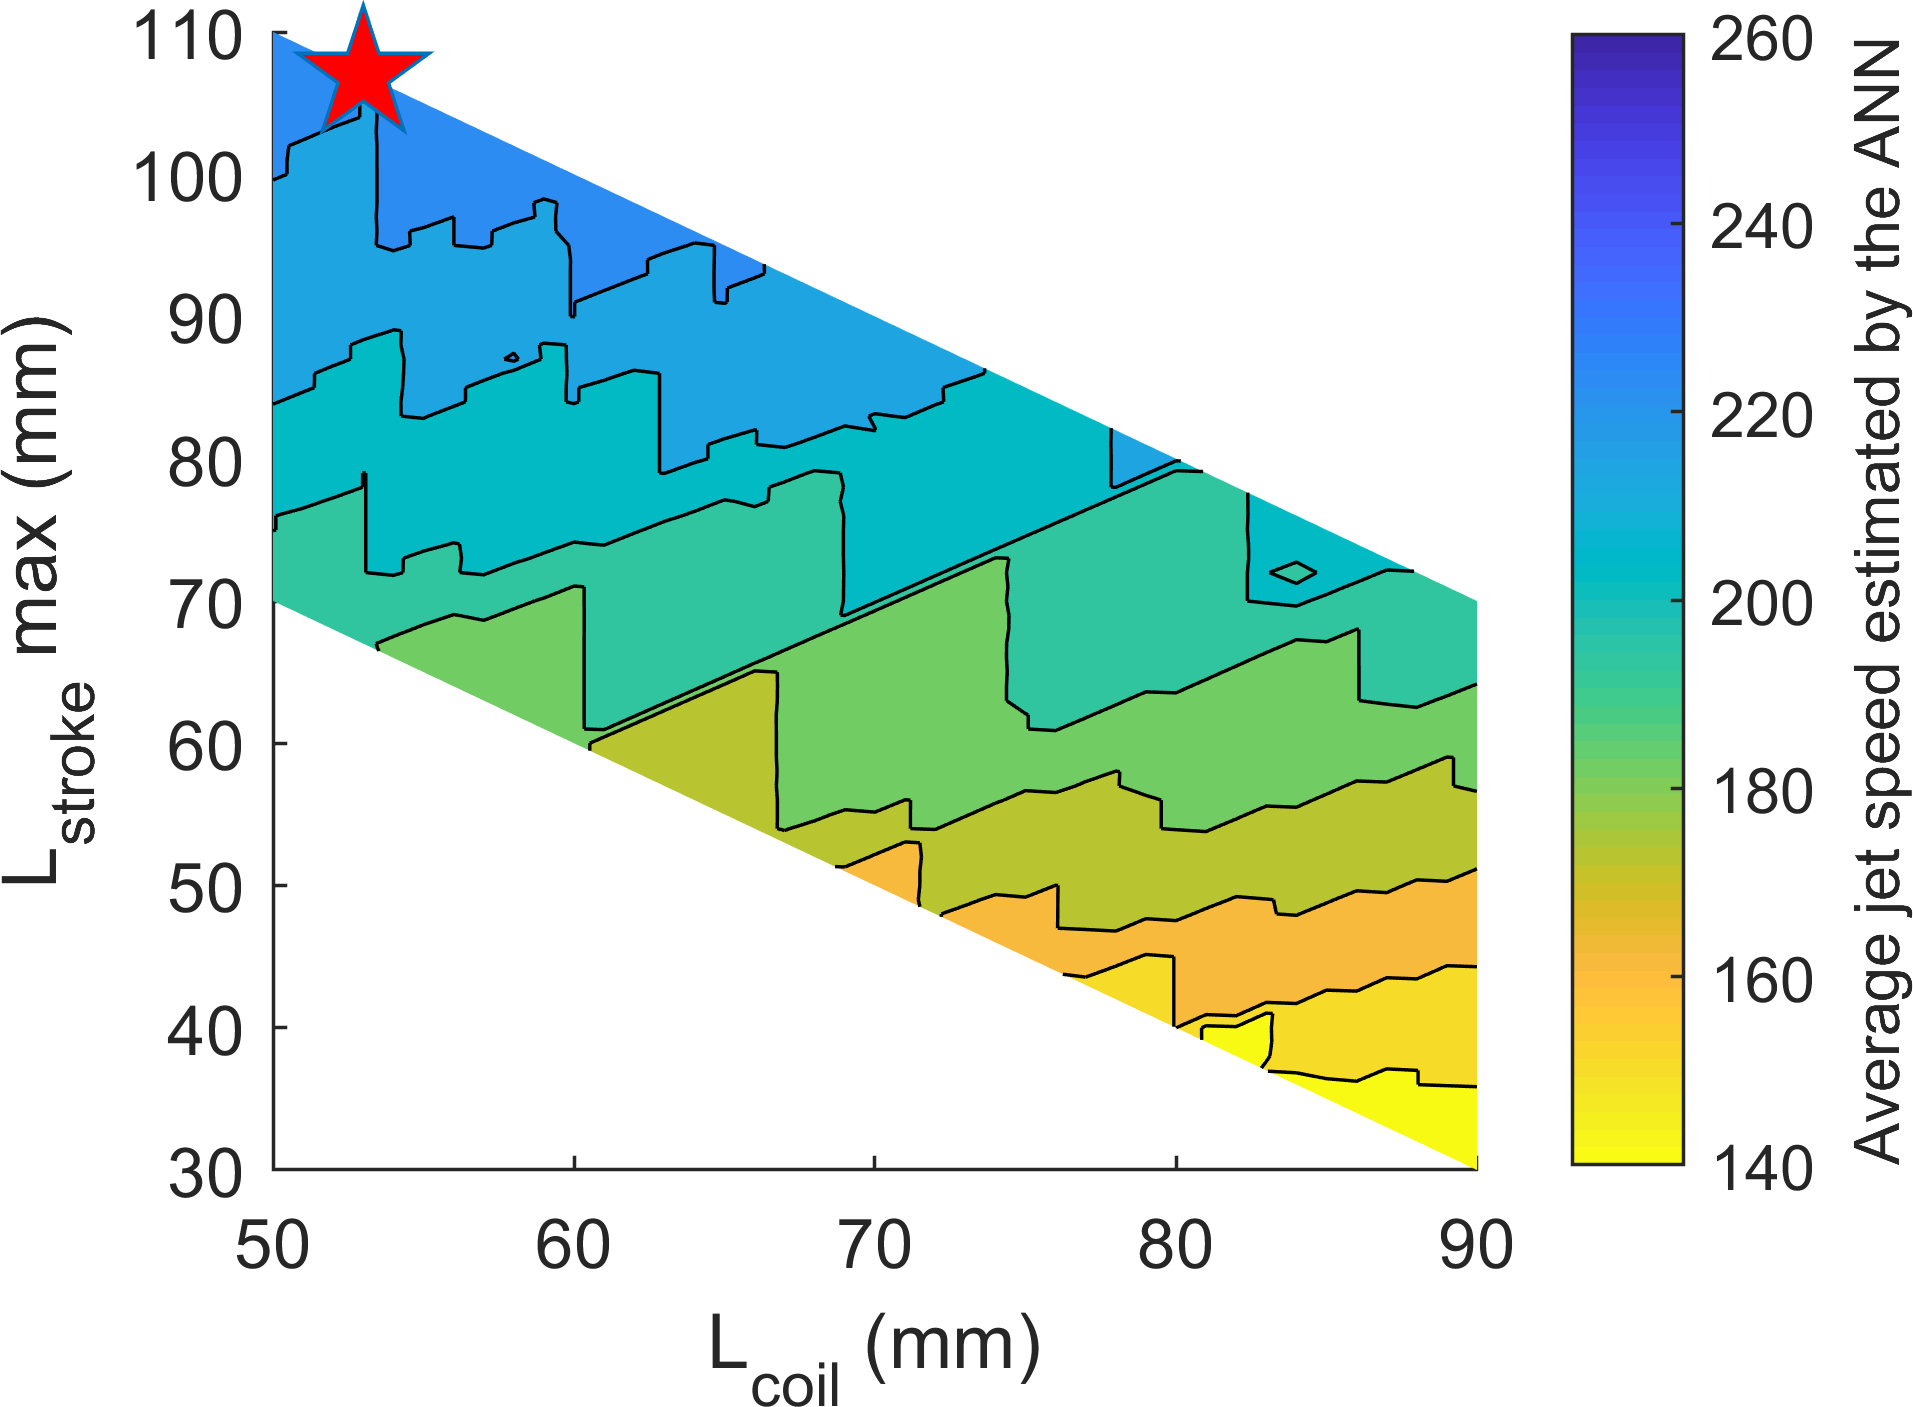
\includegraphics[width=0.45\textwidth]{chap4/images/PMLSM_RSM_350g.png}
                    \label{fig:chapter/rsm/PMLSM/results/350}
                }
                \\
                \subfloat[$M_0=375\,\mathrm{g}$. Global optimum found at $L_{C0}=53\,\mathrm{mm}$, $L_{C0}=160\,\mathrm{mm}$, $N_C=3$, and $N_M=9$.
                ]{
                    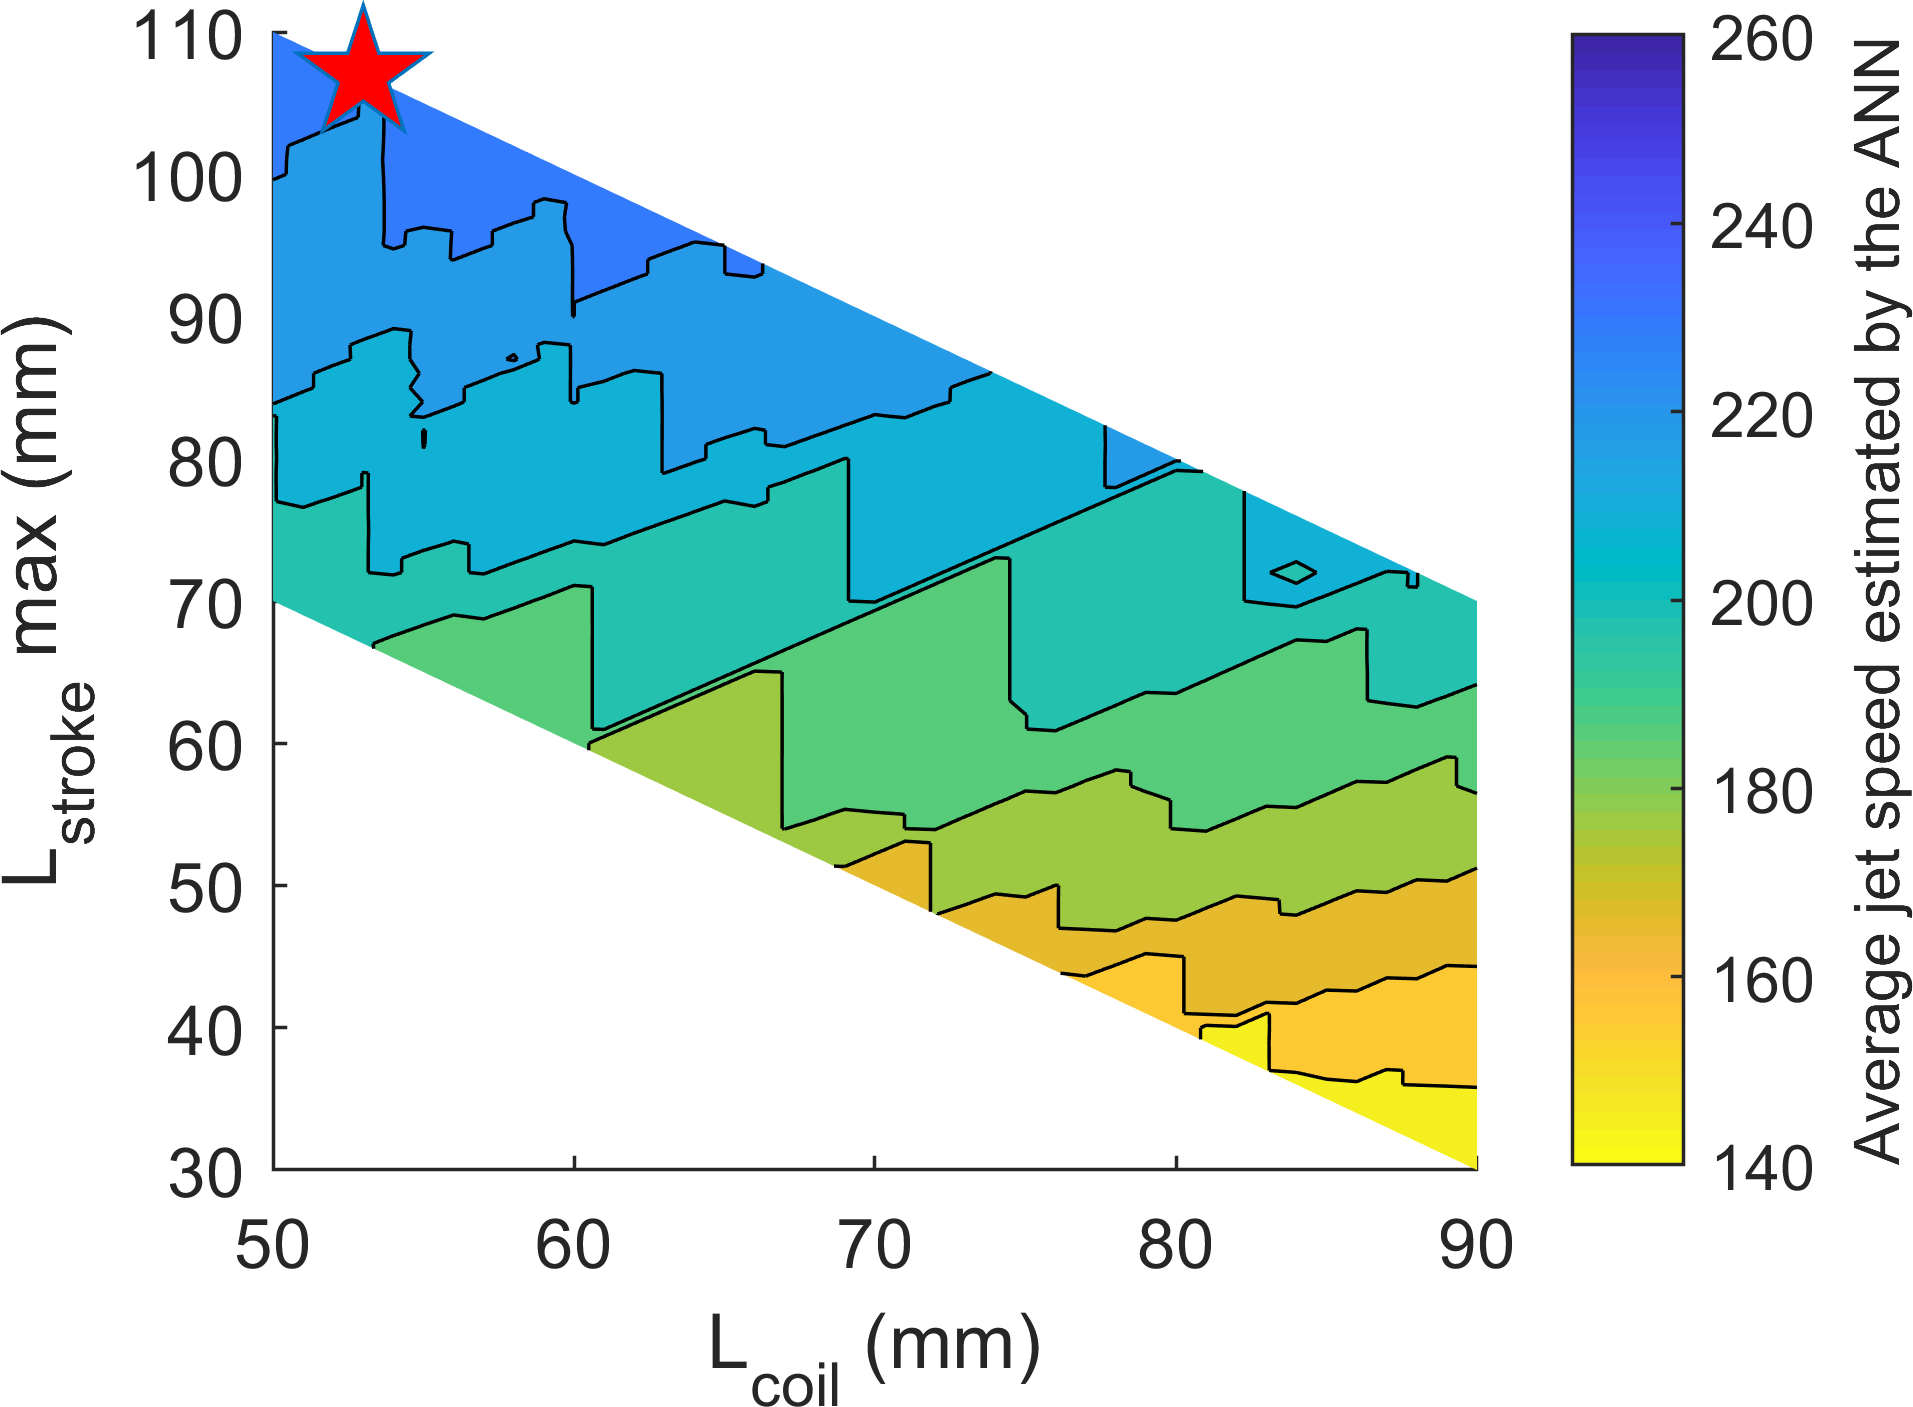
\includegraphics[width=0.45\textwidth]{chap4/images/PMLSM_RSM_375g.png}
                    \label{fig:chapter/rsm/PMLSM/results/375}
                }
                \qquad
                \subfloat[$M_0=400\,\mathrm{g}$. Global optimum found at $L_{C0}=53\,\mathrm{mm}$, $L_{C0}=160\,\mathrm{mm}$, $N_C=3$, and $N_M=9$.
                ]{
                    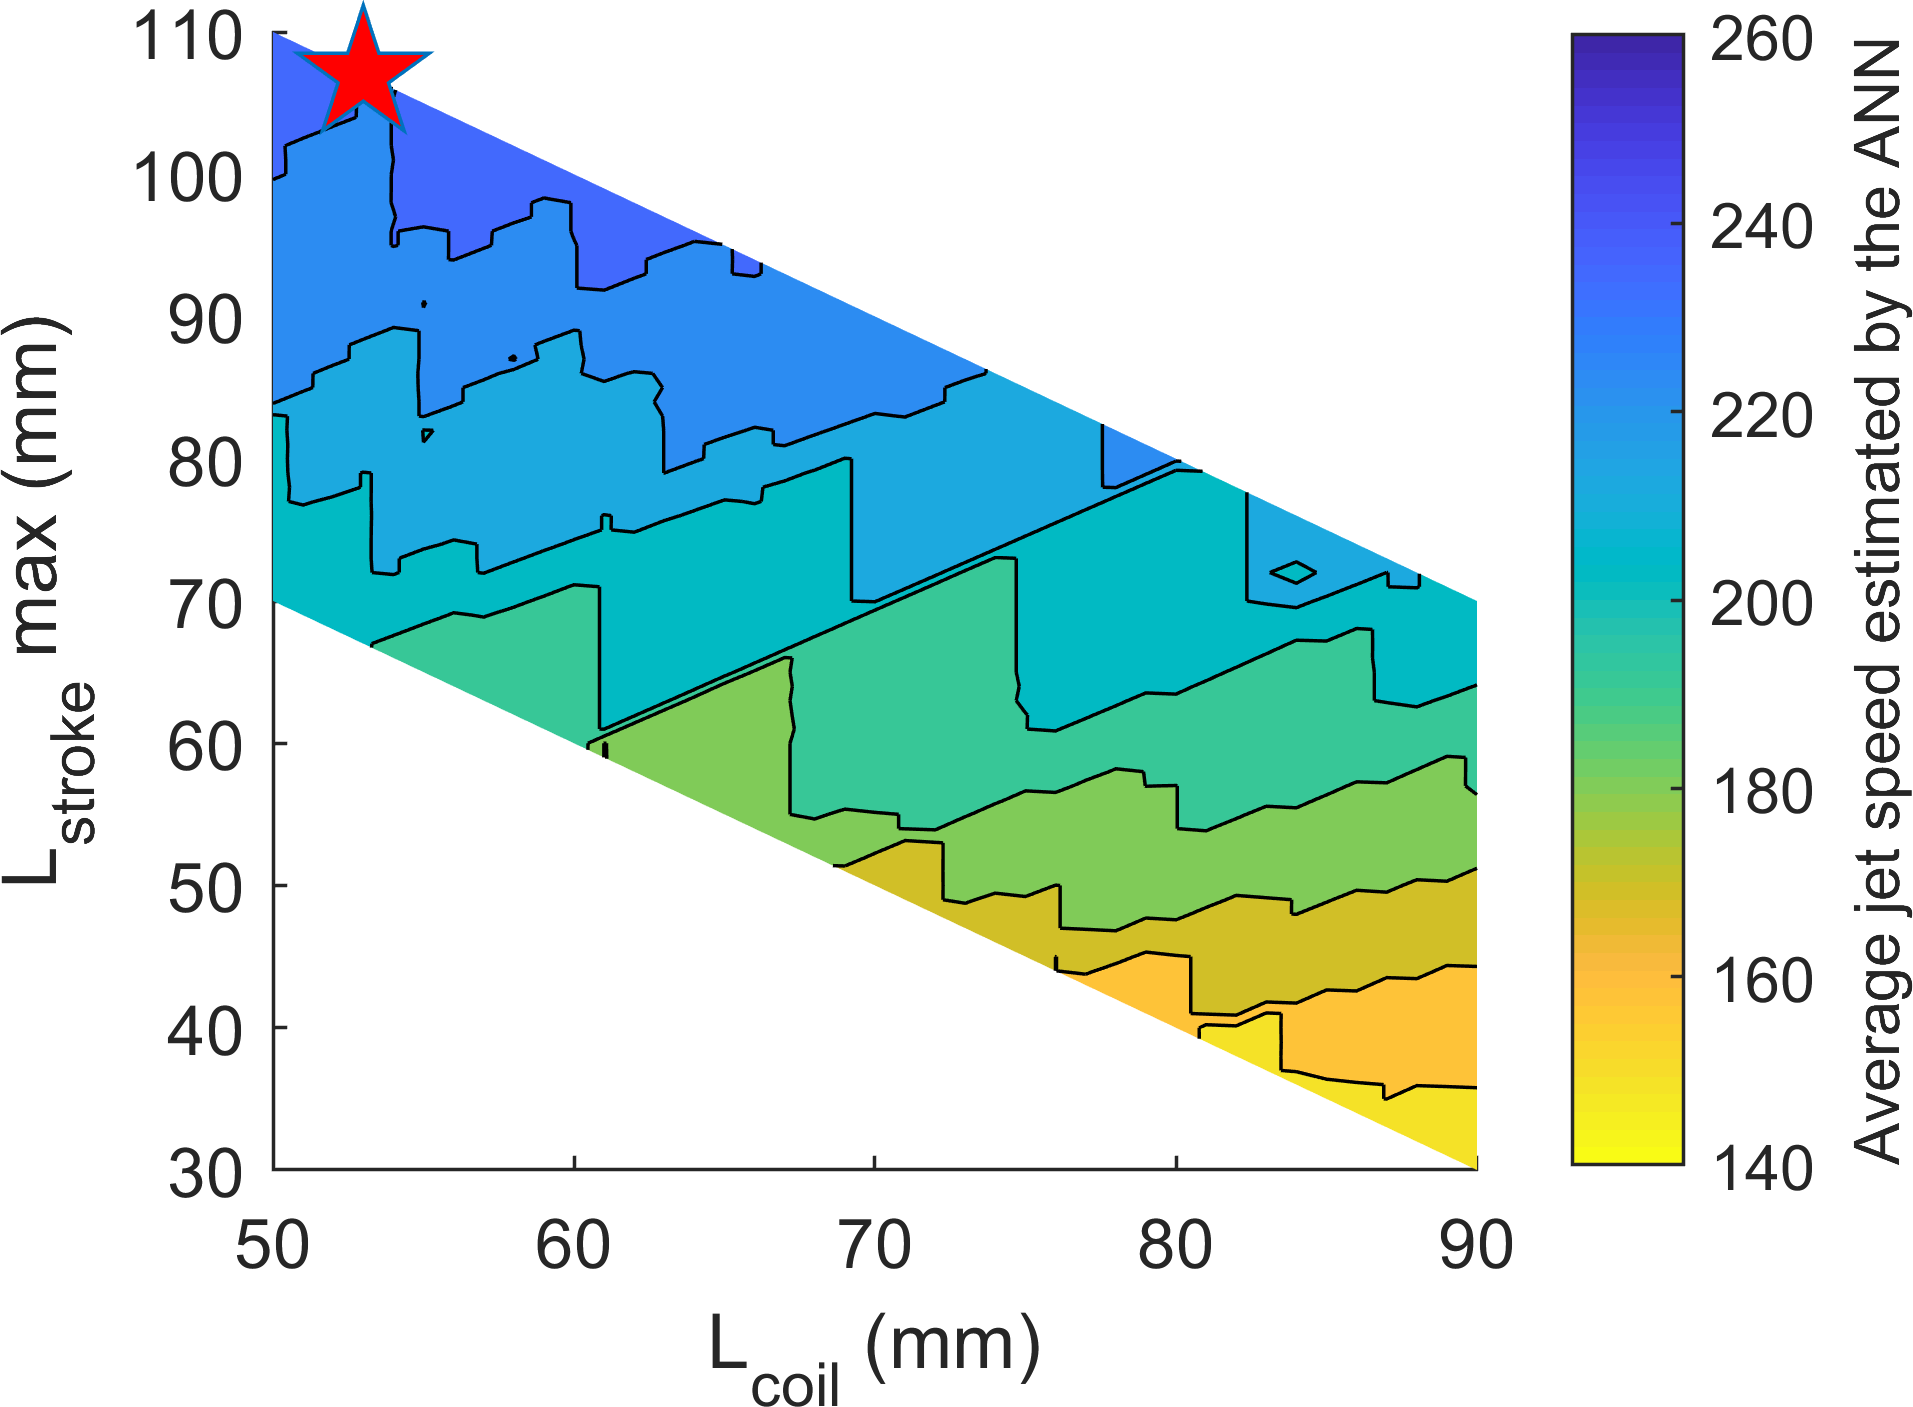
\includegraphics[width=0.45\textwidth]{chap4/images/PMLSM_RSM_400g.png}
                    \label{fig:chapter/rsm/PMLSM/results/400}
                }
                \\
                \subfloat[$M_0=425\,\mathrm{g}$. Global optimum found at $L_{C0}=53\,\mathrm{mm}$, $L_{C0}=160\,\mathrm{mm}$, $N_C=3$, and $N_M=9$.
                ]{
                    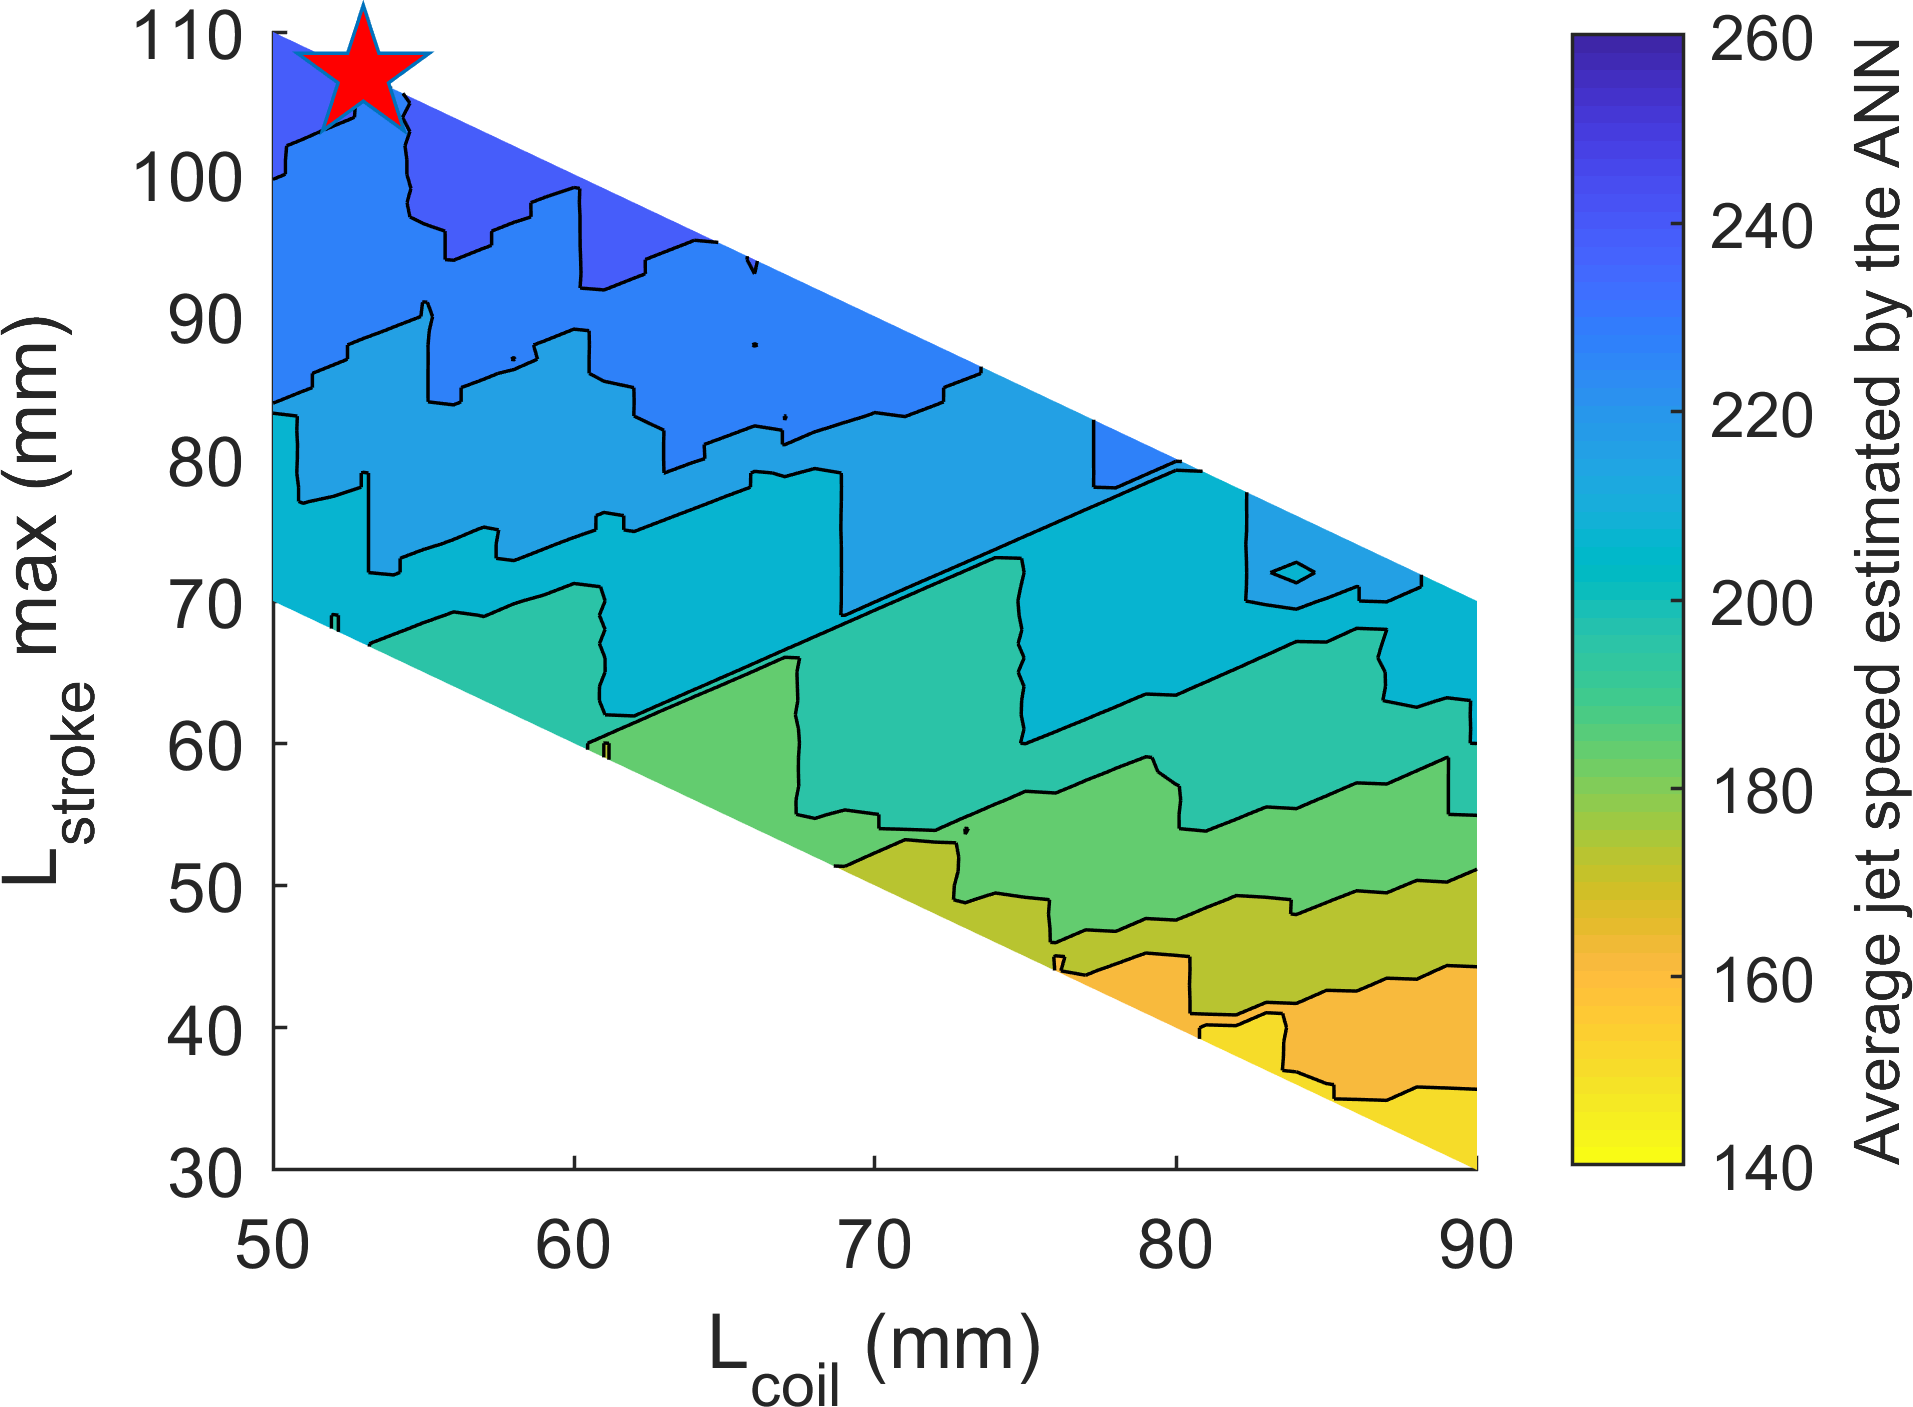
\includegraphics[width=0.45\textwidth]{chap4/images/PMLSM_RSM_425g.png}
                    \label{fig:chapter/rsm/PMLSM/results/425}
                }
                \\
                \caption{
                    The global optimization plots of $v_{jet}$ for the search space $L_{M0}:120\,\mathrm{mm}\rightarrow 160\,\mathrm{mm} \times L_{C0}:50\,\mathrm{mm}\rightarrow 90\,\mathrm{mm}$ using $P=1500\,\mathrm{W}$, $V=1\,\mathrm{mL}$, $gap_{mc}=1.2\,\mathrm{mm}$, $gap_{cf}=0.1\,\mathrm{mm}$,  and $M_0$ of: (a) $325\,\mathrm{g}$, (b) $350\,\mathrm{g}$, (c) $375\,\mathrm{g}$, (d) $400\,\mathrm{g}$, and (e) $425\,\mathrm{g}$.
                }   \label{fig:chapter/rsm/PMLSM/results}
            \end{figure*}
    
    % ===================================================================================================
    % === NEW SECTION === NEW SECTION === NEW SECTION === NEW SECTION === NEW SECTION === NEW SECTION ===
    % ===================================================================================================
    \section{Application to LFSM}               \label{Chapter:RSM/LFSM}
    
    
        This study attempts to clarify the performance characteristics of \acsp{LFSM} when applied to \acs{NFJI} applications. The C-core topology was the most favourable, because they typically produce more thrust than E-core topologies \cite{Min2011}. A conventional 6 slot/5 pole \acs{LFSM} as shown in Fig.\,\ref{fig:chapter/rsm/LFSM/structure/6-5} has minimal thrust ripple due to cancellation of even order and third order harmonics. However, this work chose to study a 6 slot/7 pole LFSM structure as illustrated  in Fig.\,\ref{fig:chapter/rsm/LFSM/structure/6-7} because it is reported to also produce more thrust than other configurations, even though it may come at the expense of having more thrust ripple \cite{Chen2010}. 
        
        
        \begin{figure*}[!ht]
            \centering
            \subfloat[\label{fig:chapter/rsm/LFSM/structure/6-7}Tubular LFSM with 6 slots and 7 poles per period.]{
                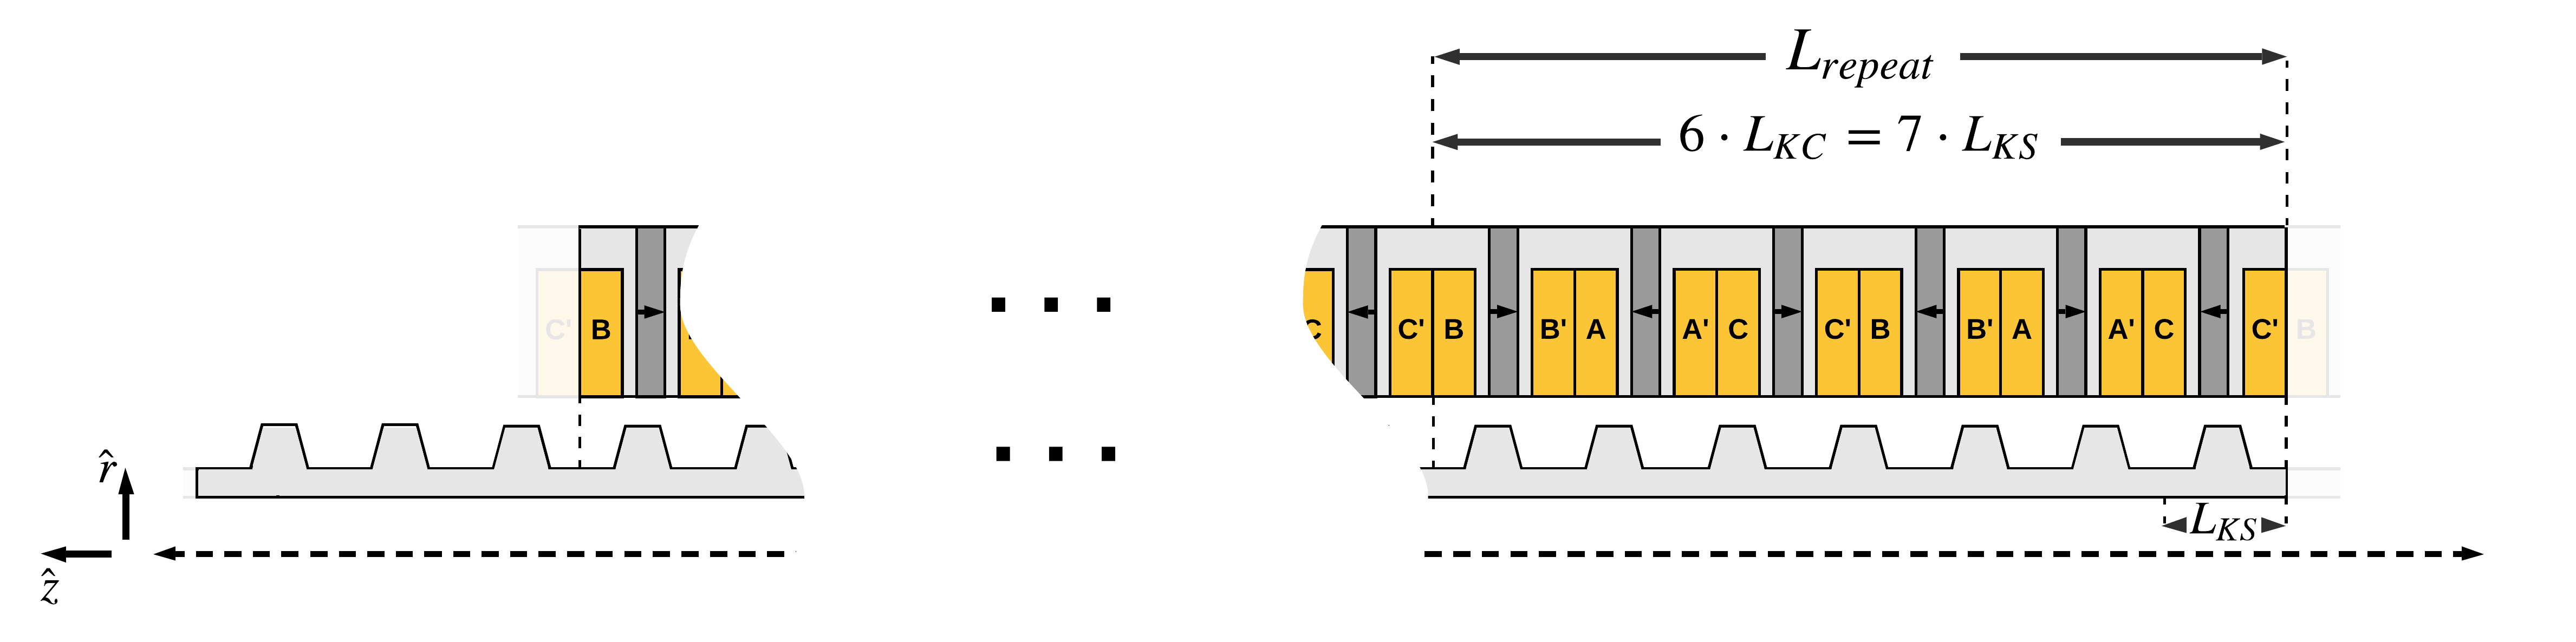
\includegraphics[width=0.97\textwidth]{chap4/images2/LFSM_6_7.png}
            }
            \\
            \subfloat[\label{fig:chapter/rsm/LFSM/structure/6-5}Tubular LFSM with 6 slots and 5 poles per period.]{
                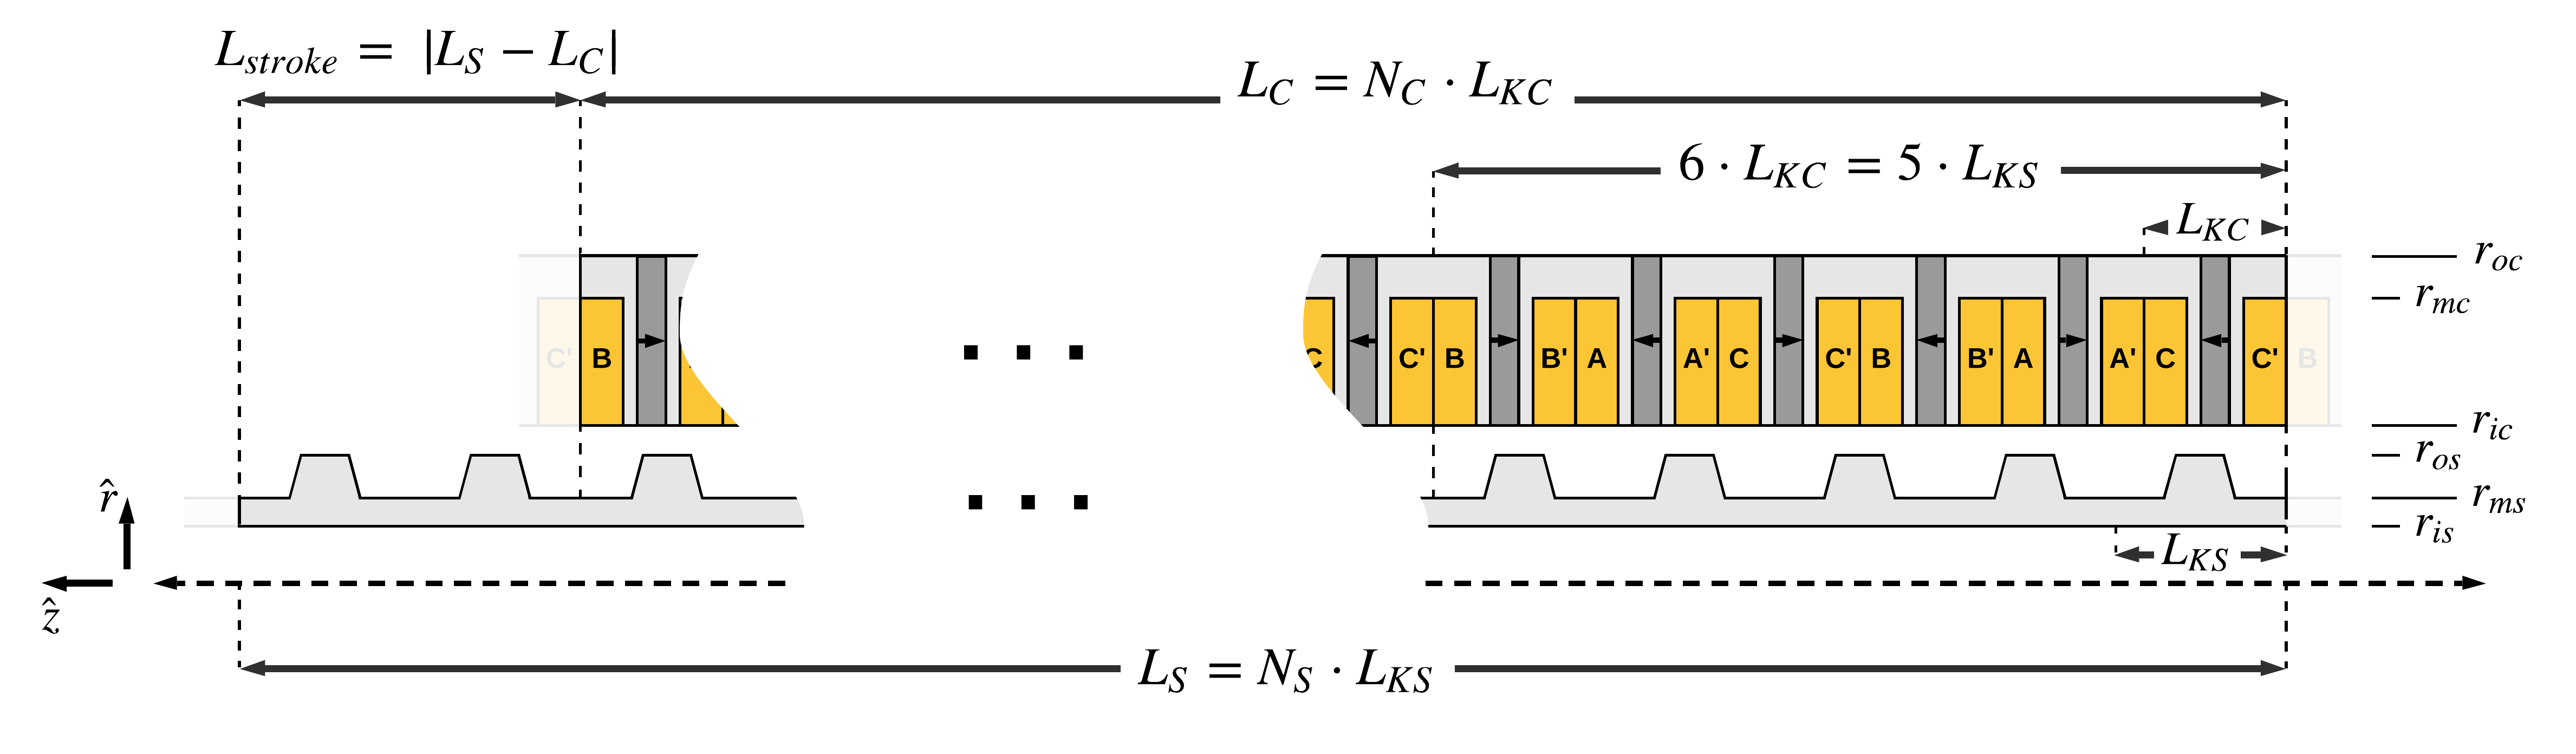
\includegraphics[width=0.97\textwidth]{chap4/images2/LFSM_6_5.png}
            }
            \caption{Schematic of tubular \acs{LFSM}
                \label{fig:conventional_flux_switching_machines}
            }\label{fig:chapter/rsm/LFSM/structure}
        \end{figure*}
        
        
        The general parameters of a three-phase tubular linear flux-switching motor consist of:
        
        \begin{itemize}
            \item The total number of armature slots $N_C$, as opposed to the number of half-coil phases $N_M$ in \acsp{PMLSM},
            \item The total number of armature pole $N_S$, which is different from the number of half-magnet phases in \acsp{PMLSM},
            \item The radii of the \acs{SMC} track $r_{is}$, $r_{ms}$, and $r_{os}$,
            \item The radii of the armature assembly $r_{ic}$, $r_{mc}$, and $r_{oc}$,
            \item The slot period length $L_{KC}$,
            \item The track period length $L_{KS}$,
            \item The whole of mover armature length $L_{C}$,
            \item The whole track length or equivalent motor length $L_{S}$, which does not represent the stroke length like in \acsp{PMLSM},
            \item The length of each overall repeat unit $L_{repeat}$ of $6$ coil slots and $7$ track poles,
            \item The motor stroke length $L_{stroke}$.
        \end{itemize}
        
        
        \begin{figure*}
            \centering
            \subfloat[\label{fig:chapter/rsm/LFSM/machine design/params} Detailed dimensions]{
                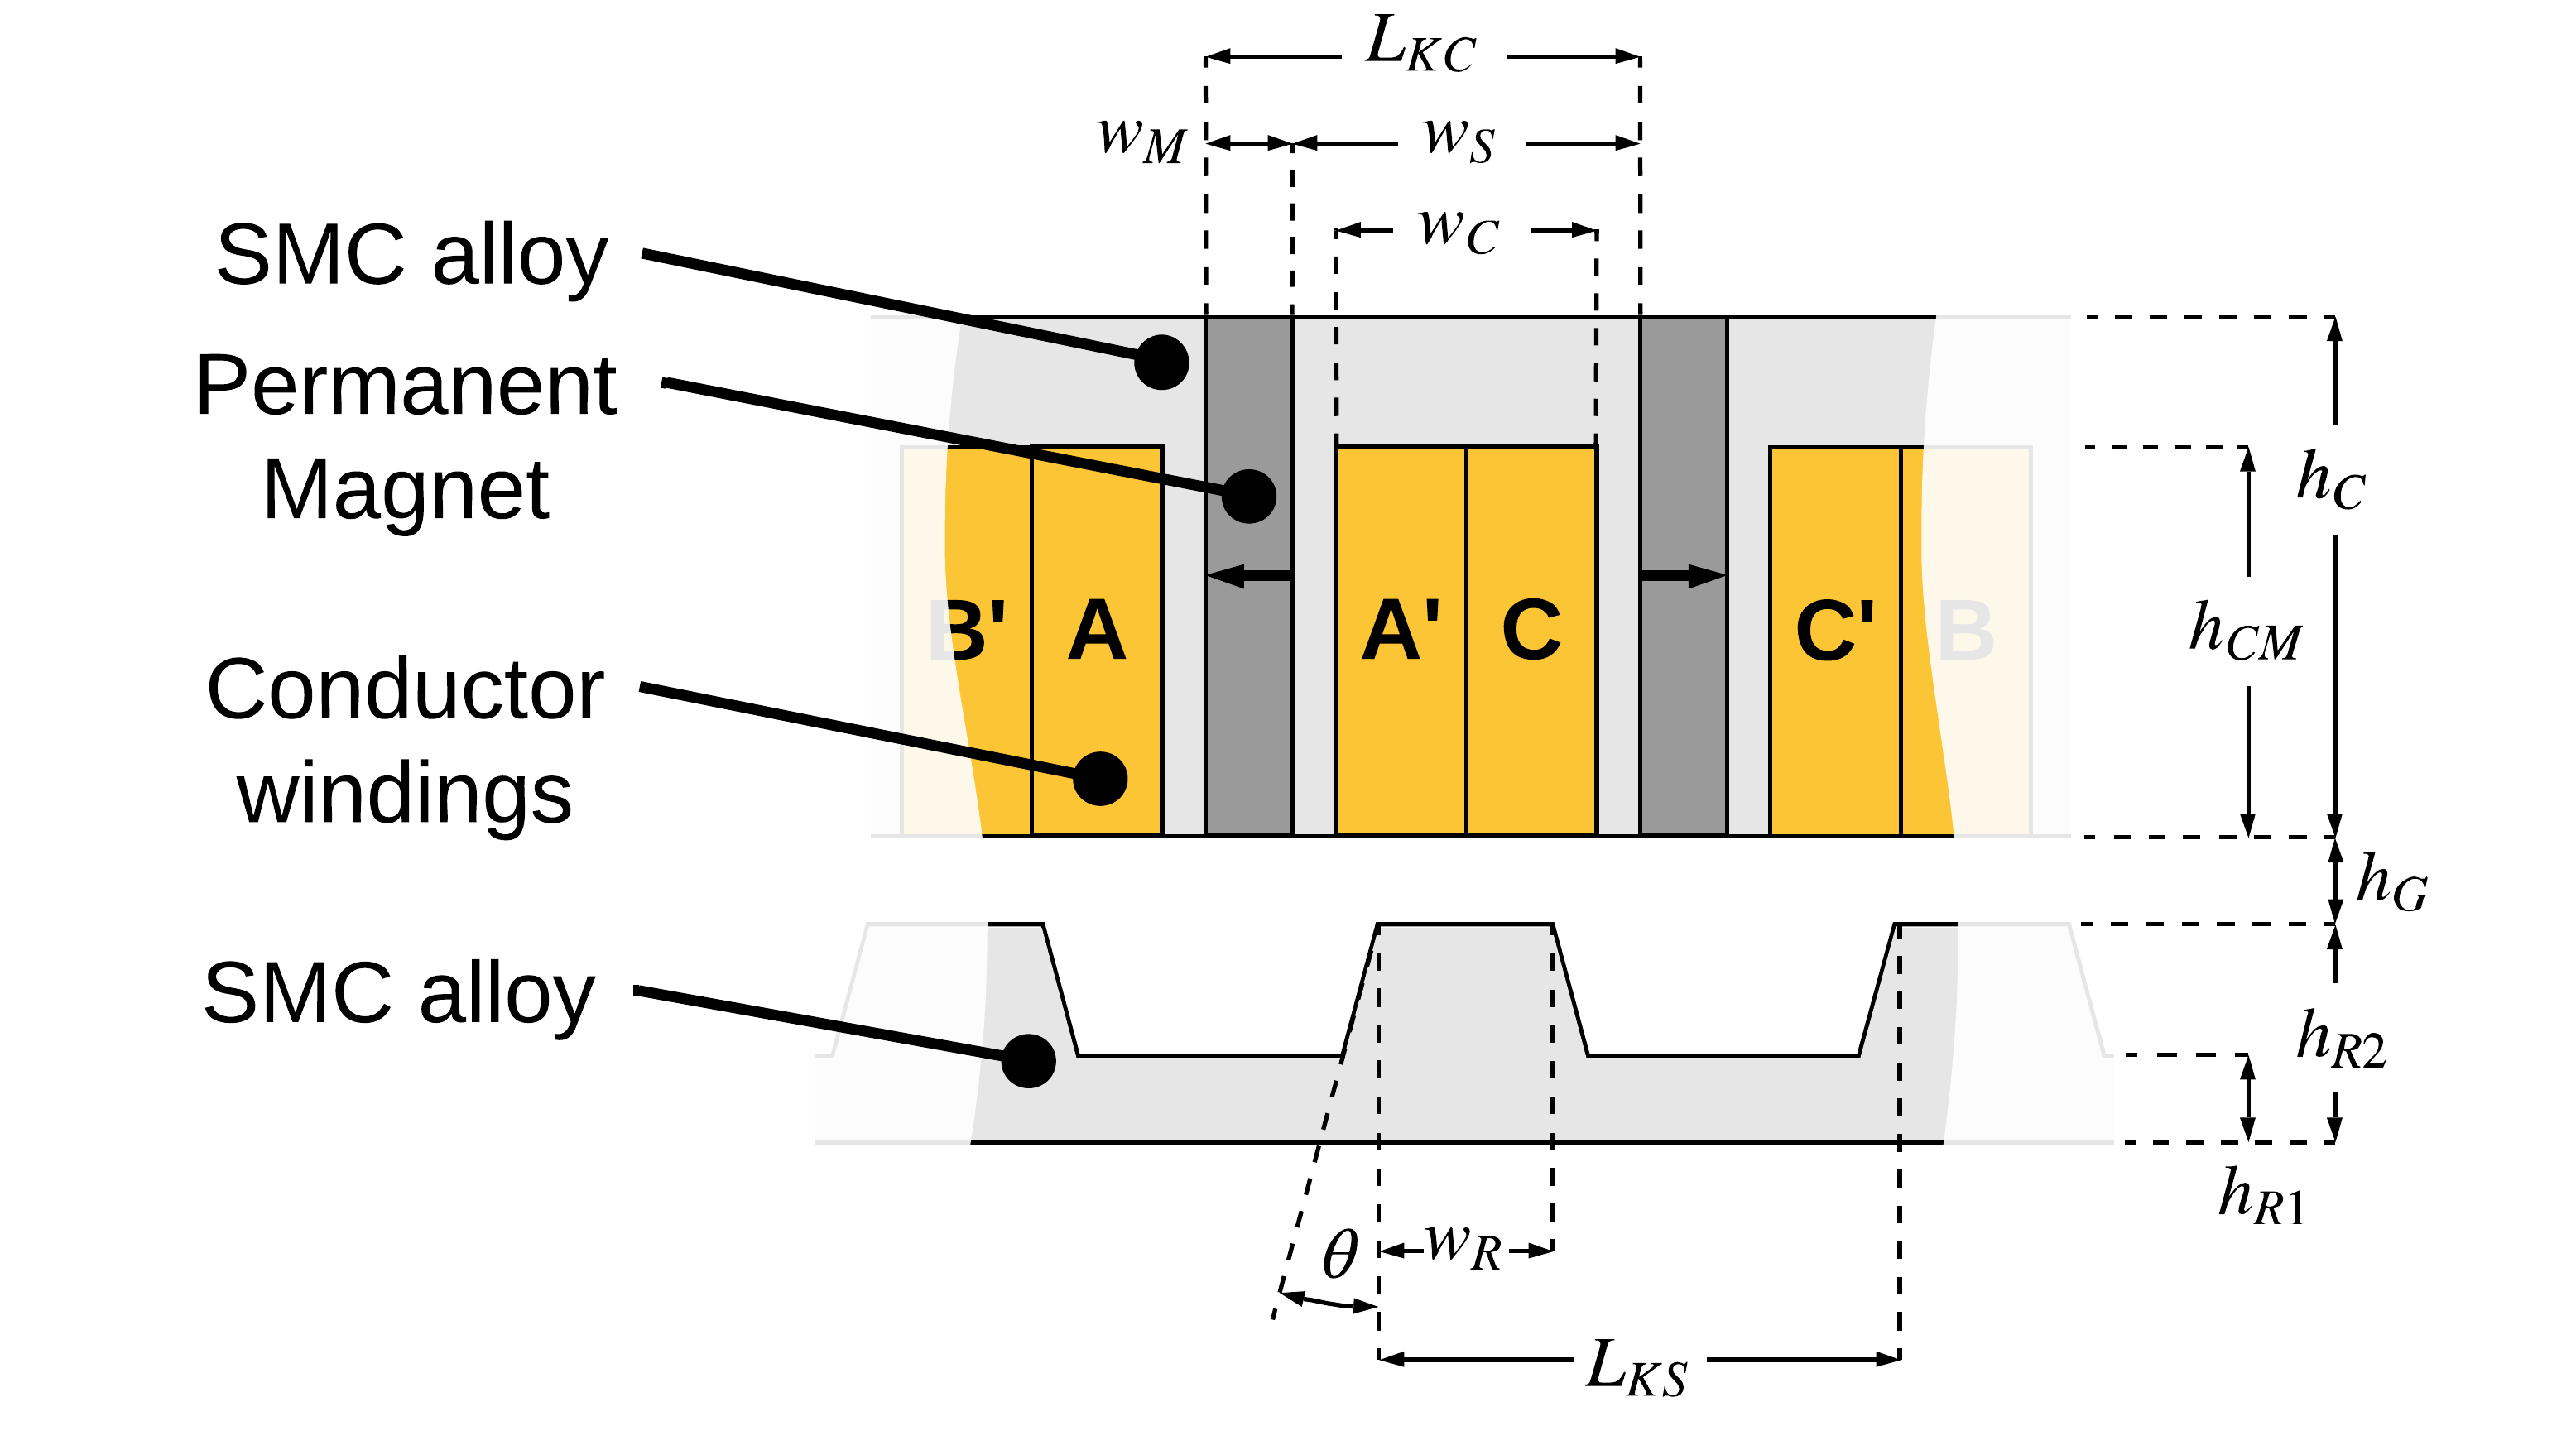
\includegraphics[width=0.7\textwidth]{chap4/images2/params.png}
            }
            \\
            \subfloat[\label{fig:chapter/rsm/LFSM/machine design/setup} A jet injector driven by a LFSM]{
                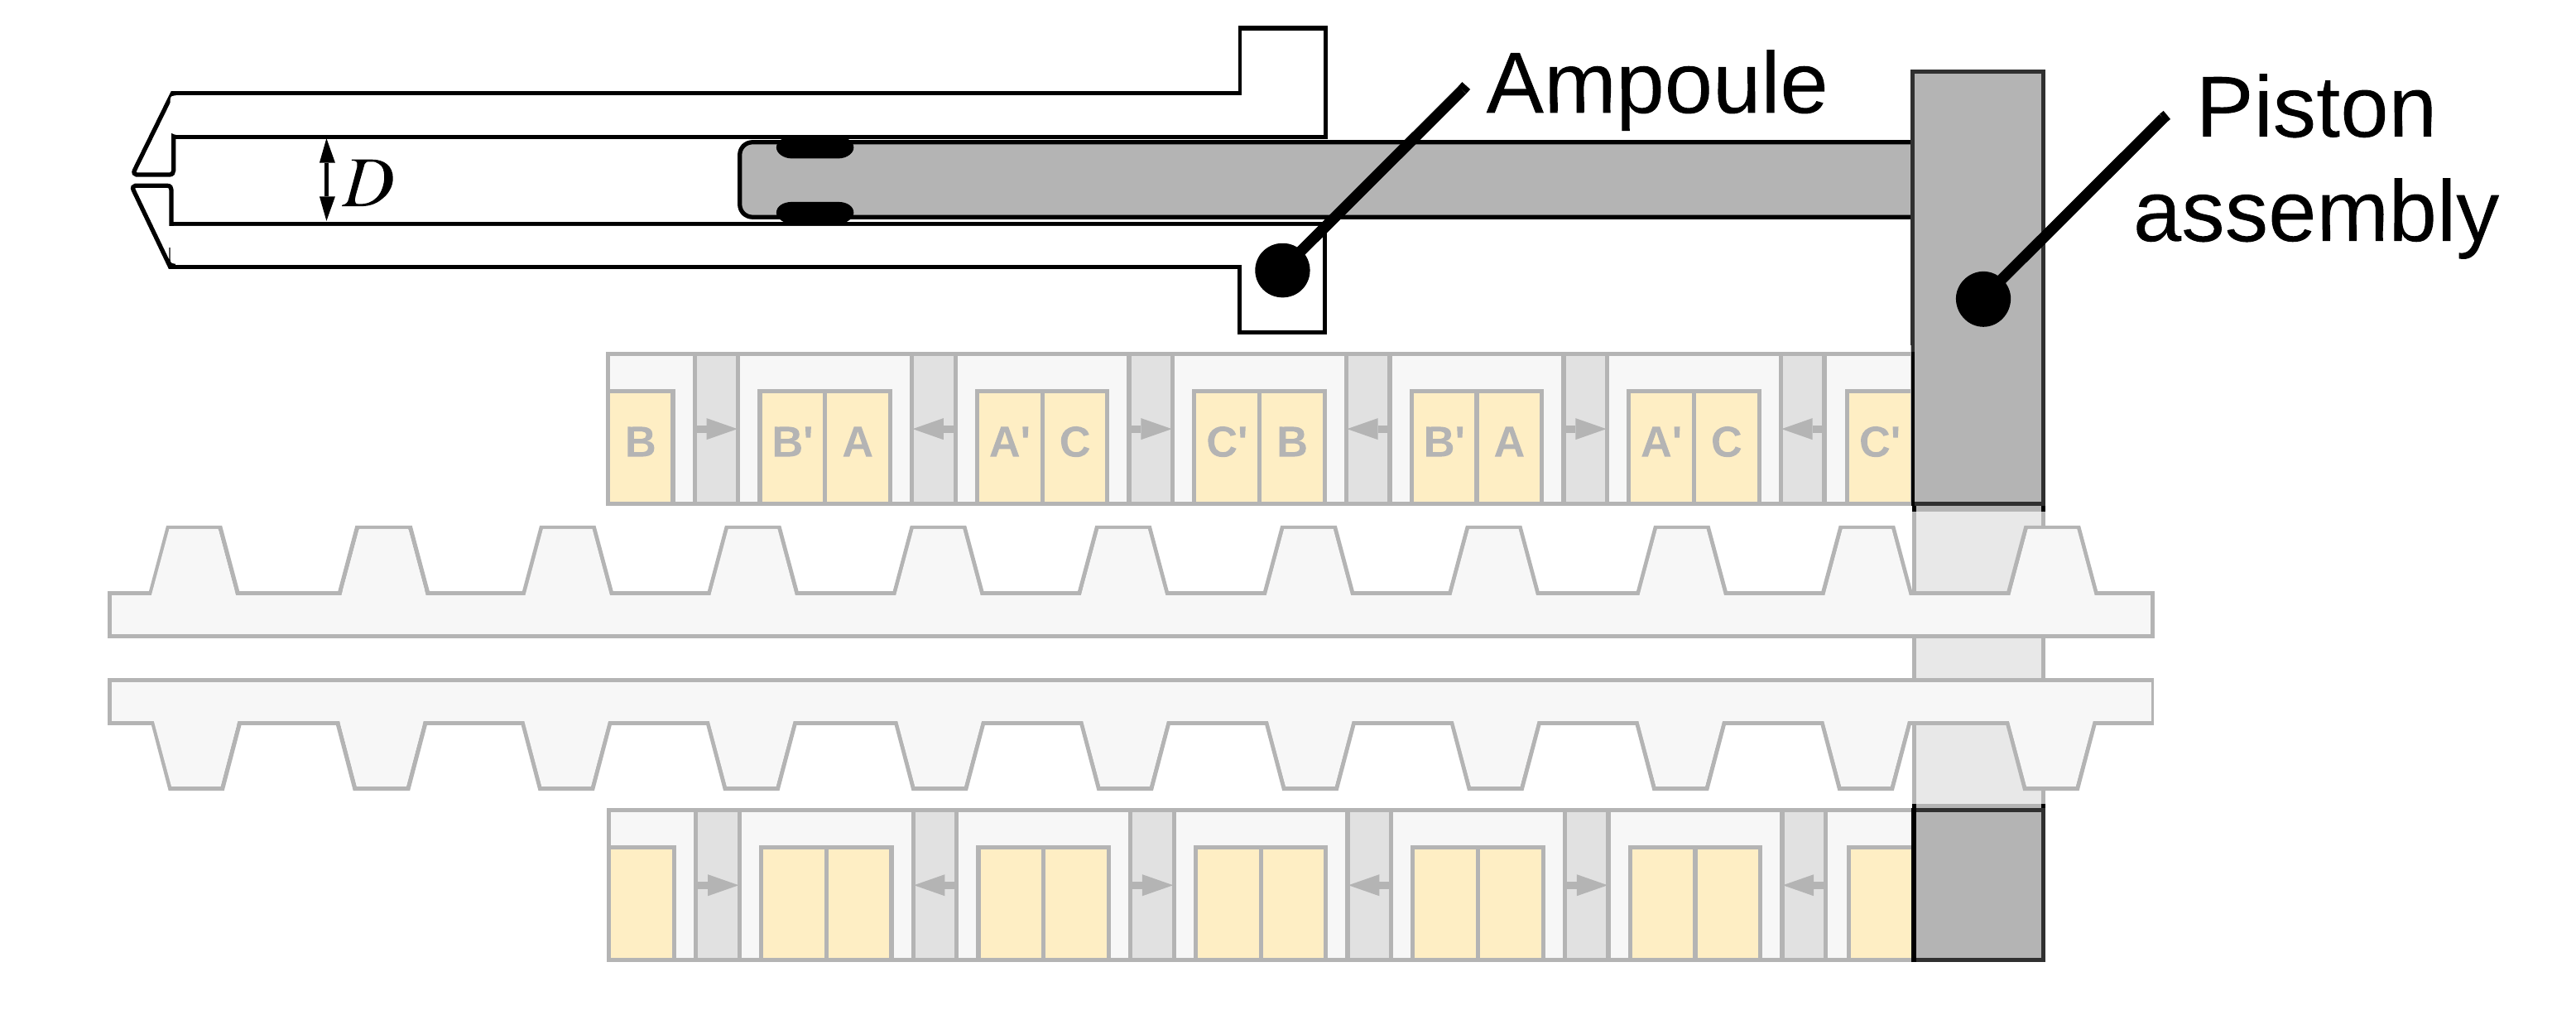
\includegraphics[width=0.8\textwidth]{chap4/images2/machine_setup.png}
            }
            \caption{ 
                \label{fig:chapter/rsm/LFSM/machine design}Detailed dimensions of the tubular LFSM: 
                armature assembly widths ($w_M$, $w_S$, $w_C$),
                armature assembly heights ($h_{CM}$, $h_{C}$),
                track tooth width ($w_{R}$),
                and track tooth heights ($h_{R1}$, $h_{R2}$), tooth angle $\theta$, air gap $h_G$ in $\mathrm{(a)}$. A basic schematic of a LFSM driven jet injector and a NFJI drug ampoule with diameter $D$ are shown in $\mathrm{(b)}$.
            }
        \end{figure*}
        
        
        To minimize the moving (and total) mass, the outer sliding armature assembly was selected as the moving element. Each repeating period of the mover consists of six axially magnetized permanent magnet rings, six \acf{SMC} cylindrical cores to contain the conductor windings, and two circumstantially wound three-phase coil groups. The secondary is passive, and constructed as an SMC tube with a periodic tooth structure with angled sides. Dimensions are shown for each topology in Fig.\,\ref{fig:chapter/rsm/LFSM/machine design/params}. Additionally, Fig.\,\ref{fig:chapter/rsm/LFSM/machine design/setup} illustrates how a tubular \acs{LFSM} can be incorporated in the design of a hand-held jet injector device. Different lengths of the topology are governed by the following equations:
        
        
        \begin{equation}
            L_{repeat}=6\,L_{KC}=7\,L_{KS}
            \label{eq:chap/rsm/LFSM/L_repeat,LKC,LKS}
        \end{equation}
        
        \begin{equation}
            L_{C}=N_C\,L_{KC}
            \label{eq:chap/rsm/LFSM/L_C}
        \end{equation}
        
        \begin{equation}
            L_{S}=N_S\,L_{KS}
            \label{eq:chap/rsm/LFSM/L_S}
        \end{equation}
        
        
        \begin{equation}
            L_{stroke}= \big| L_S-L_C \big|
            \label{eq:chap/rsm/LFSM/L_stroke}
        \end{equation}
        
        
        Additional design ratios were established to better capture the parametric representation of the 6 slot/7 pole tubular \acs{LFSM}:
        
        
        \begin{equation}
            \alpha=\frac{w_M}{L_{KC}}
            \label{eq:chap/rsm/LFSM/alpha}
        \end{equation}
        
        
        \begin{equation}
            \beta=\frac{w_C}{w_S}
            \label{eq:chap/rsm/LFSM/beta}
        \end{equation}
        
        
        \begin{equation}
            \gamma=\frac{h_{CM}}{h_C}
            \label{eq:chap/rsm/LFSM/gamma}
        \end{equation}
        
        
        \begin{equation}
            \delta=\frac{w_R}{L_{KS}}
            \label{eq:chap/rsm/LFSM/delta}
        \end{equation}
        
        
        \begin{equation}
            \epsilon=\frac{h_{R1}}{h_{R2}}
            \label{eq:chap/rsm/LFSM/epsilon}
        \end{equation}

    
        In later subsections, the aim of the work is to examine the performance of \acs{LFSM} for \acs{NFJI} tasks using a process described in Section\,\ref{Chapter:RSM/outline} and demonstrated in Section\,\ref{Chapter:RSM/PMLSM}. Fig.\,\ref{fig:chapter/rsm/LFSM/design process} illustrates the \acs{RSM} design process adapted to the \acs{LFSM} topology above. 
    
    
        \begin{figure*}
            \centering
            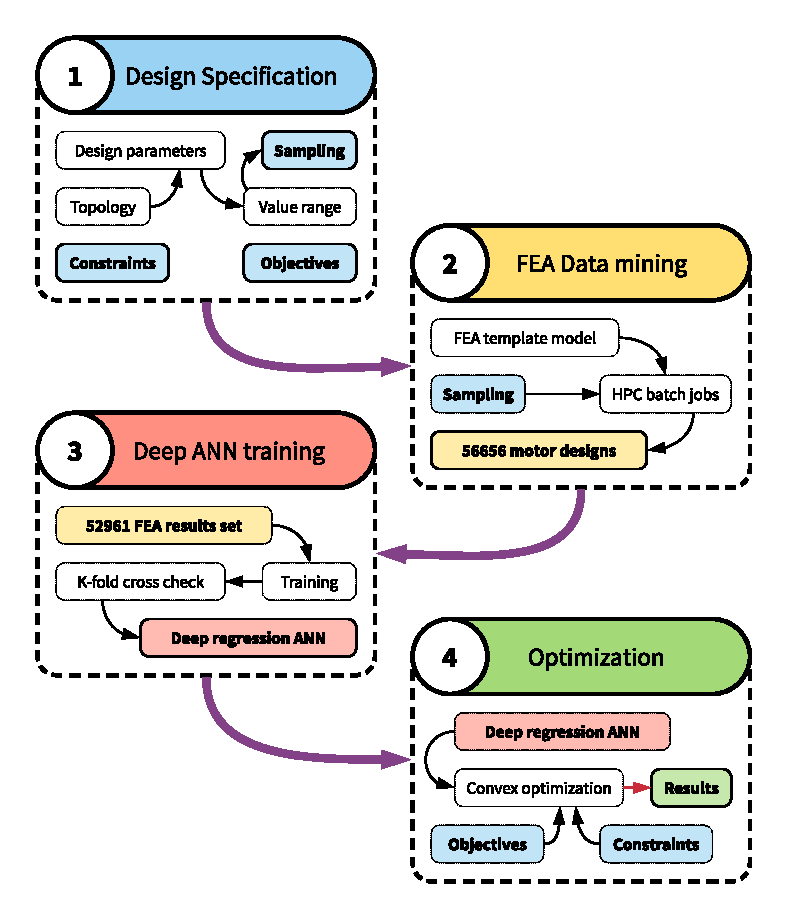
\includegraphics[width=4.5in]{chap4/images2/LFSM_design_process.pdf}
            \caption{Flowchart of the RSM motor design process adapted for \acs{LFSM}.}
            \label{fig:chapter/rsm/LFSM/design process}
        \end{figure*}
    
    
        % -----------------------------------------------------------------------------------
        % --- NEW SUB SECTION --- NEW SUB SECTION --- NEW SUB SECTION --- NEW SUB SECTION --- 
        % -----------------------------------------------------------------------------------
        \subsection{Specifications \& Samplings}    \label{Chapter:RSM/LFSM/spec}
        
        
            This work investigated and optimized a tubular linear 6 slot/7 pole machine with the dimensions presented in Fig.\,\ref{fig:chapter/rsm/LFSM/structure} and \,\ref{fig:chapter/rsm/LFSM/machine design}. With consideration to the dimensions and ratios of the desired motor design, the structural design factors and their range are summarized in Table\,\ref{table:chap/rsm/LFSM/design range}. 
            
            
            The magnet, conductor and \acs{SMC} core assembly as a whole body was treated as the mover, and the \acs{SMC} track with trapezoid teeth was treated as the stator. Similar to the tubular \acs{PMLSM}, the stator core inner radius $r_{si}$ and the mover-stator air gap $h_G$ are fixed at $2\mathrm{mm}$ and $1.2\mathrm{mm}$, respectively. With an effective stator pocket of $4\,\mathrm{mm}$ in diameter, the structural support has a space to be added later on. For the ease of manufacturing, there required a reasonable amount of air gap between the stator and mover such as $1.2\mathrm{mm}$, which comes from our past experience building tubular longitudinal synchronous motor. Physically, this air gap will include non-magnetic support structures as well as mechanical clearance. Note that in the data collection process, the motor length $L_S$ and stroke length $L_{stroke}$ were yet to be determined. Instead, the length of each repeat 6 slot/7 pole unit $L_{repeat}$ was iterated upon. To simplify the model, the tooth angle $\theta$ was set to be a fixed value of $\arctan{1/2}$, which makes the width of each tooth extension precisely half the height of the teeth.
            
            
            Table\,\ref{table:chap/rsm/LFSM/sampling levels} shows incremental sampling steps for the structural design factors. From the sampling steps, a design grid of $46656$ cases was generated. Additionally, another $10000$ cases constructed by input variables created with random values within Table\,\ref{table:chap/rsm/LFSM/design range} range were added to help generalize the entire continuous design space better. In total, there were $56656$ independent motor designs to have their average thrust, maximum thrust, and cogging profile predicted by \acs{FEA}.
            
            
            \begin{table}
                \renewcommand{\arraystretch}{1.2}
                \caption{Summary of the \acs{LFSM} motor parameter ranges}
                \label{table:chap/rsm/LFSM/design range}
                \centering
                \begin{tabular}{@{}llr@{}}
                \hline
                \bfseries Parameter & \bfseries Description & \bfseries Values\\
                \hline
                    $\alpha$	    & Ratio of $w_M$ over $L_{KC}$              &	$0.1-0.4$\\ 
                    $\beta$	        & Ratio of $w_C$ over $w_S$		            &	$0.4-0.9$\\ 
                    $\gamma$	    & Ratio of $h_{CM}$ over $h_C$			    &	$0.6-0.9$\\ 
                    $\delta$	    & Ratio of $w_R$ or $L_{KS}$		        &	$0.1-0.3$\\ 
                    $\epsilon$	    & Ratio of $h_{R1}$ or $h_{R2}$		        &	$0.4-0.6$\\ 
                    $r_{si}$	    & Inner radius of SMC stator core 	        &	$2\,\mathrm{mm}$\\ 
                    $r_{so}$	    & Outer radius of SMC stator core 			&	$4-10\,\mathrm{mm}$\\ 
                    $h_C$           & Thickness of the mover assembly           &	$5-30\,\mathrm{mm}$\\ 
                    $h_G$	        & Mover-stator air gap 					    &	$1.2\,\mathrm{mm}$\\ 
                    $L_{repeat}$	& Length of each 6 slot/7 pole unit 		&	$50-90\,\mathrm{mm}$\\ 
                    $\theta$	    & Stator tooth angle 		                &	$\arctan(1/2)$\\ 
                    $N_C$	        & Number of armature slots 		            &	$6$\\ 
                    $N_S$	        & Number of mover pole 		                &	$7$\\ 
                \hline
                \end{tabular}
            \end{table}
            
            
            \begin{table}
                \renewcommand{\arraystretch}{1.2}
                \caption{Summary of the \acs{LFSM} motor parameter sampling levels}
                \label{table:chap/rsm/LFSM/sampling levels}
                \centering
                \begin{tabular}{@{}l r r r r r r r@{}}
                \hline
                \bfseries Params & \bfseries Level 1 & \bfseries Level 2 & \bfseries Level 3 & \bfseries Level 4 & \bfseries Level 5 & \bfseries Level 6 & \bfseries Unit \\
                \hline
                    $\alpha$     & 0.1     & 0.2  & 0.3 & 0.4 & -   & -   &               \\
                    $\beta$      & 0.4     & 0.5  & 0.6 & 0.7 & 0.8 & 0.9 &               \\
                    $\gamma$     & 0.6     & 0.7  & 0.8 & 0.9 & -   & -   &               \\
                    $\delta$     & 0.1     & 0.2  & 0.3 & -   & -   & -   &               \\
                    $\epsilon$   & 0.4     & 0.5  & 0.6 & -   & -   & -   &               \\
                    $r_{so}$     & 4       & 7    & 10  & -   & -   & -   &               \\
                    $h_C$        & 5       & 10   & 15  & 20  & 25  & 30  & $\mathrm{mm}$ \\
                    $L_{repeat}$ & 50      & 70   & 10  & -   & -   & -   & $\mathrm{mm}$
                    \\
                \hline
                \end{tabular}
            \end{table}
                    
        
        % -----------------------------------------------------------------------------------
        % --- NEW SUB SECTION --- NEW SUB SECTION --- NEW SUB SECTION --- NEW SUB SECTION --- 
        % -----------------------------------------------------------------------------------
        \subsection{\acs{FEA} data mining}          \label{Chapter:RSM/LFSM/data mining}
        
            
            There is an abundance of studies which have explored the effects of changing single design parameters or a few at a time; however, there has not been a study that examines the effect of scaling all \acs{LFSM} design parameters to benchmark a scaling law. The flux loading created by the permanent magnets pushes the iron structures close to saturation in some locations of the motor, thus the form of the scaling law cannot be a linear constant. An arbitrary 6 slot/7 pole machine and a machine with the same structure but all dimensions doubled ("$2\times$ motor") were compared. Fig.\,\ref{fig:chap/rsm/LFSM/periodic_fea/thrust_waveform_study} provides the contrast of the force production capability at different stroke positions for the original motor and the "$2\times$ motor". The periodic \acs{FEA} setup is illustrated in Fig.\,\ref{fig:chap/rsm/LFSM/periodic_fea/fea_for_studies}. Notice that the thrust waveforms are uneven, with high ripple and skewness, which both grow as the current density is increased. Due to the unevenness of the thrust waveform, the average thrust $\overline{F}$ and associated average \acs{NFJI} jet speed $\overline{v_{jet}}$ needs to be estimated by calculating the mean of various thrust measurements at different coil-tooth offsets.
            
            
            \begin{figure*}[!ht]
                \centering
                \subfloat[\label{fig:chap/rsm/LFSM/periodic_fea/fea_for_studies} FEA setup for the thrust waveform plot and current scaling study. The teeth angle $\theta = 0^\circ$.]{
                    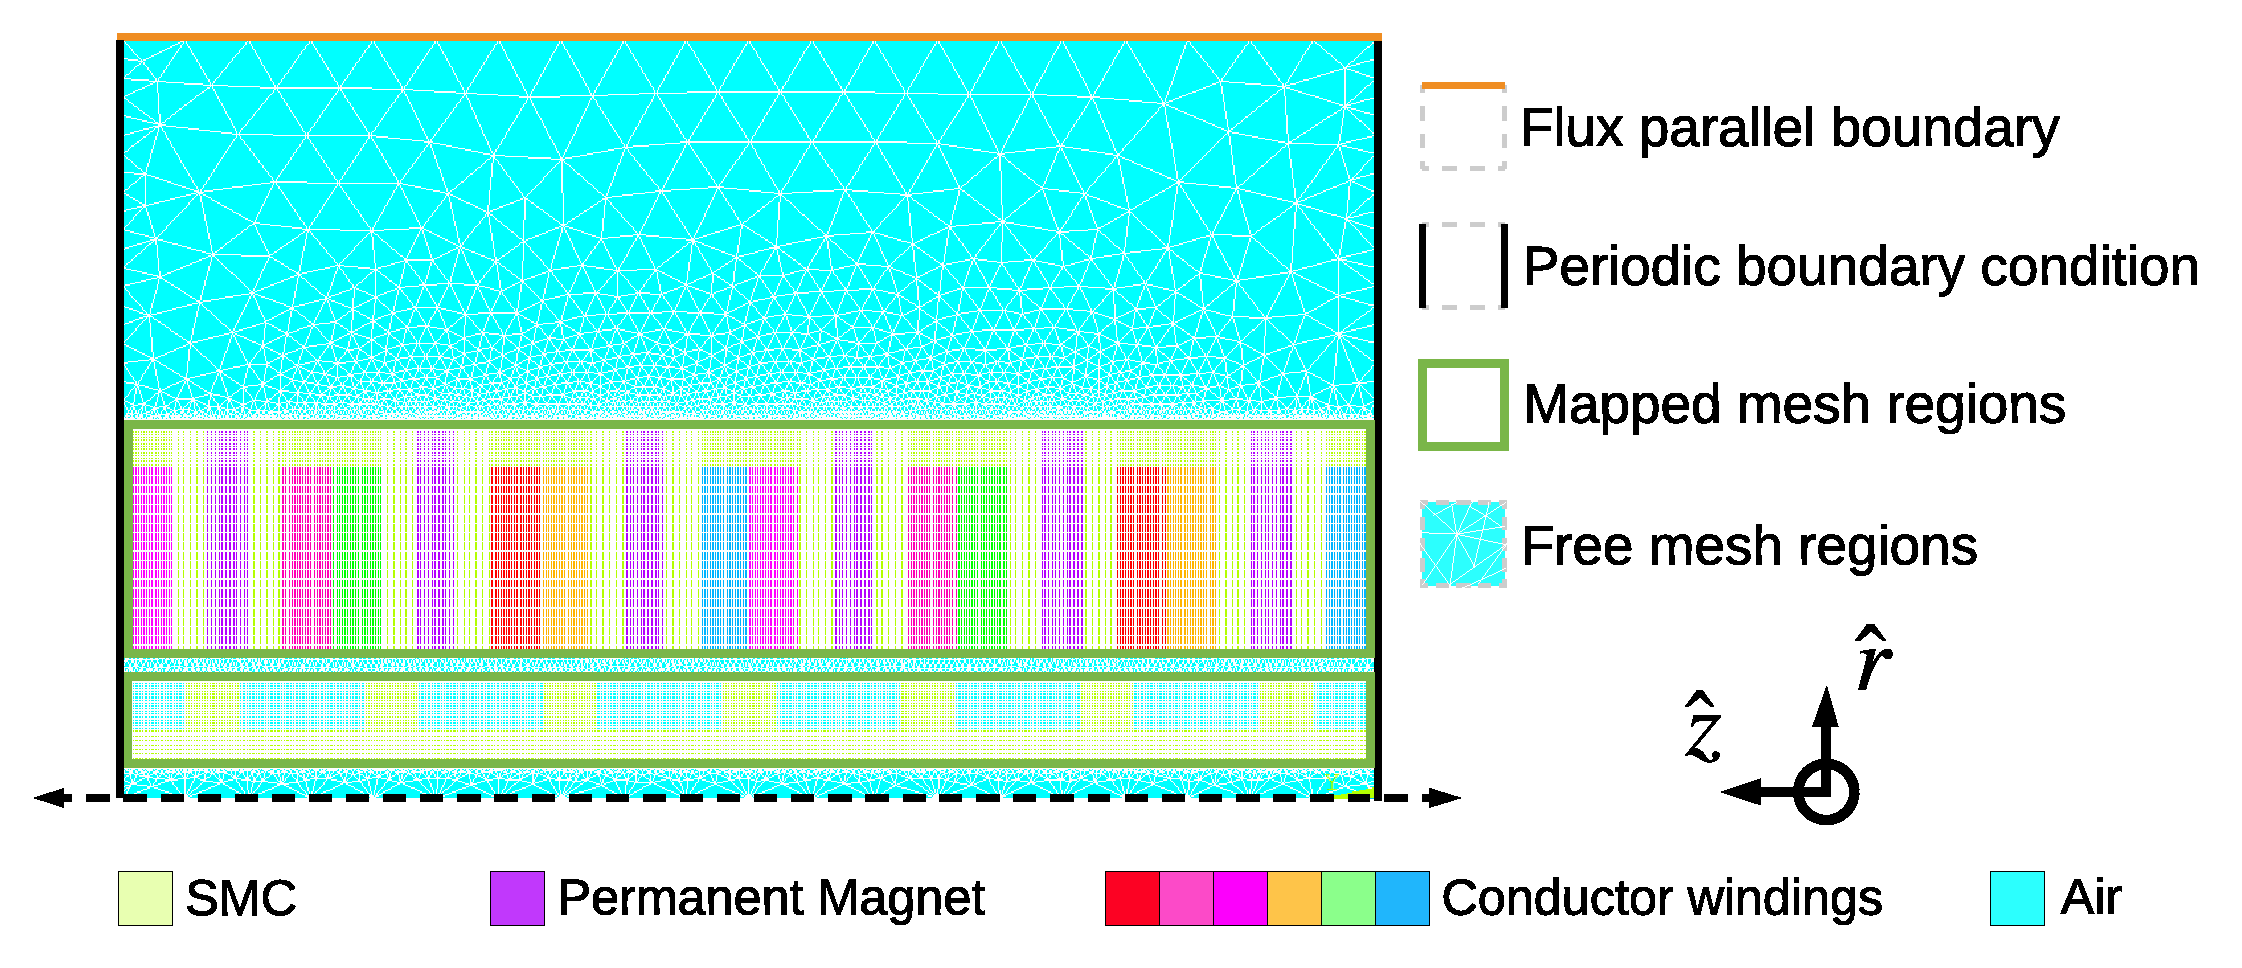
\includegraphics[width=0.98\textwidth]{chap4/images2/LFSM_periodic_setup.pdf}
                }
                \par\bigskip
                \subfloat[\label{fig:chap/rsm/LFSM/periodic_fea/thrust_waveform_study} 
                    1x motor: 
                    6 slots, 
                    7 poles, 
                    $r_{is}=\mathrm{2mm}$, 
                    $h_{R1}=\mathrm{2.4mm}$, 
                    $h_{R2}=\mathrm{6mm}$,
                    $r_{ic}=\mathrm{9.2mm}$,
                    $h_{C1}=\mathrm{12mm}$, 
                    $h_{C2}=\mathrm{15mm}$, 
                    $w_{M}=\mathrm{2.7mm}$,
                    $w_{S}=\mathrm{10.6mm}$,
                    $w_{C}=\mathrm{6.4mm}$,
                    $w_{R}=\mathrm{3.4mm}$,
                    $6\cdot L_{KC}=7\cdot L_{KS}=\mathrm{80mm}$, $\theta = 0^\circ$.
                    ]{
                    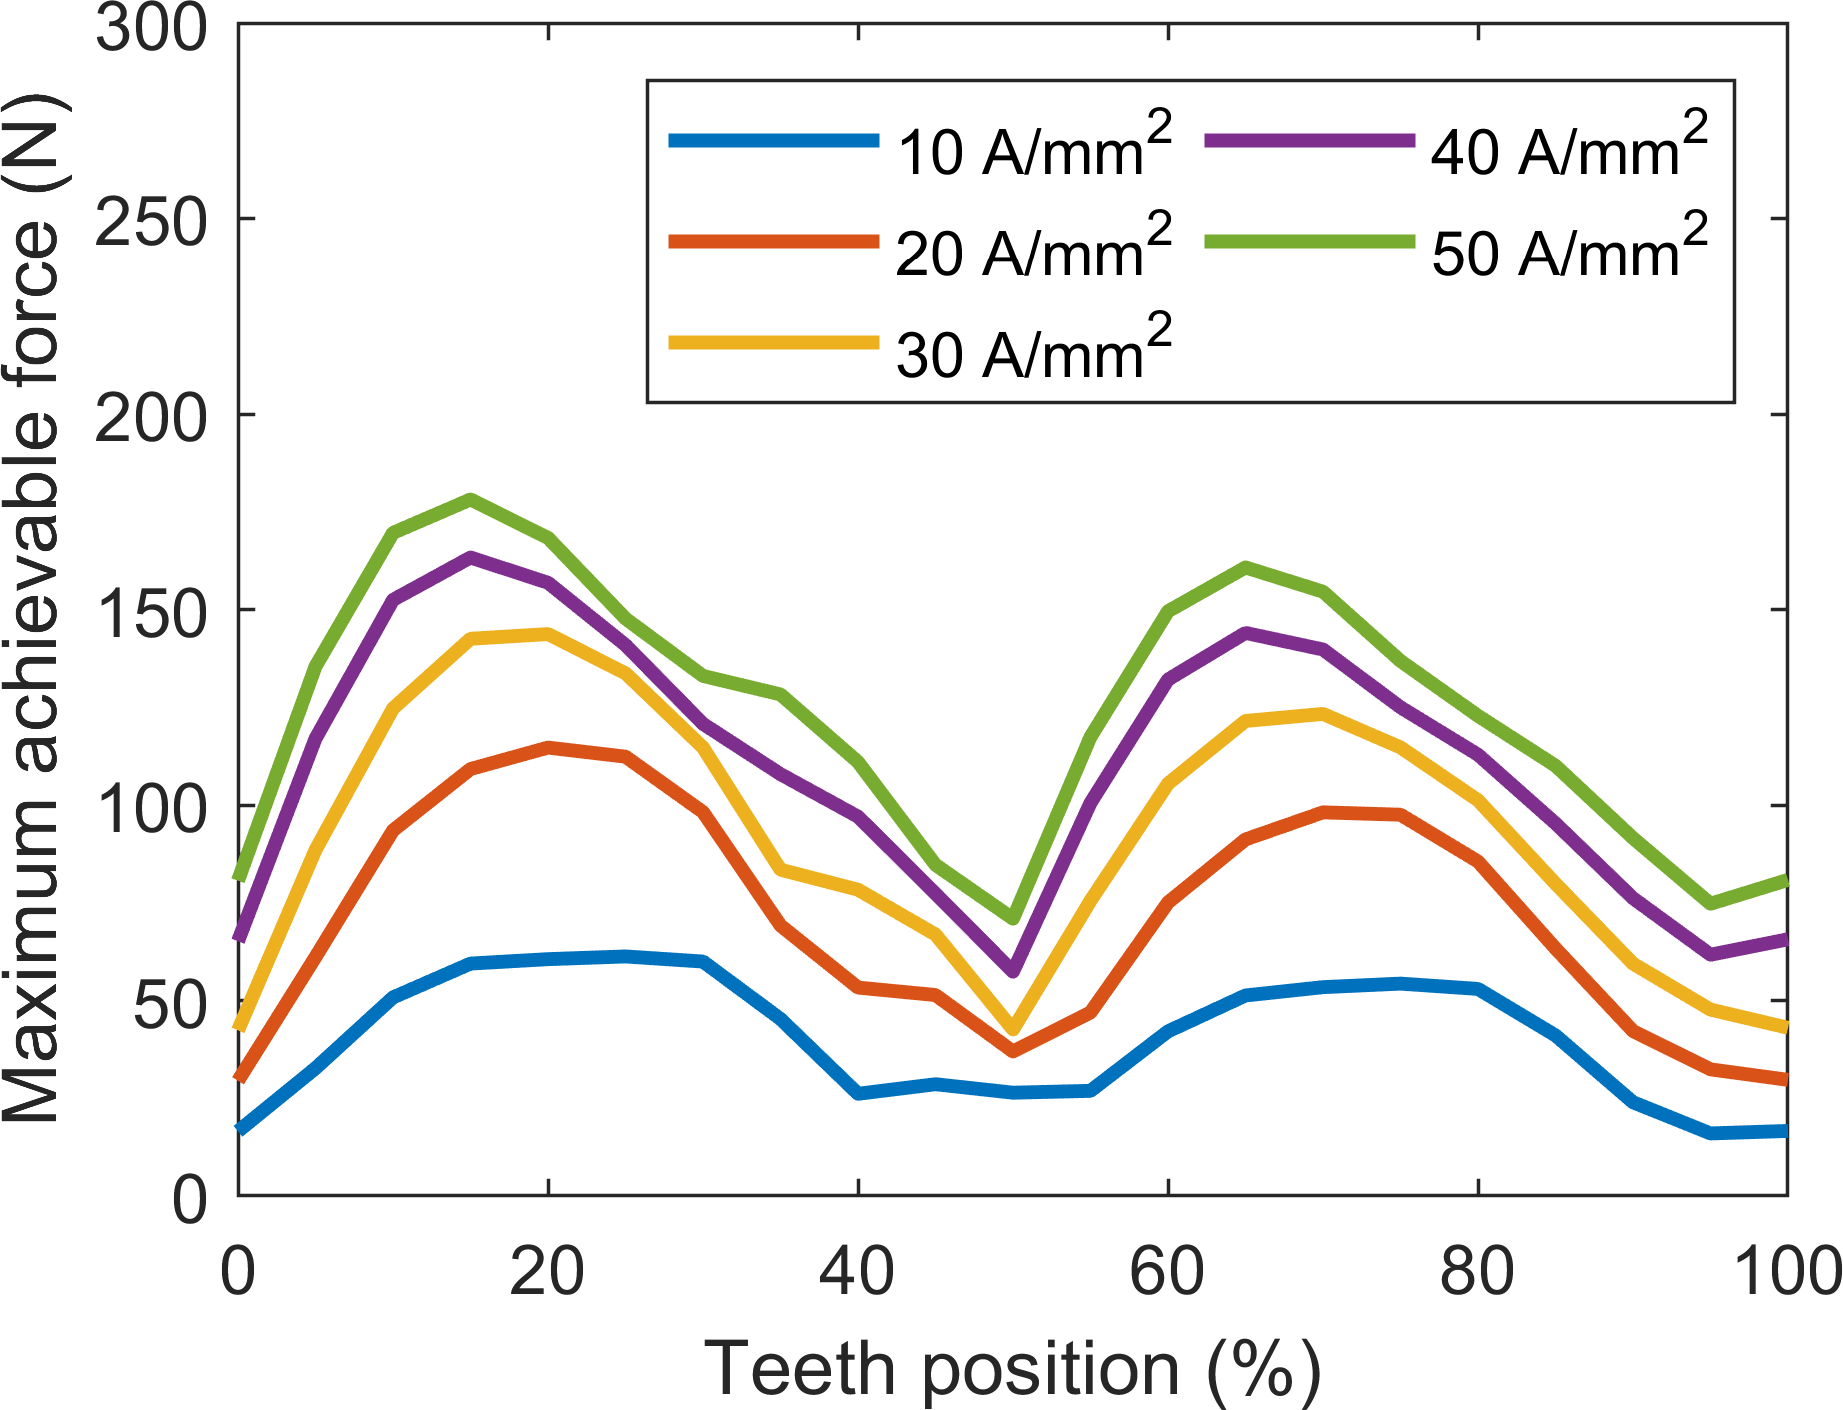
\includegraphics[width=0.45\textwidth]{chap4/images2/LFSM_thrust_waveform.png}
                }
                \,\,\,\,\,\,\,\,
                \subfloat[\label{fig:chap/rsm/LFSM/periodic_fea/scaling_study}
                    Plot of average thrust for the original motor and another motor with all dimensions doubled (``2x motor") at different current densities: $1$, $3$, $5$, $10$, $20$, $30$, $40$, and $50\,\mathrm{A/mm^2}$
                    ]{
                    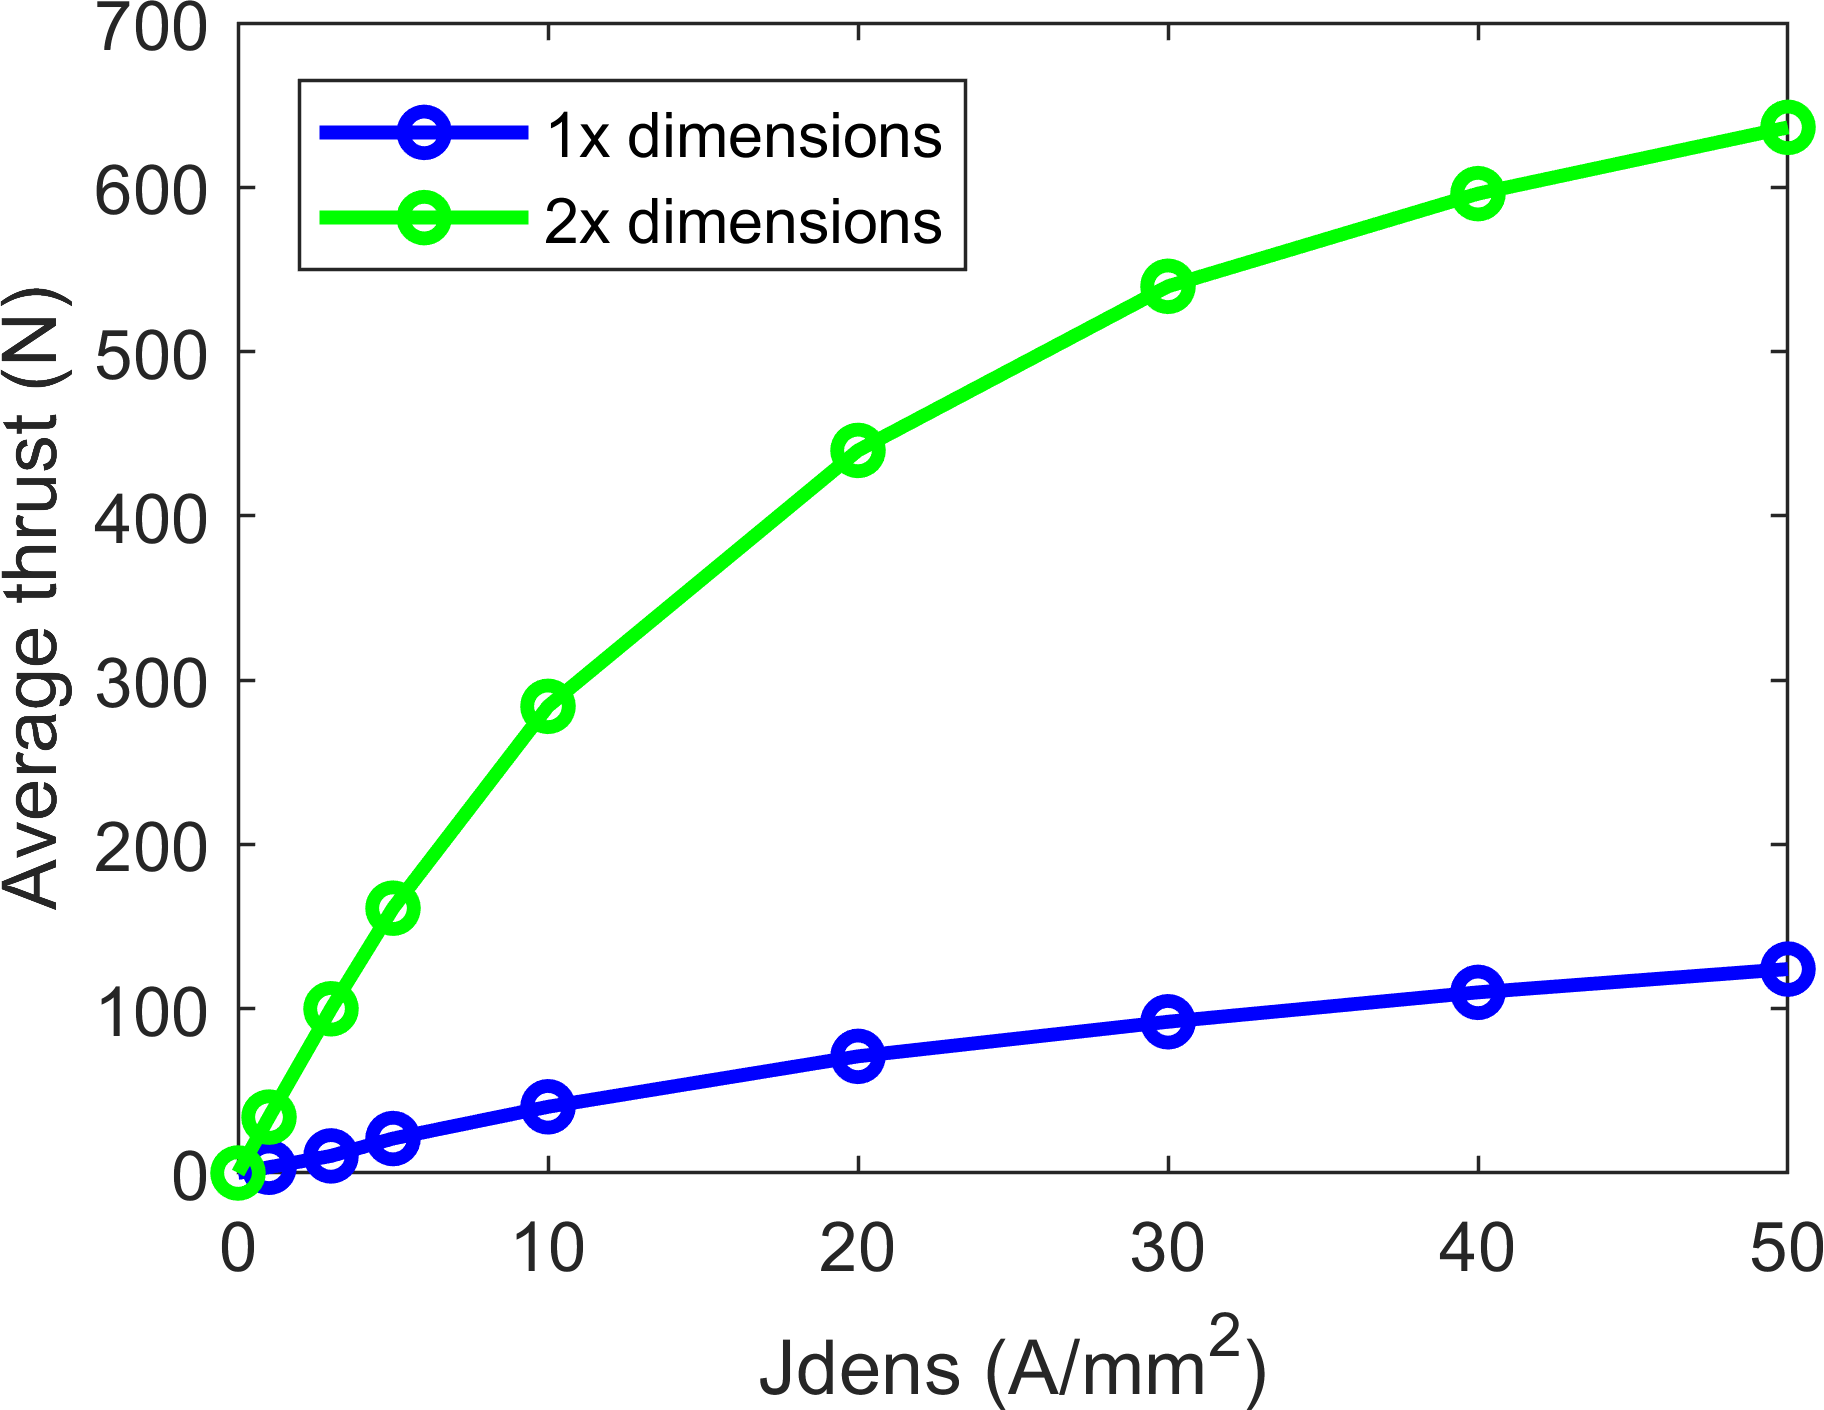
\includegraphics[width=0.45\textwidth]{chap4/images2/LFSM_scaling_effect.png}
                }
                \caption{ 
                    \label{fig:hap/rsm/LFSM/periodic_fea} The axis-symmetric \acs{FEA} model in ANSYS Mechanical APDL for evaluating force produced on the secondary $\mathrm{(a)}$. 
                    A plot of maximum achievable force at different track positions for
                    the original motor moving right $\rightarrow$ left $\mathrm{(b)}$.
                    A plot that compares the original motor's force production capability to that of a motor twice the size $\mathrm{(c)}$.
                }
            \end{figure*}
    
        
            In doubling the dimensions of a motor, the mass and volume are multiplied by a factor of $8$. Hence, when applying the same current density to the coil, the "$2\times$ motor" consumes eight times more power. For a permanent magnet motor, one would expect that the force produced would also be eight times higher, in agreement with the motor constant scaling units of $\mathrm{N/\sqrt{W\cdot kg}}$\,\cite{Ruddy2011a}. However, the scaling relationship is different in motors operating primarily on the principle of variable reluctance. The scaling difference arises because, in scaling the overall dimensions of the motor by a fixed number, the rates at which PM and winding induction lose effectiveness are different\,\cite{Melcher1981}. In a \acs{LFSM}, the thrust is produced from the flux-switching action of the armature on uni-polar flux produced by the permanent magnet\,\cite{Cheng2011}, a combination of the two operating principles. These scaling relationships apply only up to a certain power level, and above this power level, the motor performance is impacted by saturation.  
    
    
            The effect of scaling this \acs{LFSM} is shown in Fig.\,\ref{fig:chap/rsm/LFSM/periodic_fea/scaling_study}. In this particular example, for a current density up to $5\,\mathrm{A/ mm^2}$, the force produced by the "$2\times$ motor" was indeed eight times that of the original motor. This ratio dropped to seven times at $10\,\mathrm{A/ mm^2}$ and to below six times at $40\,\mathrm{A/ mm^2}$. When optimizing a motor to maximize the motor constant, one should incorporate an extra step to check whether the applied power has not exceeded the scaling relationship implied by the objective of the optimization. The motor constant $K_m$ with unit $\mathrm{N/\sqrt{W\cdot kg}}$ or $\mathrm{N/\sqrt{W}}$ cannot be used to reliably predict thrust given the input power for \acs{LFSM}. To account for the unevenness in the thrust waveform non-linearity of the power-to-thrust ratio, there required \acs{FEA} measurements of thrust at different axial offset, and at the exact power level that the optimization problem requires.
            

            The 6 slot/7 pole machine was modelled in ANSYS Mechanical APDL to measure the force generated on the secondary, as shown in Fig.\,\ref{fig:chapter/rsm/LFSM/FEA}. The 2D axis-symmetric model implemented in ANSYS  $19.2$ used a mapped mesh for the motor parts and a free mesh for the transition regions such as the air gap and the free space surrounding the structure. The periodic boundary conditions were not applied at each end of the armature repeat unit along the $\hat{z}$ direction. This setup therefore did not ignore end effects. If the ANSYS Mechanical APDL scripts were to apply the periodic boundary condition at each end of the armature, and at the same time experimented with a non-zero secondary tooth angle, the ANSYS Mechanical APDL model was tested to produce significantly more execution errors. Instead the simulation setup added three extra teeth on each end of the secondary. As the result, all simulation test cases has exactly six armature slots, and 13 teeth. Fig.\,\ref{fig:chapter/rsm/LFSM/FEA/non_periodic_FEA_setup} illustrates the new \acs{FEA} setup for the data mining step. This setup of \acs{LFSM} was chosen over the \acs{FEA} setup in Fig.\,\ref{fig:chap/rsm/LFSM/periodic_fea/fea_for_studies} because it was more robust for non-zero teeth angle $\theta$.
            

            The \acs{SMC} parts and magnets are made out of Sintex \acs{SMC} prototype materials and K$\&$J Magnetics Grade N45SH, respectively. The non-linear $\mathrm{B-H}$ relationship of the \acs{SMC} material was also fully captured in the FEA model. This setup was crucial to the design optimization process, where many different design configurations needed to be tested.
            
            
            \begin{figure*}[!ht]
                \centering
                \subfloat[\label{fig:chapter/rsm/LFSM/FEA/non_periodic_FEA_setup} A \acs{FEA} setup for mining data that is robust against non-zero teeth angle $\theta$.]{
                    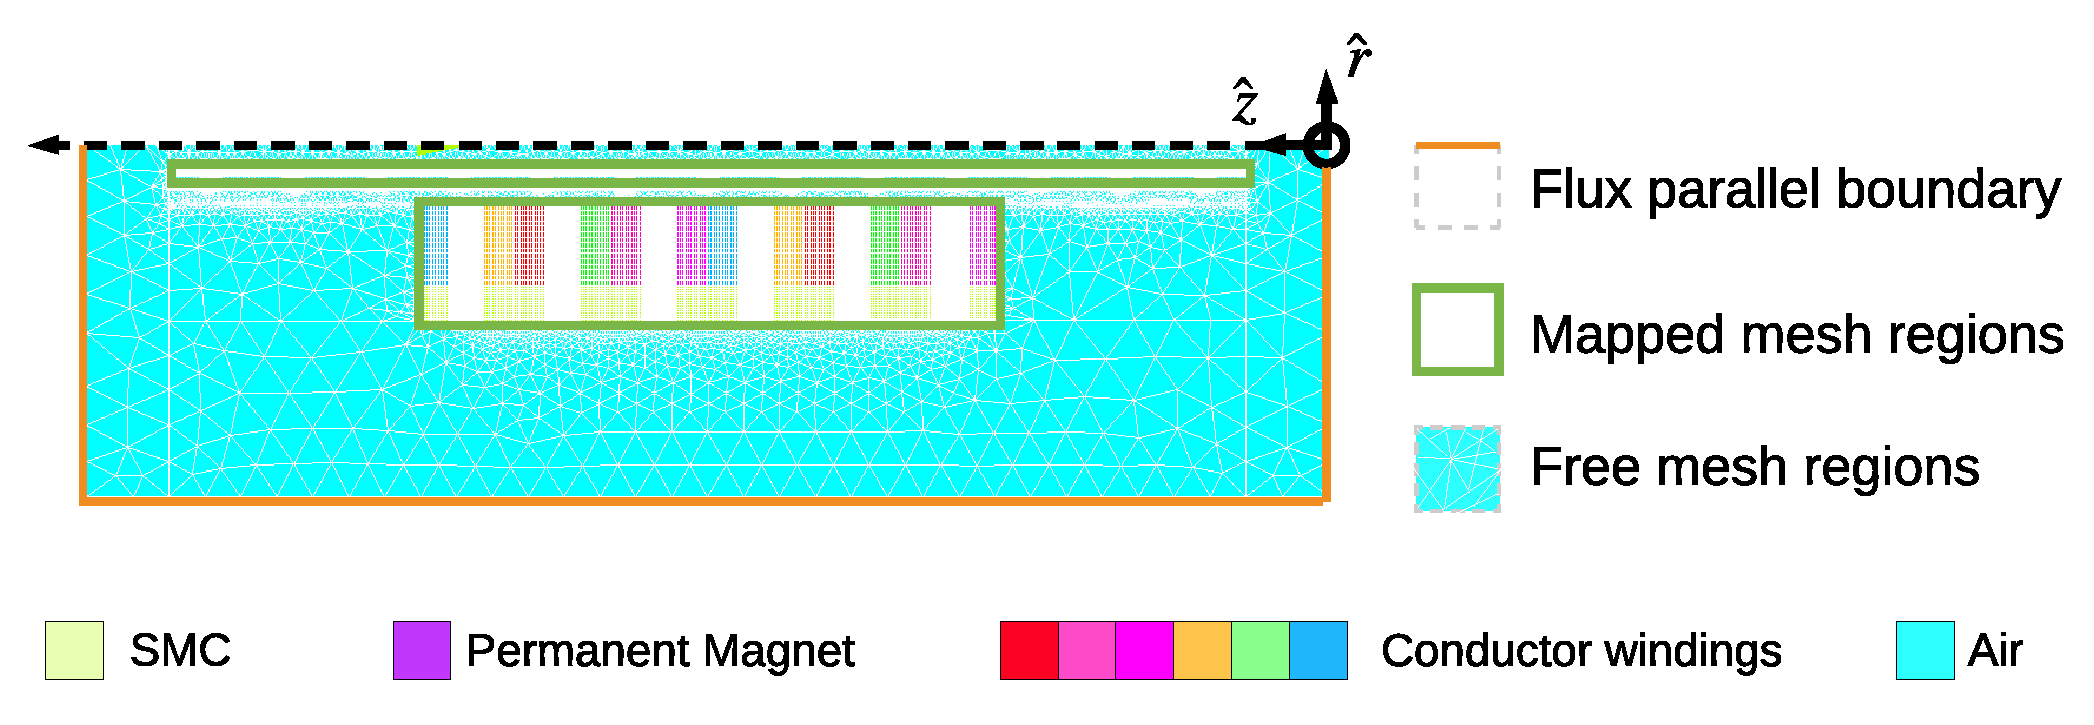
\includegraphics[width=0.98\textwidth]{chap4/images2/FEA_LFSM_non_zero_teeth.pdf}
                }
                \\
                \subfloat[\label{fig:chapter/rsm/LFSM/FEA/position 1} A \acs{FEA} mesh view of \acs{LFSM} for the beginning position]{
                    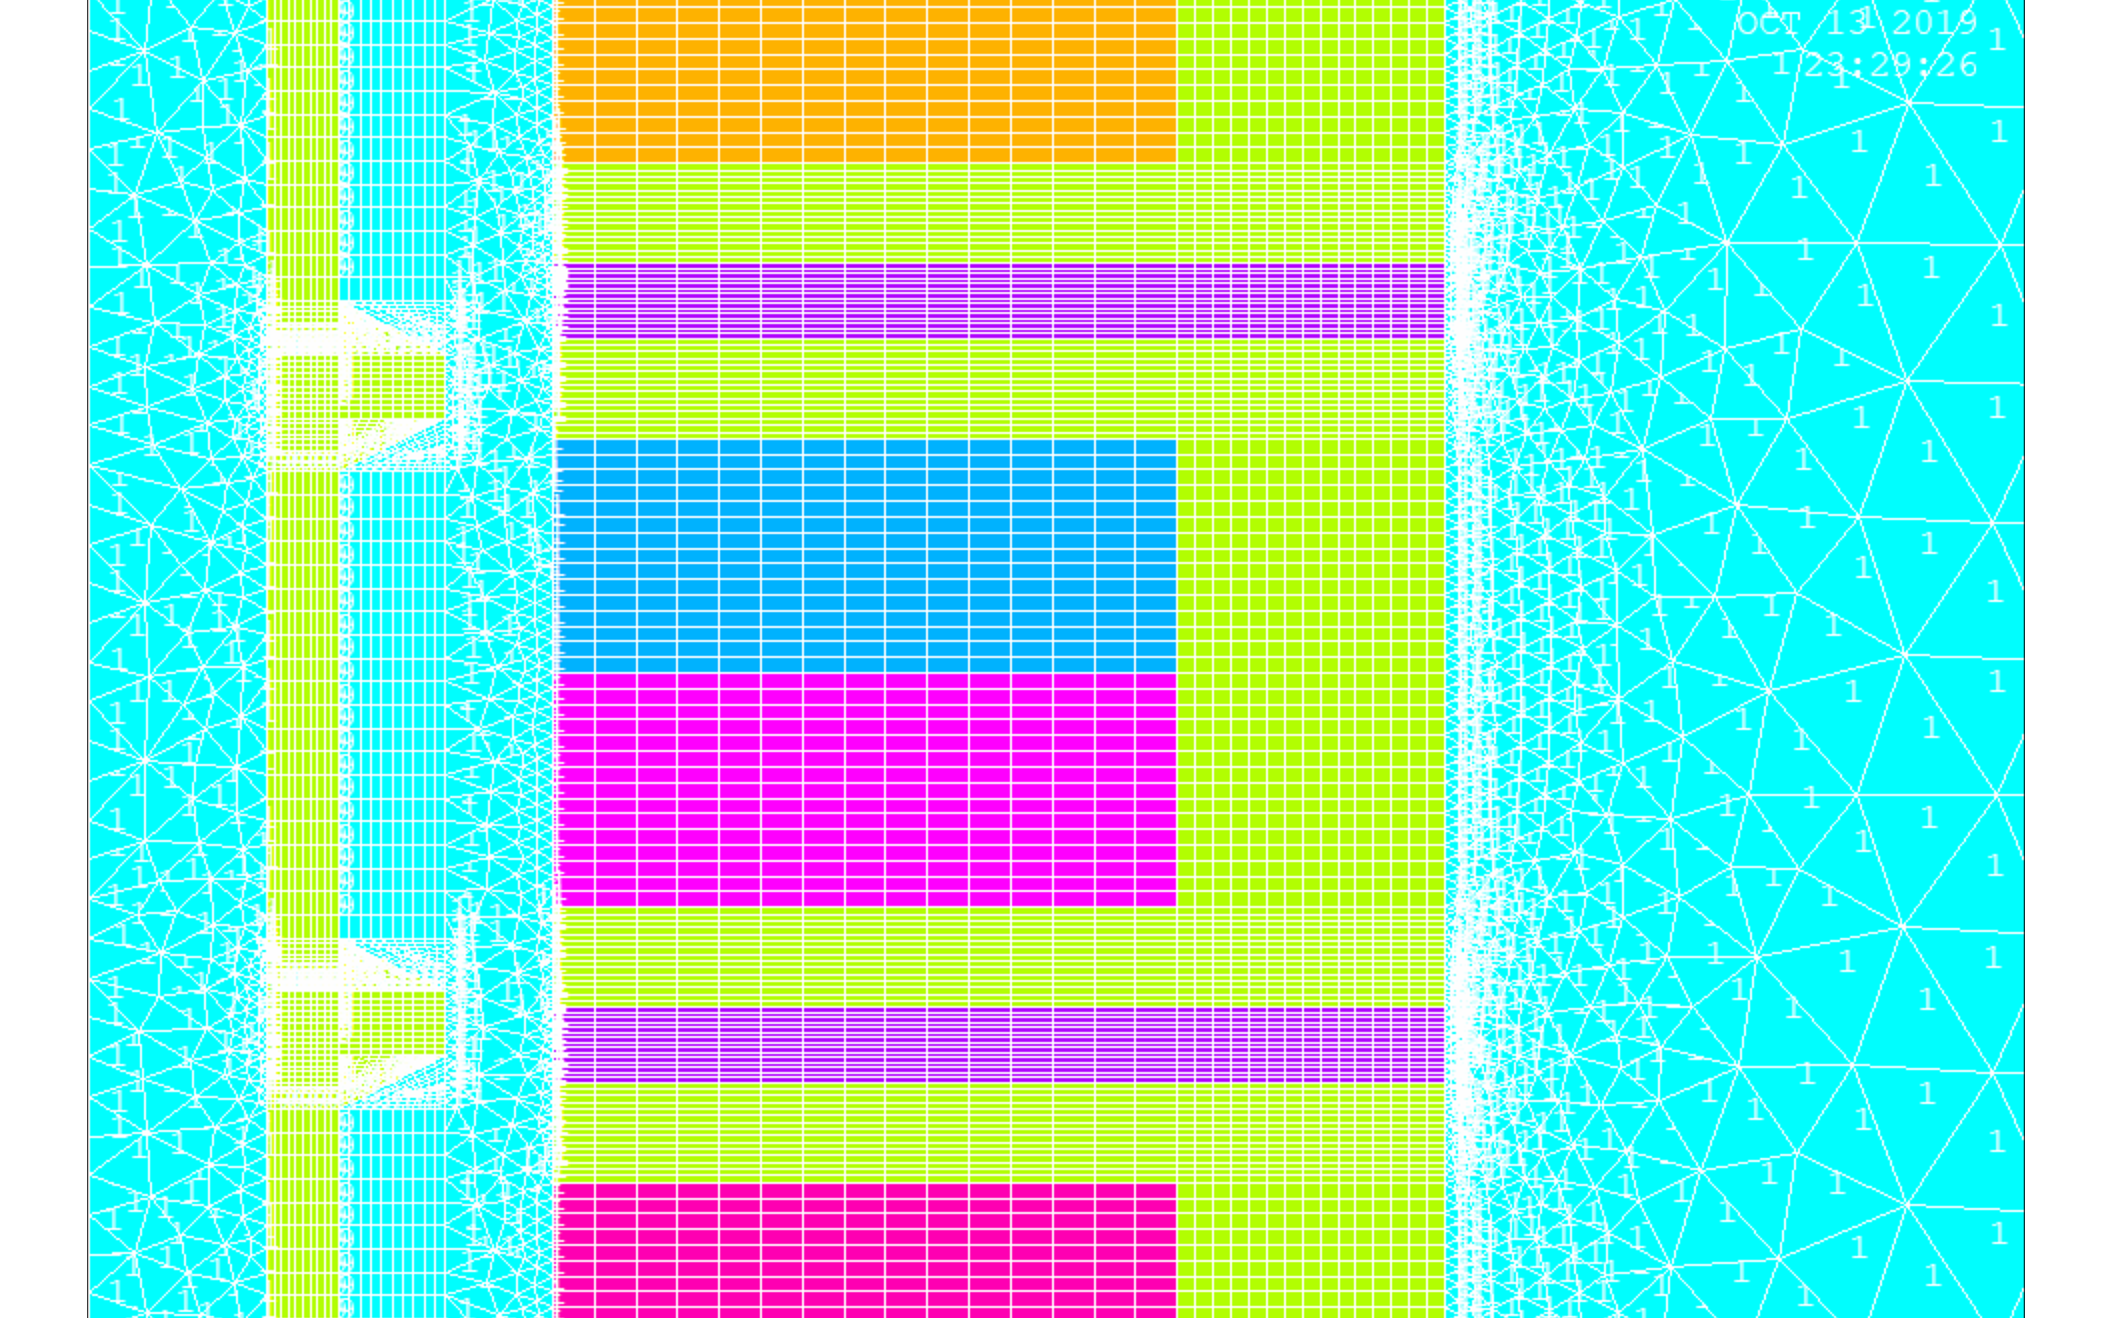
\includegraphics[width=0.45\textwidth]{chap4/images2/FEA_position_1.png}
                }
                \,\,\,\,\,\,\,\,
                \subfloat[\label{fig:chapter/rsm/LFSM/FEA/position 10} A \acs{FEA} mesh view of \acs{LFSM} for the middle position]{
                    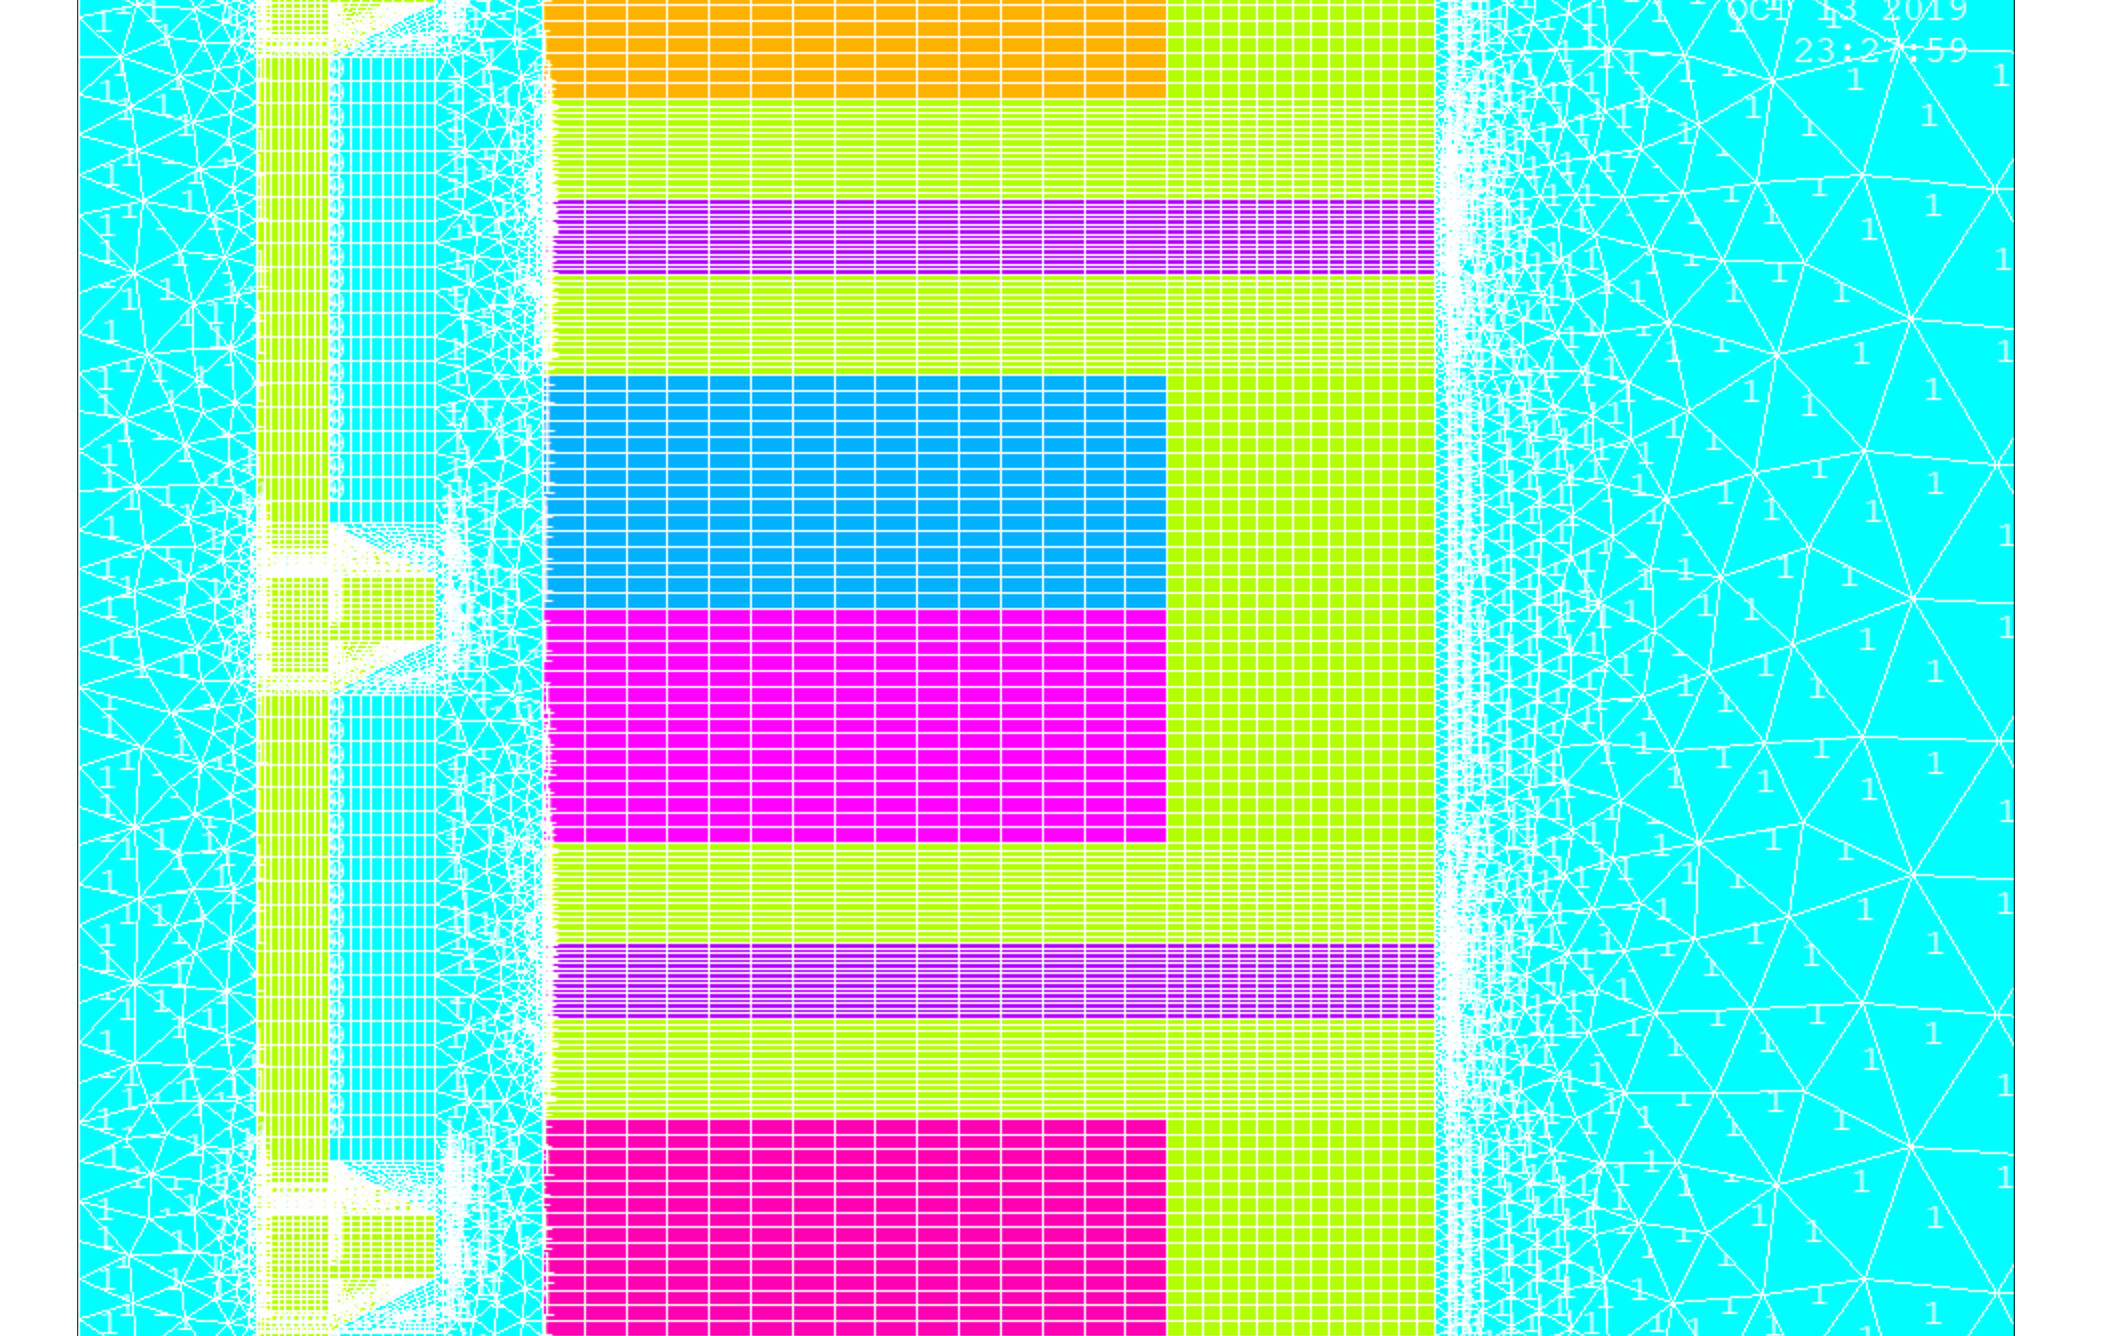
\includegraphics[width=0.45\textwidth]{chap4/images2/FEA_position_10.png}
                }
                \caption{ 
                    \label{fig:chapter/rsm/LFSM/FEA} The FEA setup for obtaining the resultant thrust given a stroke position, a 3-phase current angle, a set of design parameters, and the fixed input power. The graphics cropped from ANSYS Mechanical APDL $19.2$ shows the \acs{SMC} material in green, the free space in blue, the axial permanent magnet rings in dark purple, and the coil phases in orange and light pink.
                }
            \end{figure*}
            
            
            The base modelling script was constructed with the intention to allow for easy modification of the input parameters summarized in Table\,\ref{table:chap/rsm/LFSM/design range}. For the $56656$ motor designs, the unknowns are the cogging force, average thrust, and peak thrust at $1500\,\mathrm{W}$ input power. There were force measurements at $20$ equally spaced stroke positions and $42$ current angle offsets. Since the mesh of each simulation could be re-used for all the different current angle offsets, only the different stroke positions required re-meshing. In total, there were $1133120$ input files which represented all the unique permutations of all motor design dimensions, stroke positions, and current angle offsets. Additionally, each one of the input files contained an extra simulation at null applied current to learn about the cogging force at these various stroke positions. 
            
            
            The $1133120$ input files were sent to the \acf{HPC} infrastructure owned by the New Zealand eScience Infastructure (NeSI) for execution in parallel batches. On average, each one of the input files took $22$ minutes on a two-core Intel CPU with $3\,\mathrm{GBs}$ of RAM. The \acs{HPC} facility allowed for any user to execute $1000$ jobs in parallel. This large simulation job consumed $415506$ CPU hours and took approximately $416$ hours to complete. All verbose output of jobs was collected and doubled checked for errors and warnings, totalling $435\,\mathrm{GBs}$ of raw data in text format. The necessary information was then reduced back to $52961$ fully captured motor designs in CSV format, demonstrating a high success rate of more than $93.5\,\%$. The computed thrust output by \acs{FEA} batches was later further processed and refined into peak to peak cogging force $F_{\Delta cogging}$, average thrust $\overline{F}$, and peak thrust $F_{peak}$ for use in training the neural network.
            
            
            One additional advantage of having the data ready ahead of the optimization process is that the available data, though limited, was able provide valuable insights into identifying the principal design parameters. To investigate these hidden relationships, a co-variance heat map is plotted in Fig.\,\ref{fig:chap/rsm/LFSM/data mining/heat map}. There was a number of useful relationships identified from this heat map:
            
            
            \begin{itemize}
                \item $\alpha$ ratio can improve the average and peak thrust at the cost of more peak to peak cogging $F_{\Delta cogging}$,
                \item $r_{so}$ also improves average and peak thrust without adding more cogging, however, this inherently adds more mass,
                \item Low $\beta$ is more preferable,
                \item Surprisingly, the stator tooth design factors such as $\epsilon$ and $\delta$ have very little influence on the motor performance, even on the peak-to-peak cogging $F_{\Delta cogging}$.
            \end{itemize}
            
            
            \begin{figure}
                \centering
                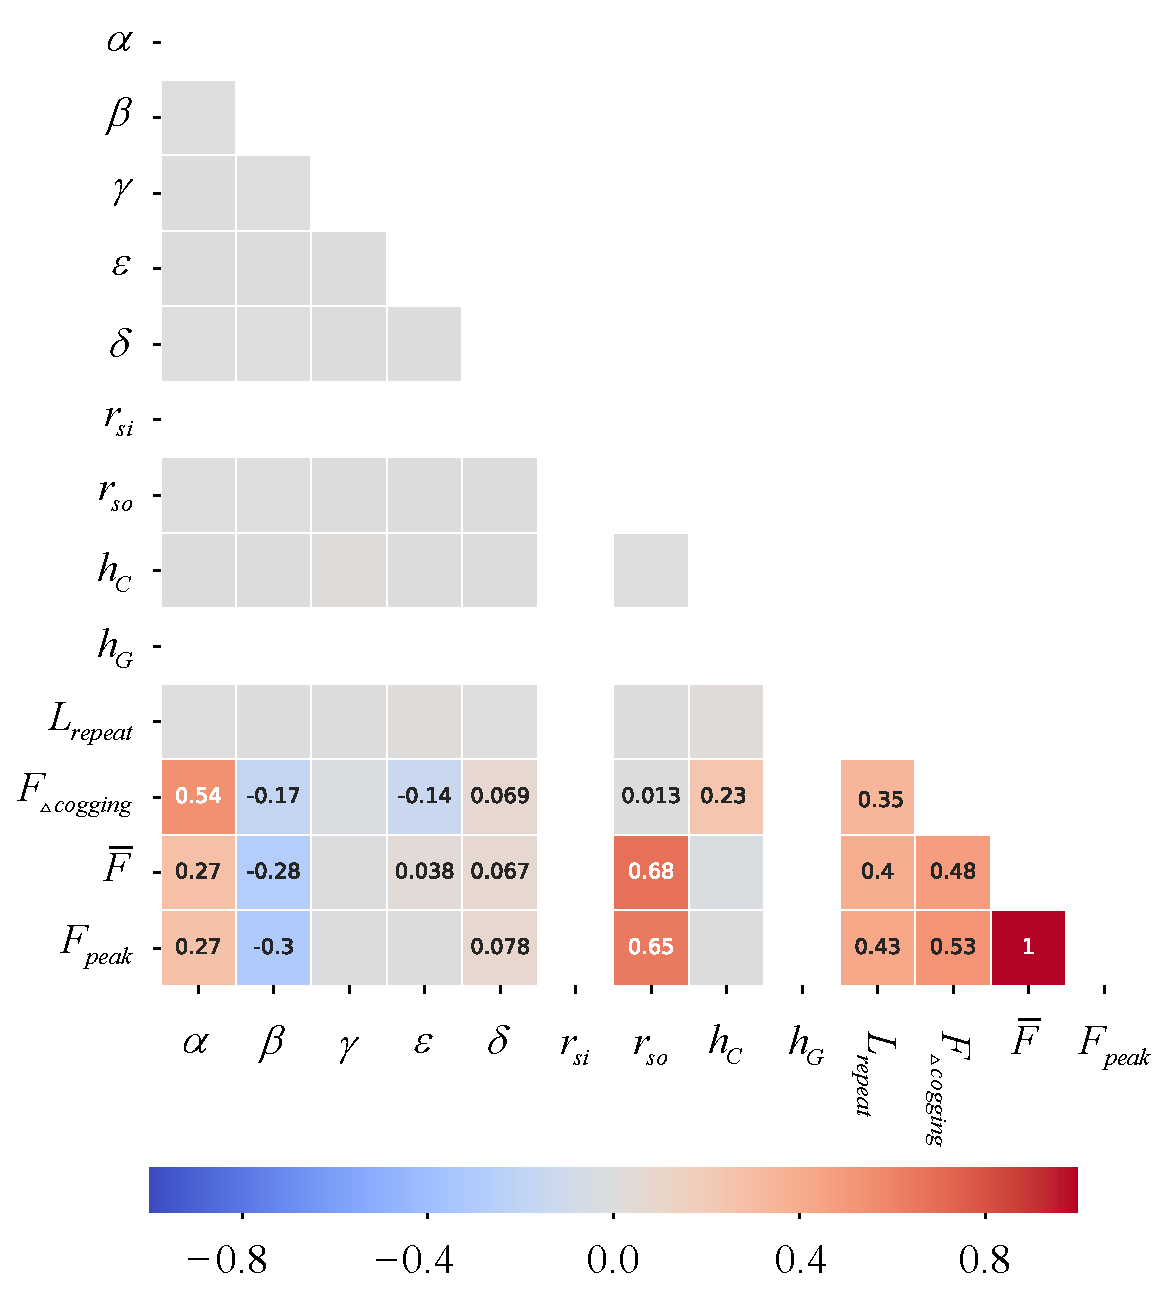
\includegraphics[width=5in, trim=0 0 0 129mm, clip]{chap4/images2/heatmap.pdf}
                \caption{A co-variance heat map which depicts the relationship between different input and output variables of the motor design data set obtained in the \acs{FEA} data mining step for \acsp{LFSM}. Red and blue on this scale mean positive and negative correlations. Small values are hidden.}
                \label{fig:chap/rsm/LFSM/data mining/heat map}
            \end{figure}
        
        
        % -----------------------------------------------------------------------------------
        % --- NEW SUB SECTION --- NEW SUB SECTION --- NEW SUB SECTION --- NEW SUB SECTION --- 
        % -----------------------------------------------------------------------------------
        \subsection{Deep regression ANN training}   \label{Chapter:RSM/LFSM/ANN training}
        
        
            \begin{figure*}
                \centering
                \subfloat[$70\%-30\%$ split model
                ]{
                    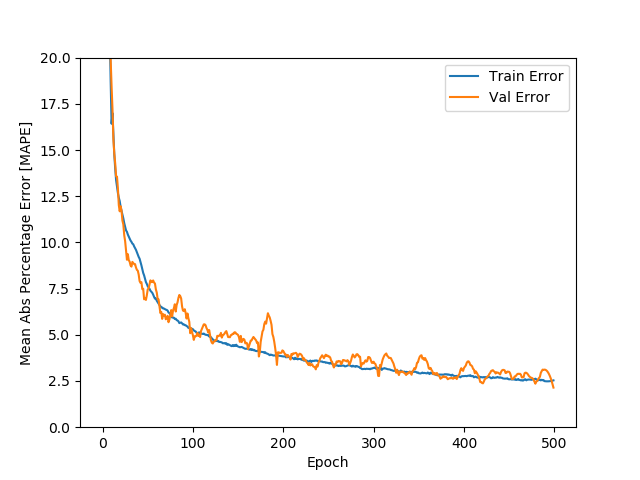
\includegraphics[width=0.5\textwidth]{chap4/images2/MAPE_MSE_6_70-30_SPLIT.png}
                    \label{fig:chapter/rsm/LFSM/training result/MAPE_70_30}
                }
                \subfloat[$75\%-25\%$ split model
                ]{
                    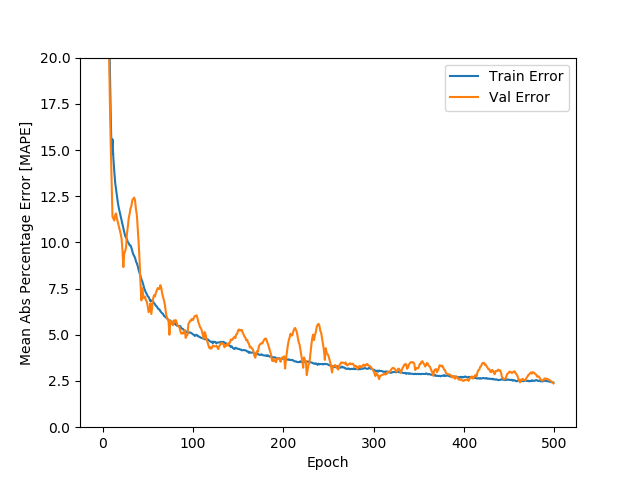
\includegraphics[width=0.5\textwidth]{chap4/images2/MAPE_MSE_6_75-25_SPLIT.png}
                    \label{fig:chapter/rsm/LFSM/training result/MAPE_75_25}
                }
                \\
                \subfloat[$80\%-20\%$ split model
                ]{
                    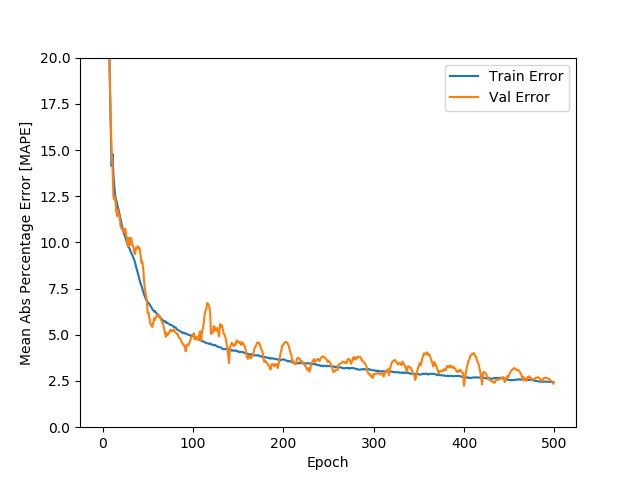
\includegraphics[width=0.5\textwidth]{chap4/images2/MAPE_MSE_6_80-20_SPLIT.png}
                    \label{fig:chapter/rsm/LFSM/training result/MAPE_80_20}
                }
                \caption{
                    Error produced by the deep learning ANN model to represent \acsp{LFSM} vs. iterations for the training data (blue) and validation data (orange). The \acs{MAPE} is plotted for the training process of (a) $70\%-30\%$, (b) $75\%-25\%$, and (c) $80\%-20\%$ models, respectively.
                }   \label{fig:chapter/rsm/LFSM/training result}
            \end{figure*}
        
        
            The data set provided both the continuous input variables (structural design factors), and the continuous output variable (thrust characteristics at a given power), which classify our application as a supervised and regression type of machine learning problem. The \acs{ANN} model was implemented in Keras and Tensorflow machine learning frameworks:

            
            \begin{itemize}
                \item Eight structural parameters were regarded as the Input Layer: $\alpha$, $\beta$, $\gamma$, $\epsilon$, $\delta$, $r_{so}$, $h_G$, and $L_{repeat}$,
                \item Three performance outputs were regarded as the Output Layer: $F_{\Delta cogging}$, $\overline{F}$, and $F_{peak}$,
                \item The $\mathrm{Adam}$ optimizer was used for \acs{ANN} training,
                \item There were six hidden layers of $256-512-512-512-512-512$ of densely connected nodes,
                \item The rectified linear unit (ReLU) activation function was used
for the input and hidden layers,
                \item The linear activation function was used for the output layer,
                \item The error to optimize for was \acs{MSE},
                \item The training and validation split were chosen at random for each of the three models are: $70\%-30\%$, $75\%-25\%$, and $80\%-20\%$,
                \item The final \acs{ANN} model was ensembled from the average of three models above.
            \end{itemize}


            After 500 training iterations, the model was shown to have a \acf{MAPE} of under $2.41\,\%$. Fig.\,\ref{fig:chapter/rsm/LFSM/training result} shows that the training and validation errors were similar, which means the deep regression model was not over-fitted to the training data set.
        
        
        % -----------------------------------------------------------------------------------
        % --- NEW SUB SECTION --- NEW SUB SECTION --- NEW SUB SECTION --- NEW SUB SECTION --- 
        % -----------------------------------------------------------------------------------
        \subsection{Optimization}                   \label{Chapter:RSM/LFSM/Optimization}
        
        
            \subsubsection{Outer Optimization}          \label{Chapter:RSM/LFSM/Optimization/Outer}
            
            
                In order to fairly compare the performance of \acsp{LFSM} to \acsp{PMLSM} in \acs{NFJI} applications, the optimization problem description needs to be simultaneously adaptable to \acsp{LFSM} and equivalent to that described in Equation\,\ref{eq:outer optimization for PMLSMs}. Note that in the previous section where the \acs{ANN} model was constructed, all designs used to construct the model were limited to a 6 slot/7 pole repeat unit. However, in the optimization problem the number of poles or \acs{SMC} teeth will need to be higher than seven in order to facilitate for the moving coil configuration. The Equation\,\ref{eq:outer optimization for LFSMs} added the last constraint to serve the said condition. The number of coil segments in a single coil repeat unit is six. To increase the number of coil phases, the mover needed to add six coil segments at a time. If more coil phases were added into a fixed length coil, the width of the individual coil winding could be found to be too small and impractical for prototyping. Therefore, the number of coil slots $N_C$ was fixed at six. This effectively made the length of coil $L_C$ the same as the repeat length $L_{repeat}$. The overall optimization for \acs{LFSM} consisted of strategic repetition of the inner optimization to maximize the average jet speed $\overline{v_{jet}}$ derived from the predicted average thrust $\overline{F}$:
                
                
                \begin{itemize}
                    \item   Limit the search to motors with a total length $L_S = L_{C} + L_{stroke}$ in between $120\,\mathrm{mm}$ and $160\,\mathrm{mm}$,
                    \item   Divide the maximum allowed motor length $L_{S-max}$ ranges into 41 equally spaced lists: $[120, 121, 122, ..., 160]\,\mathrm{mm}$ 
                    \item   Divide the coil length $L_{C}$ (equivalent to $L_{repeat}$ because $N_C$ is fixed at a value of $6$) ranges into 41 equally spaced lists:  $[50, 51, 52, ..., 90]\,\mathrm{mm}$ 
                    \item   Create a $\mathrm{2D}$ search zone for each combination of maximum motor length $L_{S-max}$ and coil mover length $L_{C}$, totalling $1681$ points,
                    \item   Run $1681$ inner optimization searches with Matlab constrained convex non-linear optimization function $fmincon()$. Details of the inner optimization will be explained below,
                    \item   Plot and identify a motor design that produces the highest average jet speed $\overline{v_{jet}}$ at the given mass constraint $M_0$.
                \end{itemize}
                
                
                \begin{equation}
                    \begin{array}{rll}
                        \textbf{minimize}       & \small{objective\,\,function}     & f(\textbf{x})=\frac{1}{v_{jet}} \\
                        \textbf{subjected to}   & \small{equality\,\,constraint}    & h_1(\textbf{x})=M - M_0= 0\\
                                                &\quad \small{where}                &\quad  M_0\in\left[325,350,375,400,425\right]\,\mathrm{g}\\
                                                &                                   & h_2(\textbf{x})=P - 1500\,\mathrm{W}=0\\
                                                &                                   & h_3(\textbf{x})=L_C - L_{C0} = 0\\
                                                &\quad \small{where}                &\quad  L_{C0}\in\left[50,51,52,...,90\right]\,\mathrm{mm}\\
                                                &                                   & h_4(\textbf{x})=V - 1\,\mathrm{mL} = 0\\
                                                & \small{inequality\,\,constraint}  & g_1(\textbf{x})=L_S-L_{S-max} \leqslant 0\\
                                                &\quad \small{where}                &\quad L_{S-max} \in \left[120,121,122,...,160\right]\,\mathrm{mm} \\
                                                & \small{other\,\,constraints}       & N_C, N_S \in 	\mathbb{N} \\ 
                                                &\quad \small{where}                &\quad N_C = 6\\
                                                &                                   &\quad N_S \geq 8
                                                \\ \\
                    \end{array}
                    \label{eq:outer optimization for LFSMs}
                \end{equation}
                
                
                
                Given each combination of coil length $L_{C}$ and maximum motor length $L_{S-max}$, the maximum number of whole stator \acs{SMC} teeth $N_S$, the corresponding stator length $L_S$ that can be fitted, and the stroke length $L_{stroke}$ can be derived by the following equations:


                \begin{equation}
                    N_S = \bigg\lfloor  \frac{L_{S-max}}{L_C} \cdot 7 \bigg\rfloor
                    \label{eq:max mumber of teeth for LFSM stator}
                \end{equation}
                
                
                \begin{equation}
                    L_S = {\bigg\lfloor  \frac{L_{S-max}}{L_C} \cdot 7 \bigg\rfloor} \frac{L_C}{7}
                    \label{eq:possible stator length LFSM stator}
                \end{equation}
                
                
                \begin{equation}
                    L_{stroke} = {\bigg\lfloor  \frac{L_{S-max}}{L_C} \cdot 7 \bigg\rfloor} \frac{L_C}{7} - L_C
                    \label{eq:possible stroke length LFSM stator}
                \end{equation}
                
                
                Together with the predicted thrust $F$, ampoule volume $V$, and water density $\rho_w$, the jet velocity $v_{jet}$ can be derived directly from Equation\,\ref{eq:power dissipation for PMLSMs}:
            
            
                \begin{equation}
                    v_{jet} = \sqrt[4]{\frac{4 F {L_{stroke}}^2}{\rho_w V^2}}
                    \label{eq:v_jet for FSM}
                \end{equation}
                
                
            \subsubsection{Inner Optimization}          \label{Chapter:RSM/LFSM/Optimization/Inner}
                
                
                \begin{figure*}
                  \centering
                  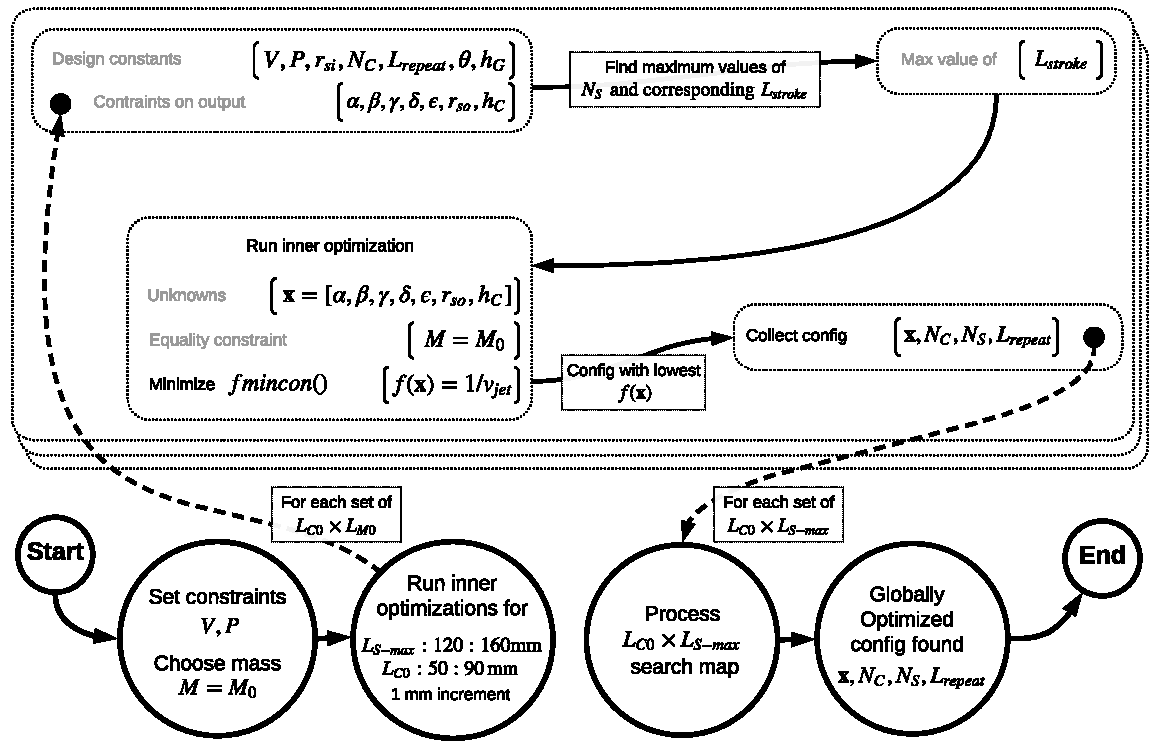
\includegraphics[width=5.9in]{chap4/images2/RSM_LFSM_optimization.pdf}
                  \caption{Summary of the top-level motor optimization algorithm and inner optimization routine for \acsp{LFSM}. The algorithm uses motor specifications $V$, $P$, $M$ to determine the motor parameters $\textbf{x}=[\alpha,\beta,\gamma,\delta,\epsilon,r_{so},h_C]$, $N_C$, $N_S$, $L_{repeat}$ at which the jet speed $v_{jet}$ can be maximized.}
                  \label{fig:chapter/rsm/fsm/top level optmization}
                \end{figure*}
                
                
                From a bird eye view, the outer optimization loop provided unique combinations of $L_{C0}$, $L_{S-max}$, and $M_0$ to produce a value of $L_C$, as well as sensible values for $N_S$ and $L_{stroke}$ explained in Equations\,\ref{eq:max mumber of teeth for LFSM stator} and \ref{eq:possible stroke length LFSM stator}. At each point in the $L_{C0} \times L_{S-max}$ space, multiple inner optimizations performed a non-linear constraint optimization for the unknown variables vector $\textbf{x}$:
            
            
                \begin{equation}
                    \textbf{x} = \left[ \alpha,\beta,\gamma,\delta,\epsilon,r_{so},h_{C} \right]
                    \label{eq:inner optimization x of FSM}
                \end{equation}
                
                
                The tooth angle $\theta$ was fixed at $\arctan(1/2)$ to simplify the problem. Other constants such as the inner radius of the stator $r_{si}$, and the mover-stator air gap $h_G$ were made equal to \acsp{PMLSM} inner magnet radius $r_{mi}$, and magnet-coil gap $gap_{mc}$, respectively. The constraints on the input parameters strictly followed the parameter ranges established in Table\,\ref{table:chap/rsm/LFSM/design range} with the only difference of having the value of $N_S$ starting from eight and upward to facilitate for a non-zero stroke length $L_{stroke}$. The inner and outer optimization unknown constraints for \acs{LFSM} are summarized in Table\,\ref{table:chap/rsm/LFSM/optimization unknown constraints}.
                
                
                \begin{table}[!ht]
                    \renewcommand{\arraystretch}{1.2}
                    \caption{Summary of the inner and outer optimization constraints for \acs{LFSM}}
                    \label{table:chap/rsm/LFSM/optimization unknown constraints}
                    \centering
                    \begin{tabular}{@{}llr@{}}
                    \hline
                    \bfseries Parameter & \bfseries Description & \bfseries Values\\
                    \hline
                        $\alpha$	    & Ratio of $w_M$ over $L_{KC}$              &	$0.1-0.4$\\ 
                        $\beta$	        & Ratio of $w_C$ over $w_S$		            &	$0.4-0.9$\\ 
                        $\gamma$	    & Ratio of $h_{CM}$ over $h_C$			    &	$0.6-0.9$\\ 
                        $\delta$	    & Ratio of $w_R$ or $L_{KS}$		        &	$0.1-0.3$\\ 
                        $\epsilon$	    & Ratio of $h_{R1}$ or $h_{R2}$		        &	$0.4-0.6$\\ 
                        $r_{so}$	    & Outer radius of SMC stator core 			&	$4-10\,\mathrm{mm}$\\ 
                        $h_C$           & Thickness of the mover assembly           &	$5-30\,\mathrm{mm}$\\ 
                    \hline
                        $N_C$	        & Number of armature slots 		            &	$6$\\ 
                        $N_S$	        & Number of mover pole 		                &	$\geq 8$\\ 
                        $L_{C0}$	    & Length of coil equality constraint		&	$50-90\,\mathrm{mm}$\\ 
                        $L_{S-max}$	    & Length of stator inequality constraint	&	$120-160\,\mathrm{mm}$\\
                    \hline  \\
                    \end{tabular}
                \end{table}    
                
                
                Each inner optimization aimed at finding $\textbf{x}$ given $[N_C, L_{repeat}, L_{S-max}]$. Each first attempted to find the maximum value of $L_{stroke}$ while rounding down the number of stator teeth $N_S$. The routine then worked to define the unknown $\textbf{x}$ in order to maximize the jet speed $v_{jet}$ with the unknown variable ranges summarized in Table\,\ref{table:chap/rsm/LFSM/optimization unknown constraints}. Additionally, the optimization description in Equation\,\ref{eq:inner optimization for PMLSMs} was applicable for the inner optimization of \acs{LFSM}. The mass term $M$ was obtained via the following set of equations:
                
                
                \begin{equation}
                    w_M = \frac{\alpha}{N_C} L_{repeat}
                    \label{eq:rsm/LFSM/w_m}
                \end{equation}
                
                
                \begin{equation}
                    w_C = \beta\bigg(\frac{L_{repeat}}{N_C}-w_M\bigg);
                    \label{eq:rsm/LFSM/w_c}
                \end{equation}
                
                
                \begin{equation}
                    w_{smc-top} = \frac{1-\beta}{2}\bigg(\frac{L_{repeat}}{N_C}-w_M\bigg)
                    \label{eq:rsm/LFSM/w_smc_top}
                \end{equation}
                
                
                \begin{equation}
                    w_{smc-bot} =  \frac{\delta }{N_S}L_{repeat}
                    \label{eq:rsm/LFSM/w_smc_bot}
                \end{equation}
                
                
                \begin{equation}
                    h_{smc} = r_{oc} - r_{mc}
                    \label{eq:rsm/LFSM/h_smc}
                \end{equation}
                
                
                \begin{equation}
                    \begin{array}{c}
                        V_{stator-repeat} = \pi \bigg[  L_{repeat}  \big({r_{ms}}^2-{r_{is}}^2\big)\\
                        + N_S  \big(r_{os}-r_{ms}\big)\,\tan{\theta}\,\big({r_{os}}^2-{r_{ms}}^2\big)\\
                        + N_S\,w_{smc-bot}\big( {r_{so}}^2 - {r_{ms}}^2 \big)\bigg]
                    \end{array}
                    \label{eq:rsm/LFSM/V_stator_repeat}
                \end{equation}
                
                
                \begin{equation}
                    V_{stator} = \frac{N_S}{N_C}V_{stator-repeat}
                    \label{eq:rsm/LFSM/V_stator}
                \end{equation}
                
                
                \begin{equation}
                    V_{conductor} = \pi\,N_C\,w_c\,\big( {r_{mc}}^2-{r_{ic}}^2 \big)
                    \label{eq:rsm/LFSM/V_conductor}
                \end{equation}
                
                
                \begin{equation}
                    V_{magnet} = \pi\,N_C\,w_m\,\big( {r_{oc}}^2-{r_{ic}}^2 \big)
                    \label{eq:rsm/LFSM/V_magnet}
                \end{equation}
                
                
                \begin{equation}
                    V_{smc-mover} = 2\,\pi\,N_C\,w_{smc-top}\,\big( {r_{mc}}^2-{r_{ic}}^2 \big) + \pi \big( L_{repeat}-N_C w_m \big) \big( {r_{oc}}^2-{r_{mc}}^2 \big) 
                    \label{eq:rsm/LFSM/V_smc_mover}
                \end{equation}
                
                
                \begin{equation}
                    M= V_{stator}\,\rho_{smc} + V_{conductor} \big(0.6\,\rho_c + 0.4\,\rho_{ins} \big) + V_{magnet}\,\rho_{m} + V_{smc-mover}\,\rho_{smc}
                    \label{eq:rsm/LFSM/M}
                \end{equation} \\
                
                
                where the copper fill factor was $60\%$, and material densities $\rho_{smc}$, $\rho_c$, $\rho_{ins}$, $\rho_{m}$ were $7500\,\mathrm{kg/m^3}$, $8920\,\mathrm{kg/m^3}$, $1350\,\mathrm{kg/m^3}$, $7600\,\mathrm{kg/m^3}$, respectively. 
                
                
                Similar to the inner optimizations of \acsp{PMLSM} in Section\,\ref{Chapter:PMLSM design HM/design optimization/optimization formulation/inner} and Section\,\ref{Chapter:RSM/PMLSM/Optimization}, the inner optimization here used constrained nonlinear multi-variable optimization based on the interior point algorithm (MATLAB Optimization Toolbox) to minimize the objective function in Equation\,\ref{eq:inner optimization for PMLSMs}. It should be noted that each objective function evaluation required a prediction of $v_{jet}$, which was inferred by the \acs{ANN} model described in Section\,\ref{Chapter:RSM/LFSM/ANN training}. The method at which the \acs{ANN} was inferred is depicted in Fig.\,\ref{fig:chapter/rsm/PMLSM/inference options/web services}. Upon finishing the inner optimizations for each pair $L_{C0} \times L_{S-max}$, the control flow saved the best performing motor configuration and moved on to the next $L_{C0} \times L_{S-max}$. Fig.\,\ref{fig:chapter/rsm/fsm/top level optmization} summarizes and illustrates both the outer and the inner optimization algorithms.
                
                
                
                
                    

        % -----------------------------------------------------------------------------------
        % --- NEW SUB SECTION --- NEW SUB SECTION --- NEW SUB SECTION --- NEW SUB SECTION --- 
        % -----------------------------------------------------------------------------------
        \subsection{Results}                   \label{Chapter:RSM/LFSM/Results}        
                
            With the objective function evaluation using \acs{ANN} models at its core, the global optimization results of \acs{LFSM} were collected and summarized in Table\,\ref{table:chap/rsm/LFSM/result for global optimization of FSM via RSM method}. The table shows the optimization results for different motor mass constraints $M0 = [325, 350, 375, 400, 425]\,\mathrm{g}$.
            
            
            Looking at one specific result for the global optimization of constraints set $P=1500\,\mathrm{W}$, $V=1\,\mathrm{mL}$, $r_{si}=2\,\mathrm{mm}$, $h_G=1.2\,\mathrm{mm}$, $N_C=6$, $M_0=325\,\mathrm{g}$, $\theta = \arctan{1/2}$ on the search space $L_{C0}:50-90\,\mathrm{mm}$, and $L_{S-max}:120-160\,\mathrm{mm}$, the algorithm found an under-hung \acs{LFSM} with $\alpha=0.36$, $\beta=0.44$, $\gamma=0.63$, $\delta=0.20$, $\epsilon=0.50$, $r_{so}=8.11\,\mathrm{mm}$, $h_C=5.37\,\mathrm{mm}$, $N_S=17$, $L_S=167.86\,\mathrm{mm}$, and $L_{stroke}=92.86\,\mathrm{mm}$. The motor is able to theoretically produce an average thrust $\overline{F} = 129.01\,\mathrm{N}$ and an average jet speed $\overline{v_{jet}}=154.79\,\mathrm{m/s}$. The achievable jet speed was reasonably far from $200\,\mathrm{mm}$, which is known as the jet speed required to guarantee a \acs{NFJI} delivery. 
            
            
            If we now adjust the radius of the drug ampoule so that the average jet speed can reach $200\,\mathrm{m/s}$, the maximum drug volume $V$ can be delivery is now $V_{new}=0.60\,\mathrm{mL}$. This conversion was explained in Equations\,\ref{eq:v_jet and V} and \ref{eq:v_jet and V ratio}. For the optimized motor configurations obtained at mass $M$ of $350\,\mathrm{g}$, $375\,\mathrm{g}$, $400\,\mathrm{g}$, $425\,\mathrm{g}$, the corresponding average jet speed $\overline{v_{jet}}$ are $159.16\,\mathrm{m/s}$, $164.00\,\mathrm{m/s}$, $168.38\,\mathrm{m/s}$, $172.27\,\mathrm{m/s}$, respectively. The reduced volume $V_{new}$ for these motors are $0.63\,\mathrm{mL}$, $0.67\,\mathrm{mL}$, $0.71\,\mathrm{mL}$, and $0.74\,\mathrm{mL}$, in the same order. Fig.\,\ref{fig:chapter/rsm/LFSM/optimization search space result for differnt mass} provides global optimization plots of $\overline{v_{jet}}$ for the search space $L_{S-max}:120\,\mathrm{mm}\rightarrow 160\,\mathrm{mm} \times L_{C0}:50\,\mathrm{mm}\rightarrow 90\,\mathrm{mm}$ using $P=1500\,\mathrm{W}$, $V=1\,\mathrm{mL}$, $r_{si}=2\,\mathrm{mm}$, $h_G=1.2\,\mathrm{mm}$, $N_C=6$, $M_0=325\,\mathrm{g}$, $\theta = \arctan{1/2}$ and $M_0=[325,350,375,400,425]\,\mathrm{g}$. 
 
            
            \begin{landscape}
                \begin{table}
                    \renewcommand{\arraystretch}{1.2}
                    \caption{Summary of \acs{LFSM} design optimization values and performance using \acs{RSM} method}
                    \label{table:chap/rsm/LFSM/result for global optimization of FSM via RSM method}
                    \centering
                    \begin{tabular}{lllrrrrr}
                        \hline
                        \textbf{Params}     & \textbf{Description}                            & \textbf{Unit}           & $M_0=\mathbf{325\,g}$ & $\mathbf{350\,g}$ & $\mathbf{375\,g}$ & $\mathbf{400\,g}$ & $\mathbf{425\,g}$ \\
                        \hline
                        $P$                  & Fixed electrical power input              & $\mathrm{kW}$  & 1.50           & 1.50           & 1.50           & 1.50           & 1.50           \\
                        $V$                  & Volume of NFJI drug ampoule               & $\mathrm{mL}$  & 1.00           & 1.00           & 1.00           & 1.00           & 1.00           \\
                        \hline
                        $L_{C0:optim}$       & Inner loop's $L_C$ at global optimum      & $\mathrm{mm}$  & 65.00          & 62.00          & 70.00          & 70.00          & 70.00          \\
                        $L_{S-max:optim}$    & Inner loop's $L_S$ at global optimum      & $\mathrm{mm}$  & 160.00         & 160.00         & 90.00          & 90.00          & 90.00          \\
                        $\alpha$             & Ratio of $w_M$ over $L_{KC}$              &                & 0.36           & 0.33           & 0.34           & 0.33           & 0.33           \\
                        $\beta$              & Ratio of $w_C$ over $w_S$                 &                & 0.44           & 0.46           & 0.47           & 0.48           & 0.46           \\
                        $\gamma$             & Ratio of $h_{CM}$ over $h_C$              &                & 0.63           & 0.65           & 0.65           & 0.64           & 0.64           \\
                        $\delta$             & Ratio of $w_R$ or $L_{KS}$                &                & 0.20           & 0.18           & 0.19           & 0.18           & 0.19           \\
                        $\epsilon$           & Ratio of $h_{R1}$ or $h_{R2}$             &                & 0.50           & 0.50           & 0.49           & 0.50           & 0.49           \\
                        $r_{si}$             & Inner radius of SMC stator core           & $\mathrm{mm}$  & 2.00           & 2.00           & 2.00           & 2.00           & 2.00           \\
                        $r_{so}$             & Outer radius of SMC stator core           & $\mathrm{mm}$  & 8.11           & 8.59           & 8.78           & 9.02           & 9.30           \\
                        $h_C$                & Thickness of the mover assembly           & $\mathrm{mm}$  & 5.37           & 5.59           & 5.41           & 5.62           & 5.75           \\
                        $h_G$                & Mover-stator air gap                      & $\mathrm{mm}$  & 1.20           & 1.20           & 1.20           & 1.20           & 1.20           \\
                        $L_{repeat}$         & Length of each 6 slot/7 pole unit         & $\mathrm{mm}$  & 65.00          & 62.00          & 70.00          & 70.00          & 70.00          \\
                        $\theta$             & Stator tooth angle                        & $\mathrm{^\circ}$   & 26.56           & 26.56         & 26.56          & 26.56          & 26.56  \\
                        \hline
                        $N_C$                & Number of armature slots                  &                & 6              & 6              & 6              & 6              & 6              \\
                        $N_S$                & Number of mover poles/teeth                      &                & 17             & 18             & 16             & 16             & 16             \\
                        $L_C$                & Length of the moving armature             & $\mathrm{mm}$  & 65.00          & 62.00          & 70.00          & 70.00          & 70.00          \\
                        $L_S$                & Total length of all SMC teeth             & $\mathrm{mm}$  & 157.86         & 159.43         & 160.00         & 160.00         & 160.00         \\
                        $L_{stroke}$         & Real stroke length                        & $\mathrm{m/s}$ & 92.86  & 97.43  & 90.00  & 90.00  & 90.00 \\
                        \hline
                        $\overline{v_{jet}}$ & Average jet speed predicted               & $\mathrm{m/s}$ & 154.79         & 159.16         & 164.00         & 168.38         & 172.27         \\
                        $\overline{F}$       & Average thrust predicted by the ANN & $\mathrm{N}$   & 129.01         & 130.00         & 149.43         & 157.51         & 164.87        \\

                        \hline
                    \end{tabular}
                \end{table}
            \end{landscape}
            
            
            \begin{figure*}[!ht]
                \centering
                \subfloat[$M_0=325\,\mathrm{g}$. Global optimum found at $L_{C0}=65\,\mathrm{mm}$, and $L_{S-max}=160\,\mathrm{mm}$.
                ]{
                    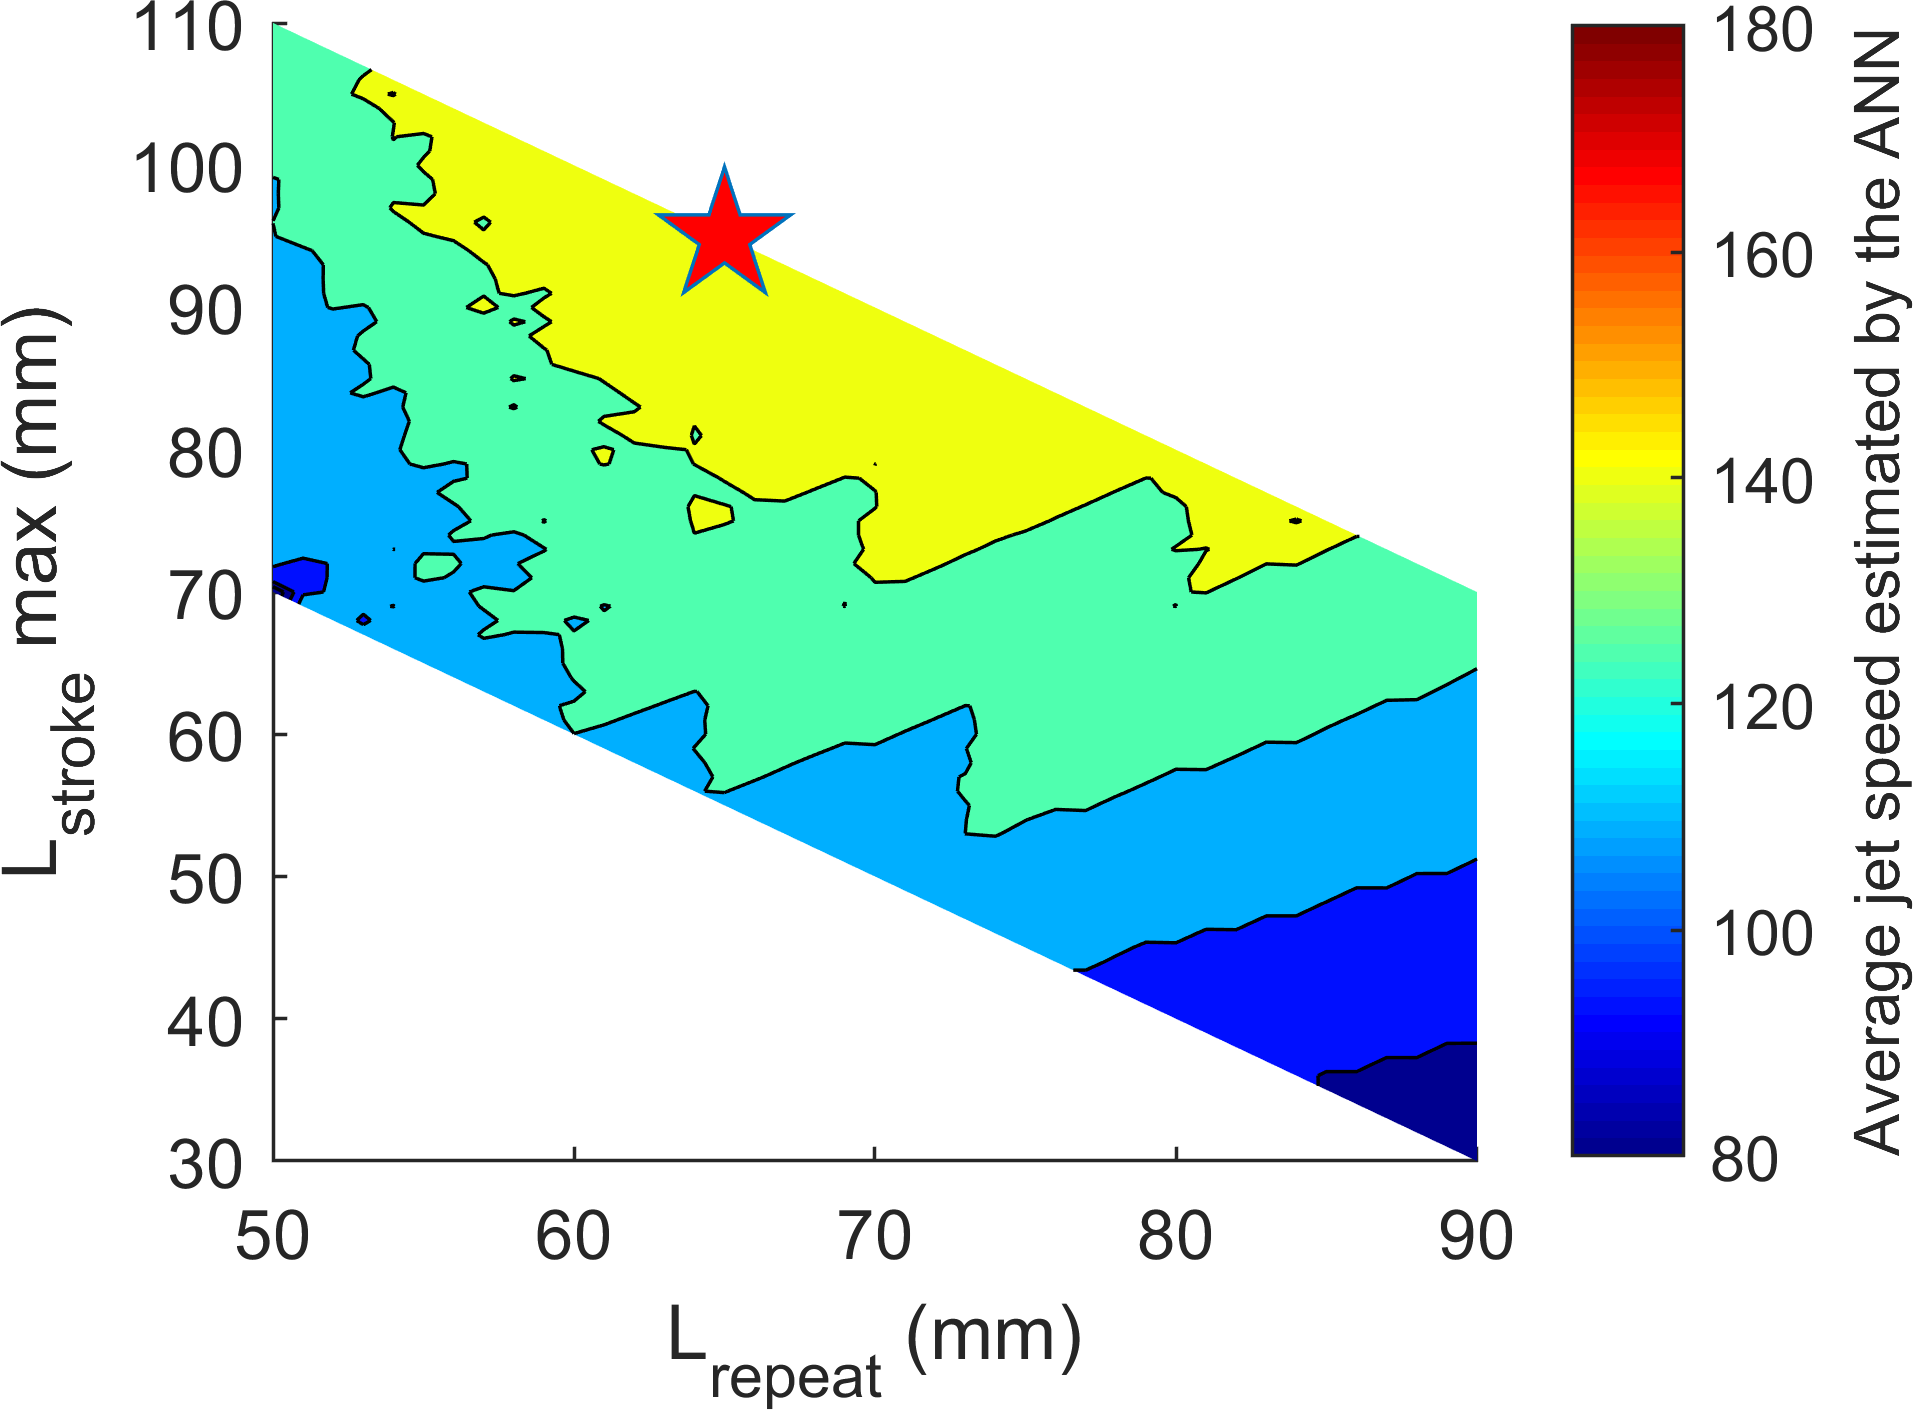
\includegraphics[width=0.45\textwidth]{chap4/images2/325g.png}
                    \label{fig:chapter/rsm/LFSM/optimization/325}
                }
                \qquad
                \subfloat[$M_0=350\,\mathrm{g}$. Global optimum found at $L_{C0}=62\,\mathrm{mm}$, and $L_{S-max}=160\,\mathrm{mm}$.
                ]{
                    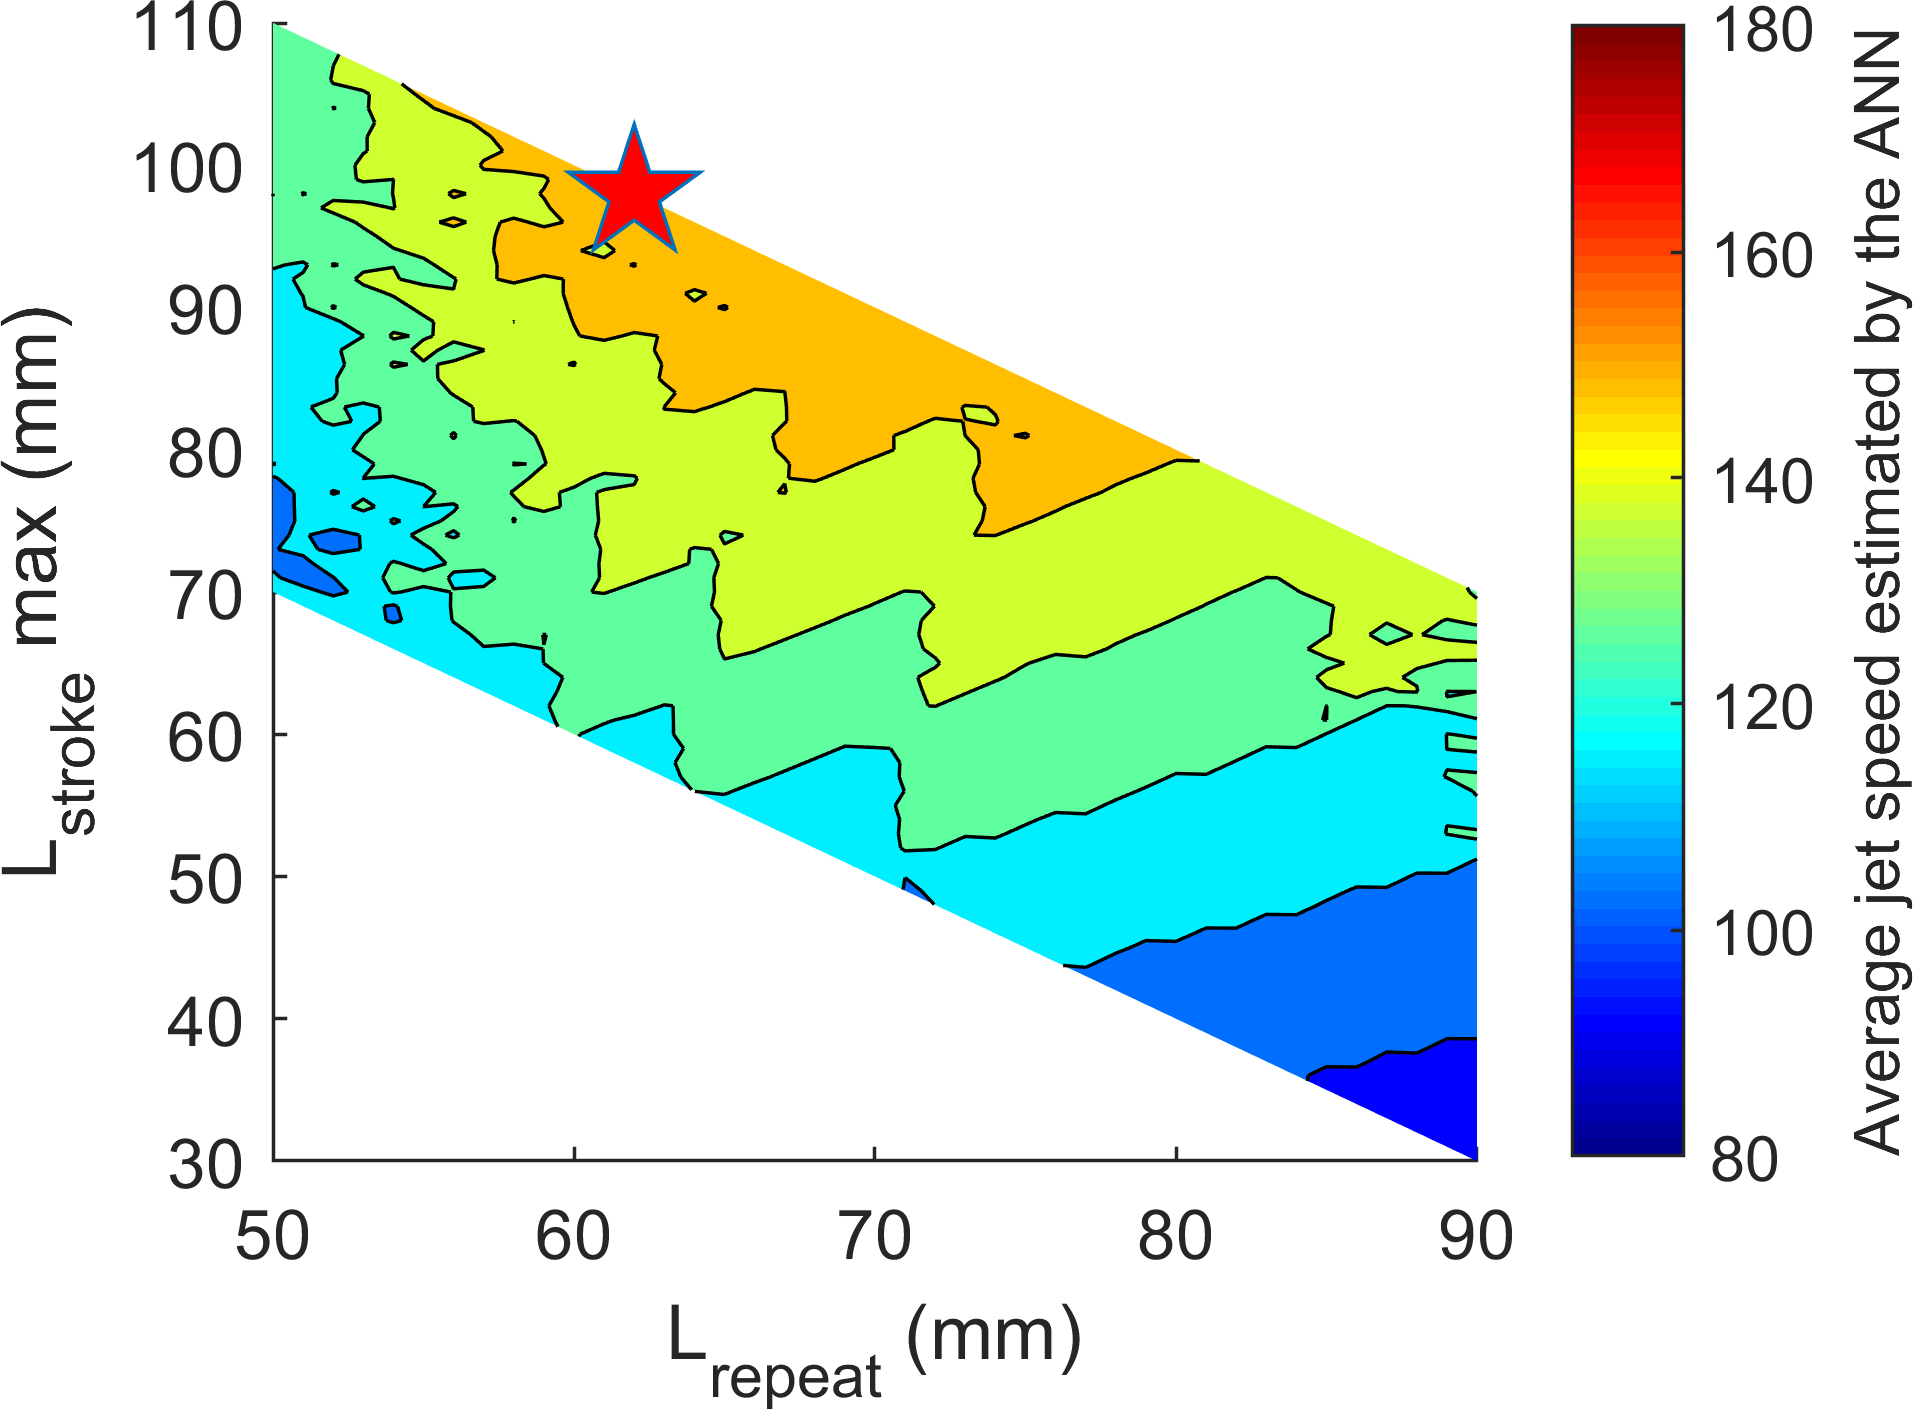
\includegraphics[width=0.45\textwidth]{chap4/images2/350g.png}
                    \label{fig:chapter/rsm/LFSM/optimization/350}
                }
                \\
                \subfloat[$M_0=375\,\mathrm{g}$. Global optimum found at $L_{C0}=70\,\mathrm{mm}$, and $L_{S-max}=160\,\mathrm{mm}$.
                ]{
                    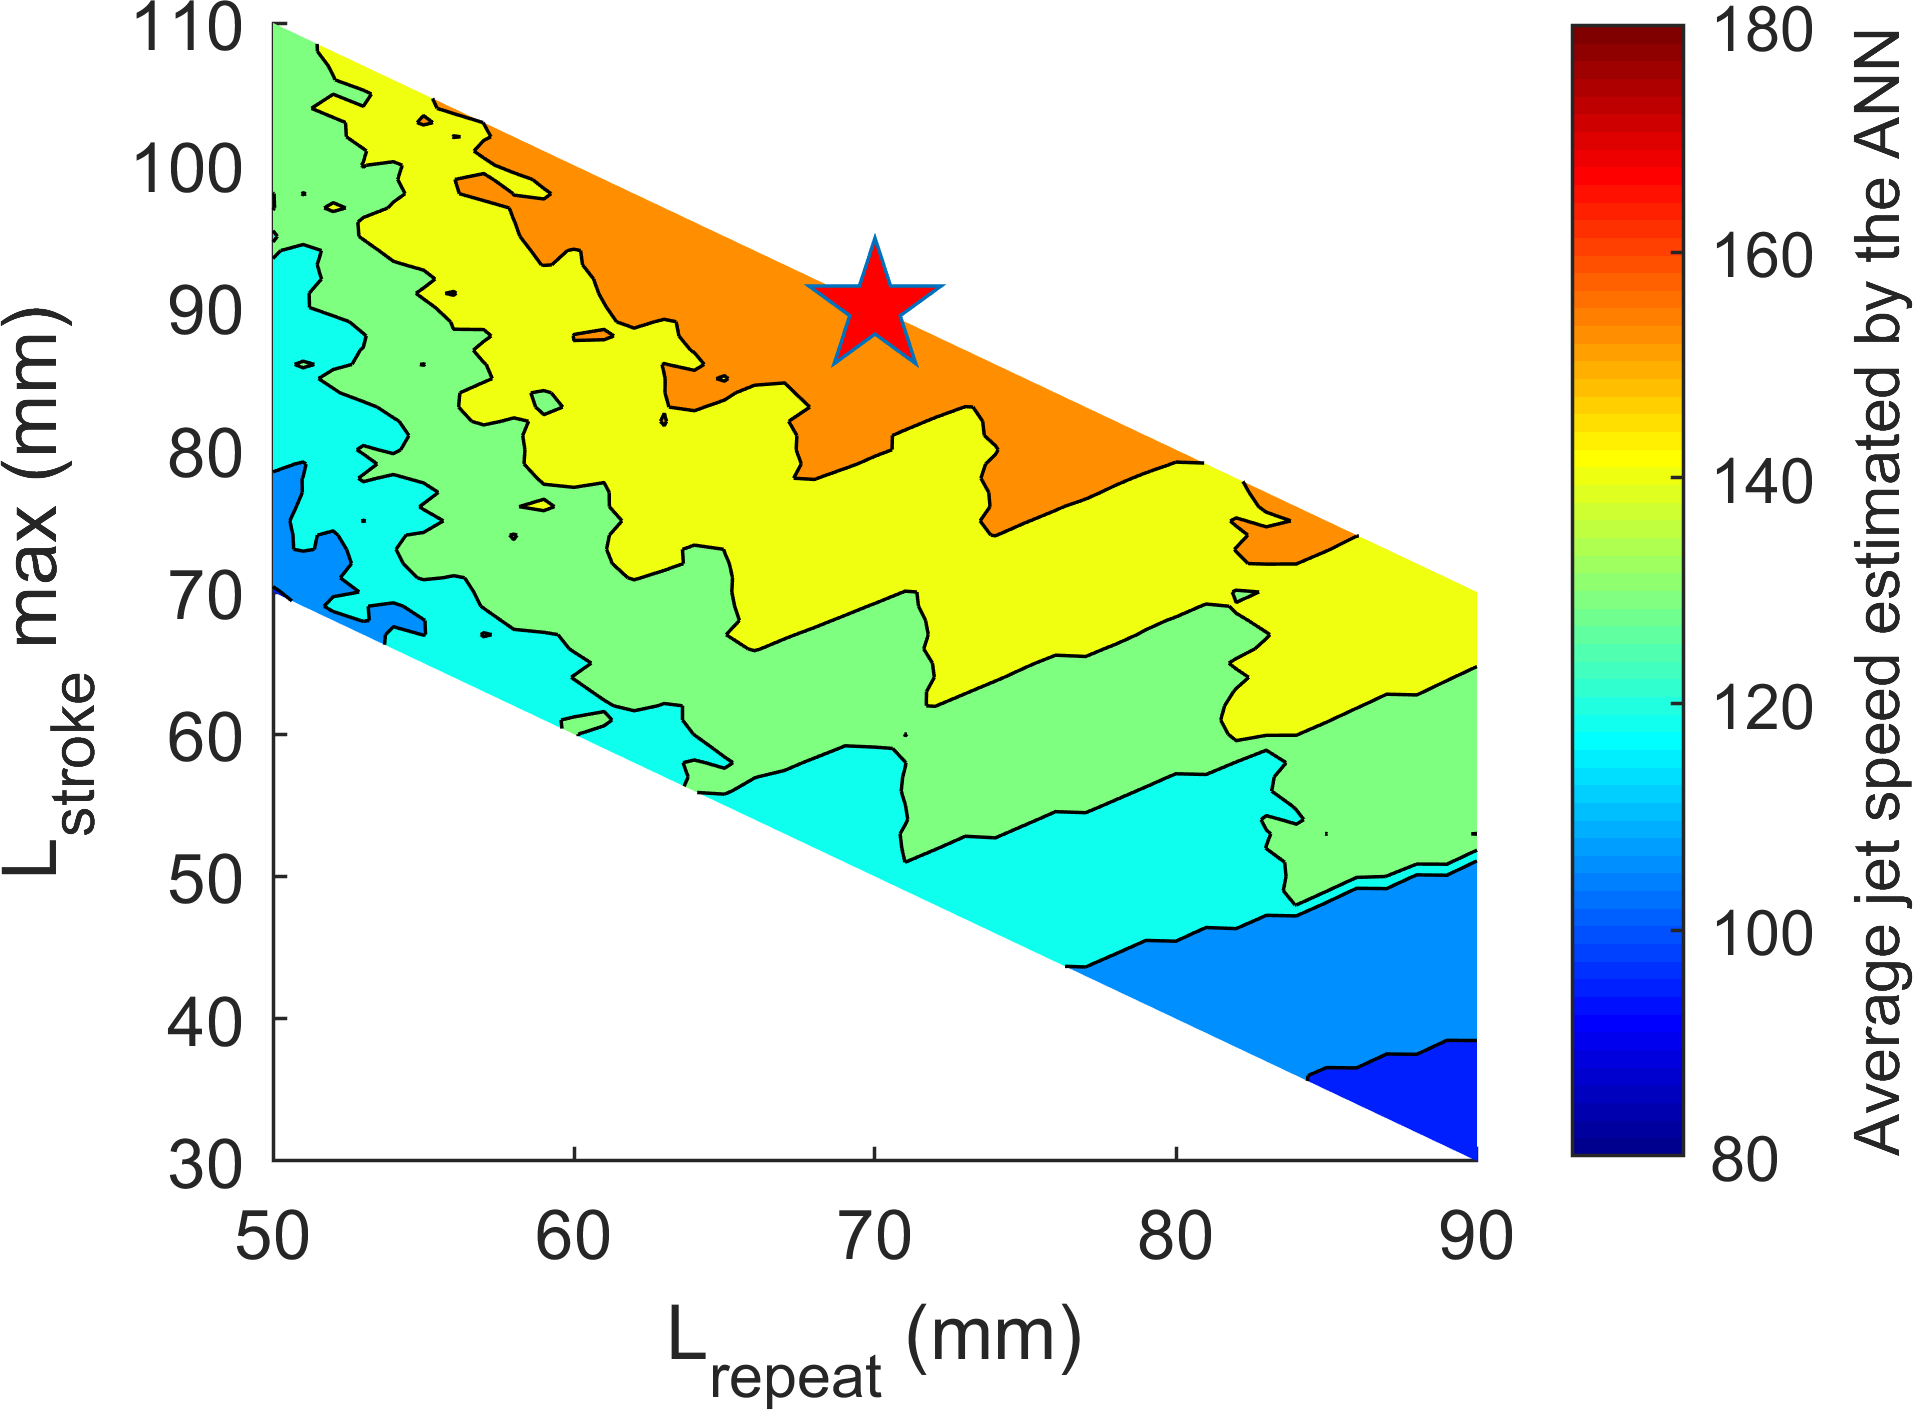
\includegraphics[width=0.45\textwidth]{chap4/images2/375g.png}
                    \label{fig:chapter/rsm/LFSM/optimization/375}
                }
                \qquad
                \subfloat[$M_0=400\,\mathrm{g}$. Global optimum found at $L_{C0}=70\,\mathrm{mm}$, and $L_{S-max}=160\,\mathrm{mm}$.
                ]{
                    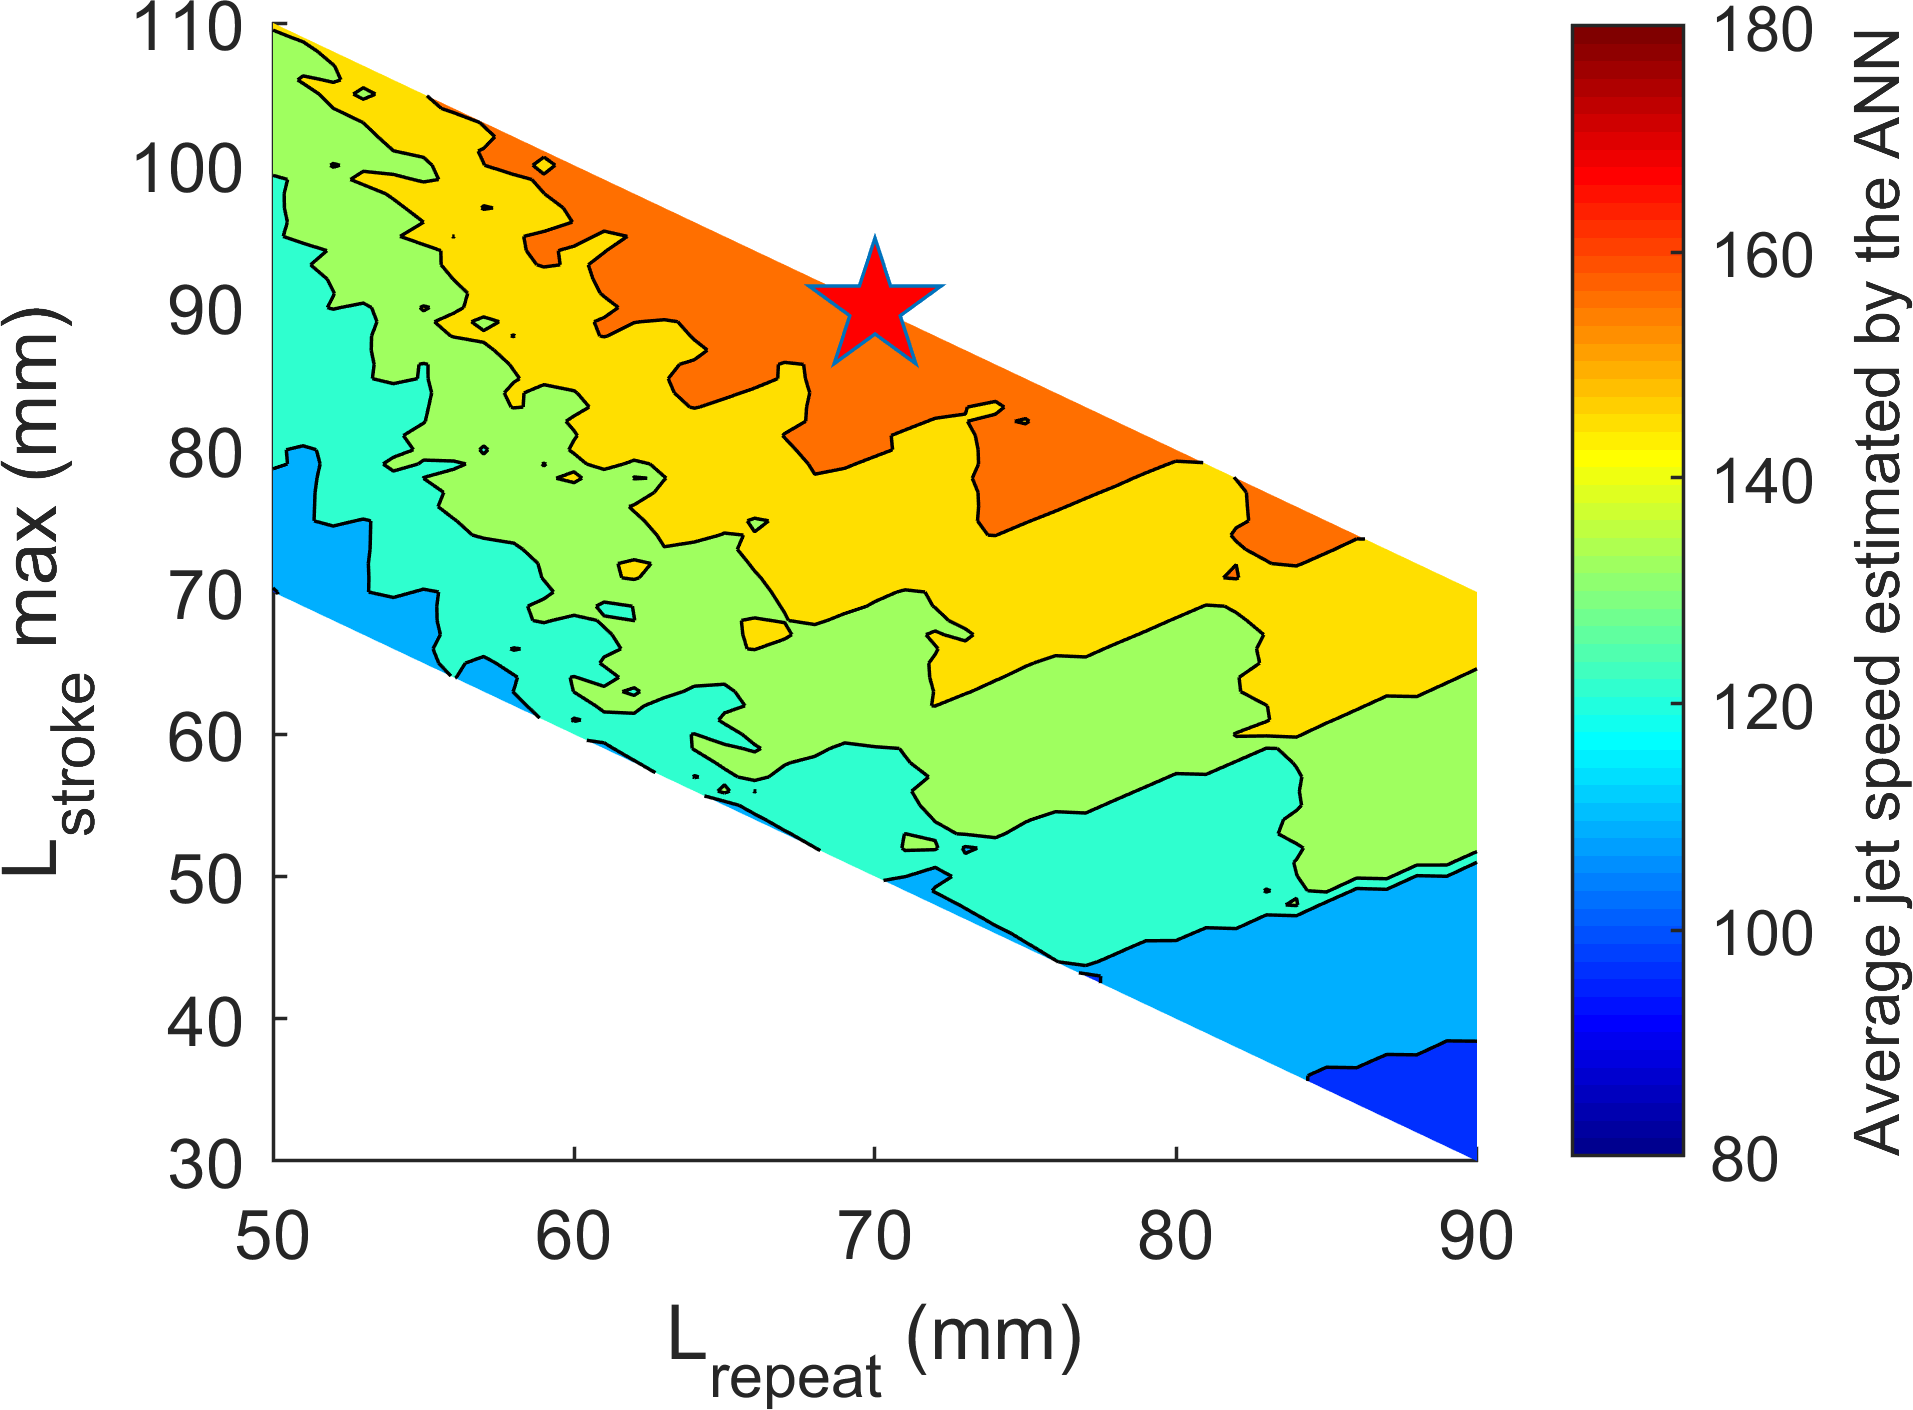
\includegraphics[width=0.45\textwidth]{chap4/images2/400g.png}
                    \label{fig:chapter/rsm/LFSM/optimization/400}
                }
                \\
                \subfloat[$M_0=425\,\mathrm{g}$. Global optimum found at $L_{C0}=70\,\mathrm{mm}$, and $L_{S-max}=160\,\mathrm{mm}$.
                ]{
                    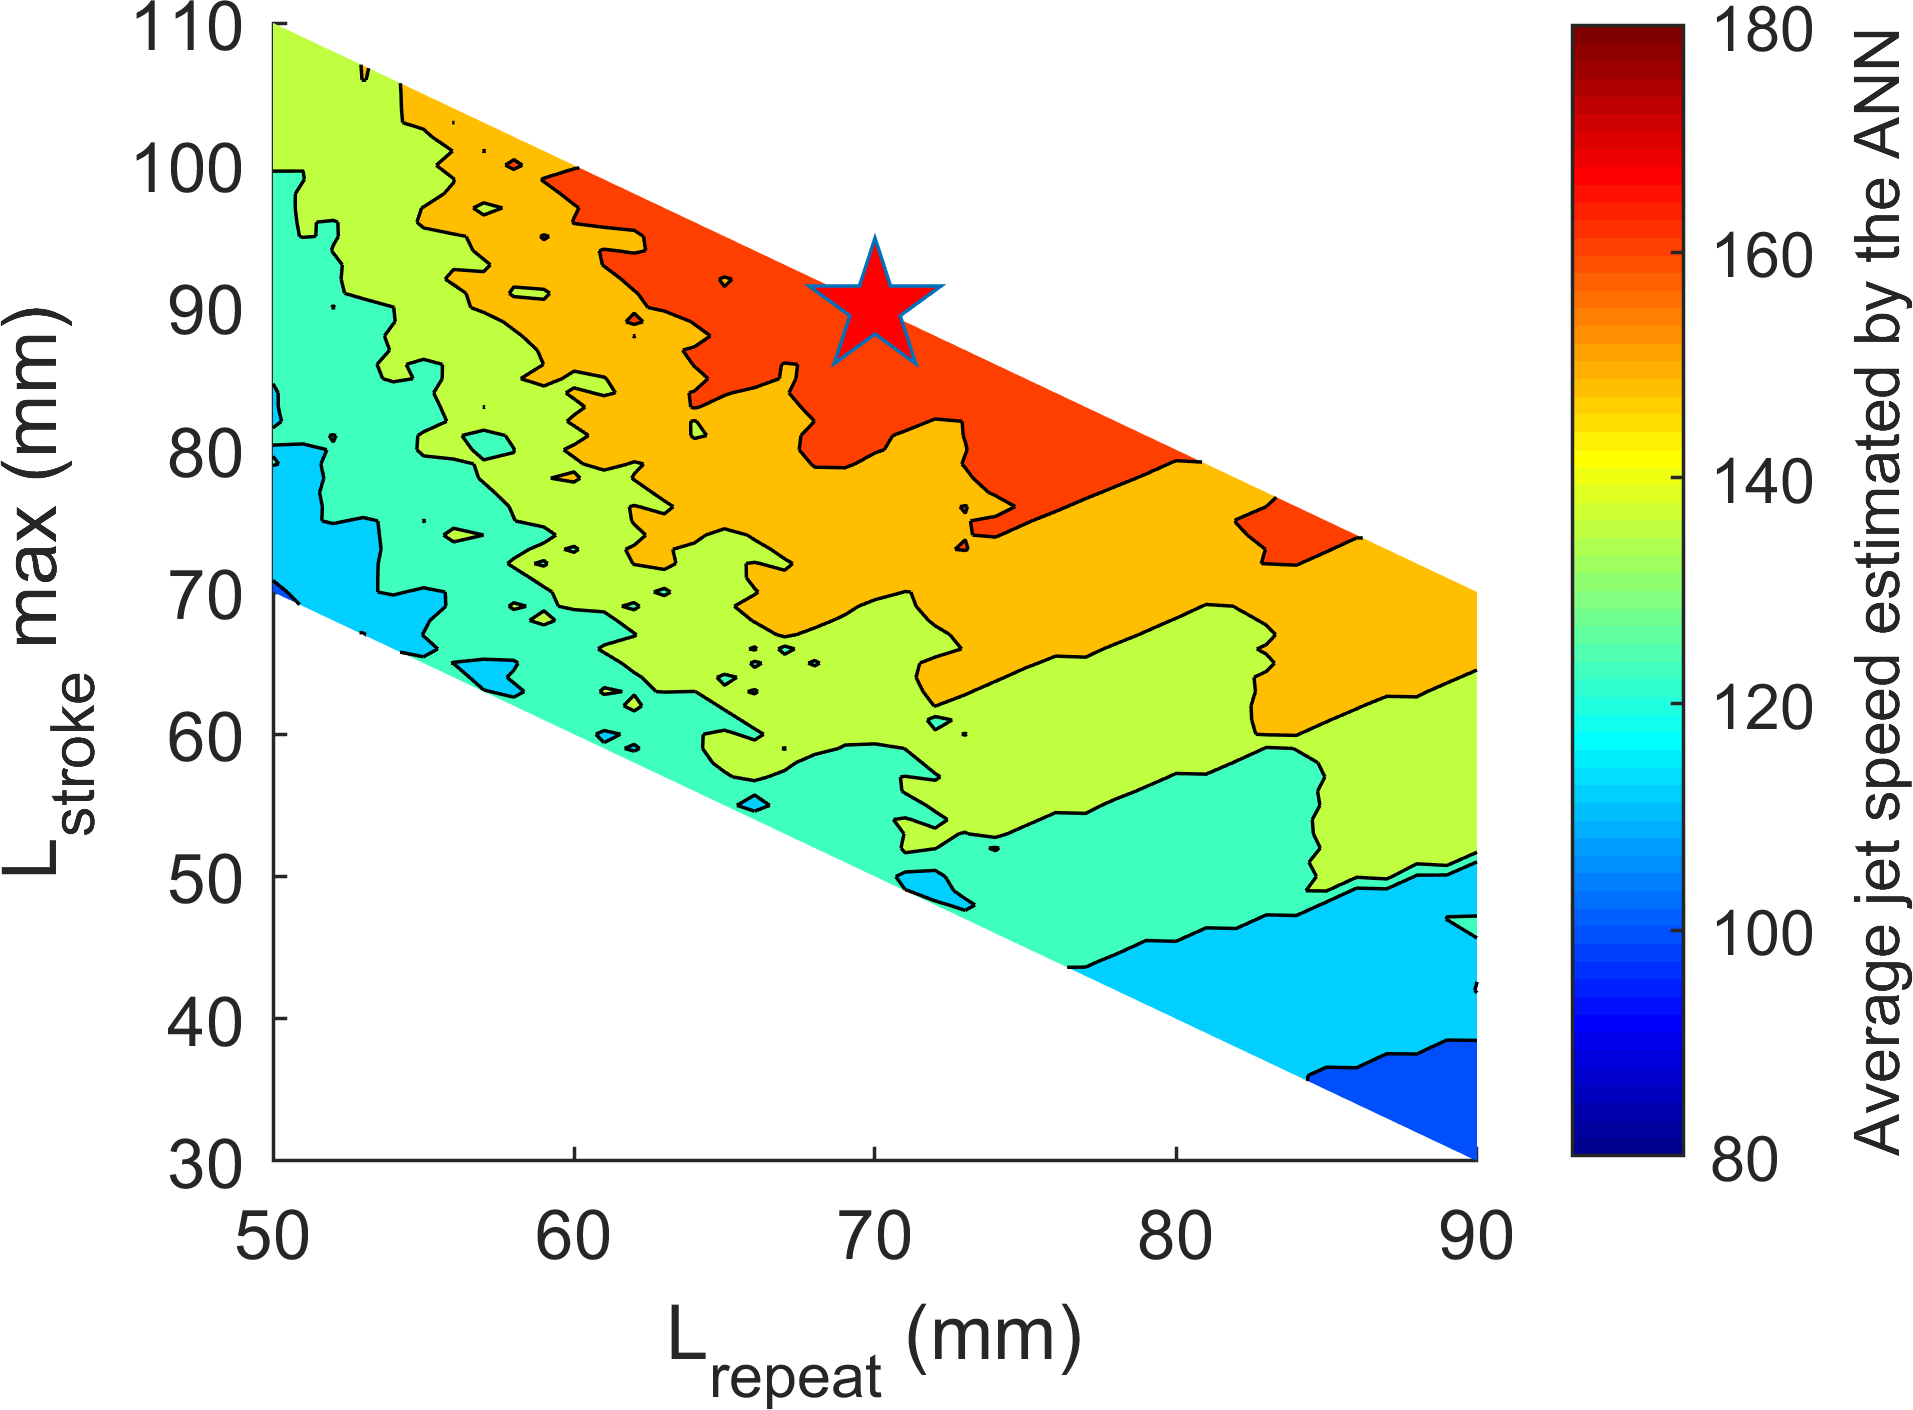
\includegraphics[width=0.45\textwidth]{chap4/images2/425g.png}
                    \label{fig:chapter/rsm/LFSM/optimization/425}
                }
                \\
                \caption{
                    The global optimization plots of $v_{jet}$ for the search space $L_{M0}:120\,\mathrm{mm}\rightarrow 160\,\mathrm{mm} \times L_{C0}:50\,\mathrm{mm}\rightarrow 90\,\mathrm{mm}$ using $P=1500\,\mathrm{W}$, $V=1\,\mathrm{mL}$, $r_{si}=2\,\mathrm{mm}$, $h_G=1.2\,\mathrm{mm}$, $N_C=6$, $M_0=325\,\mathrm{g}$, $\theta = \arctan{1/2}$,  and $M_0$ of: (a) $325\,\mathrm{g}$, (b) $350\,\mathrm{g}$, (c) $375\,\mathrm{g}$, (d) $400\,\mathrm{g}$, and (e) $425\,\mathrm{g}$.
                }   \label{fig:chapter/rsm/LFSM/optimization search space result for differnt mass}
            \end{figure*}
    
    
    % ===================================================================================================
    % === NEW SECTION === NEW SECTION === NEW SECTION === NEW SECTION === NEW SECTION === NEW SECTION ===
    % ===================================================================================================
    \section{Application to LTFM}               \label{Chapter:RSM/LTFM}
    
        
        Conventional longitudinal flux motors like \acs{PMLSM} and \acs{LFSM} requires short repeat lengths for high force density applications because the magnetic circuit travels in-plane with the direction of motion. However, with shortening the pole pitch, the conductor component become increasingly more difficult to manufacture. In \acf{LTFM}, however, the electric circuit is decoupled from the magnetic circuit, and thus the motor can stay manufacturable as the pole pitch shortens. This is because the flux path lies perpendicular to the direction of motion. With this fundamental difference, it is expected that \acs{LTFM} might be able to perform better in short stroke, high thrust applications starting from a near stall condition. 
        
        
        \begin{figure}[!ht]
            \centering
            \subfloat[Schematic for a single phase LTFM]{
                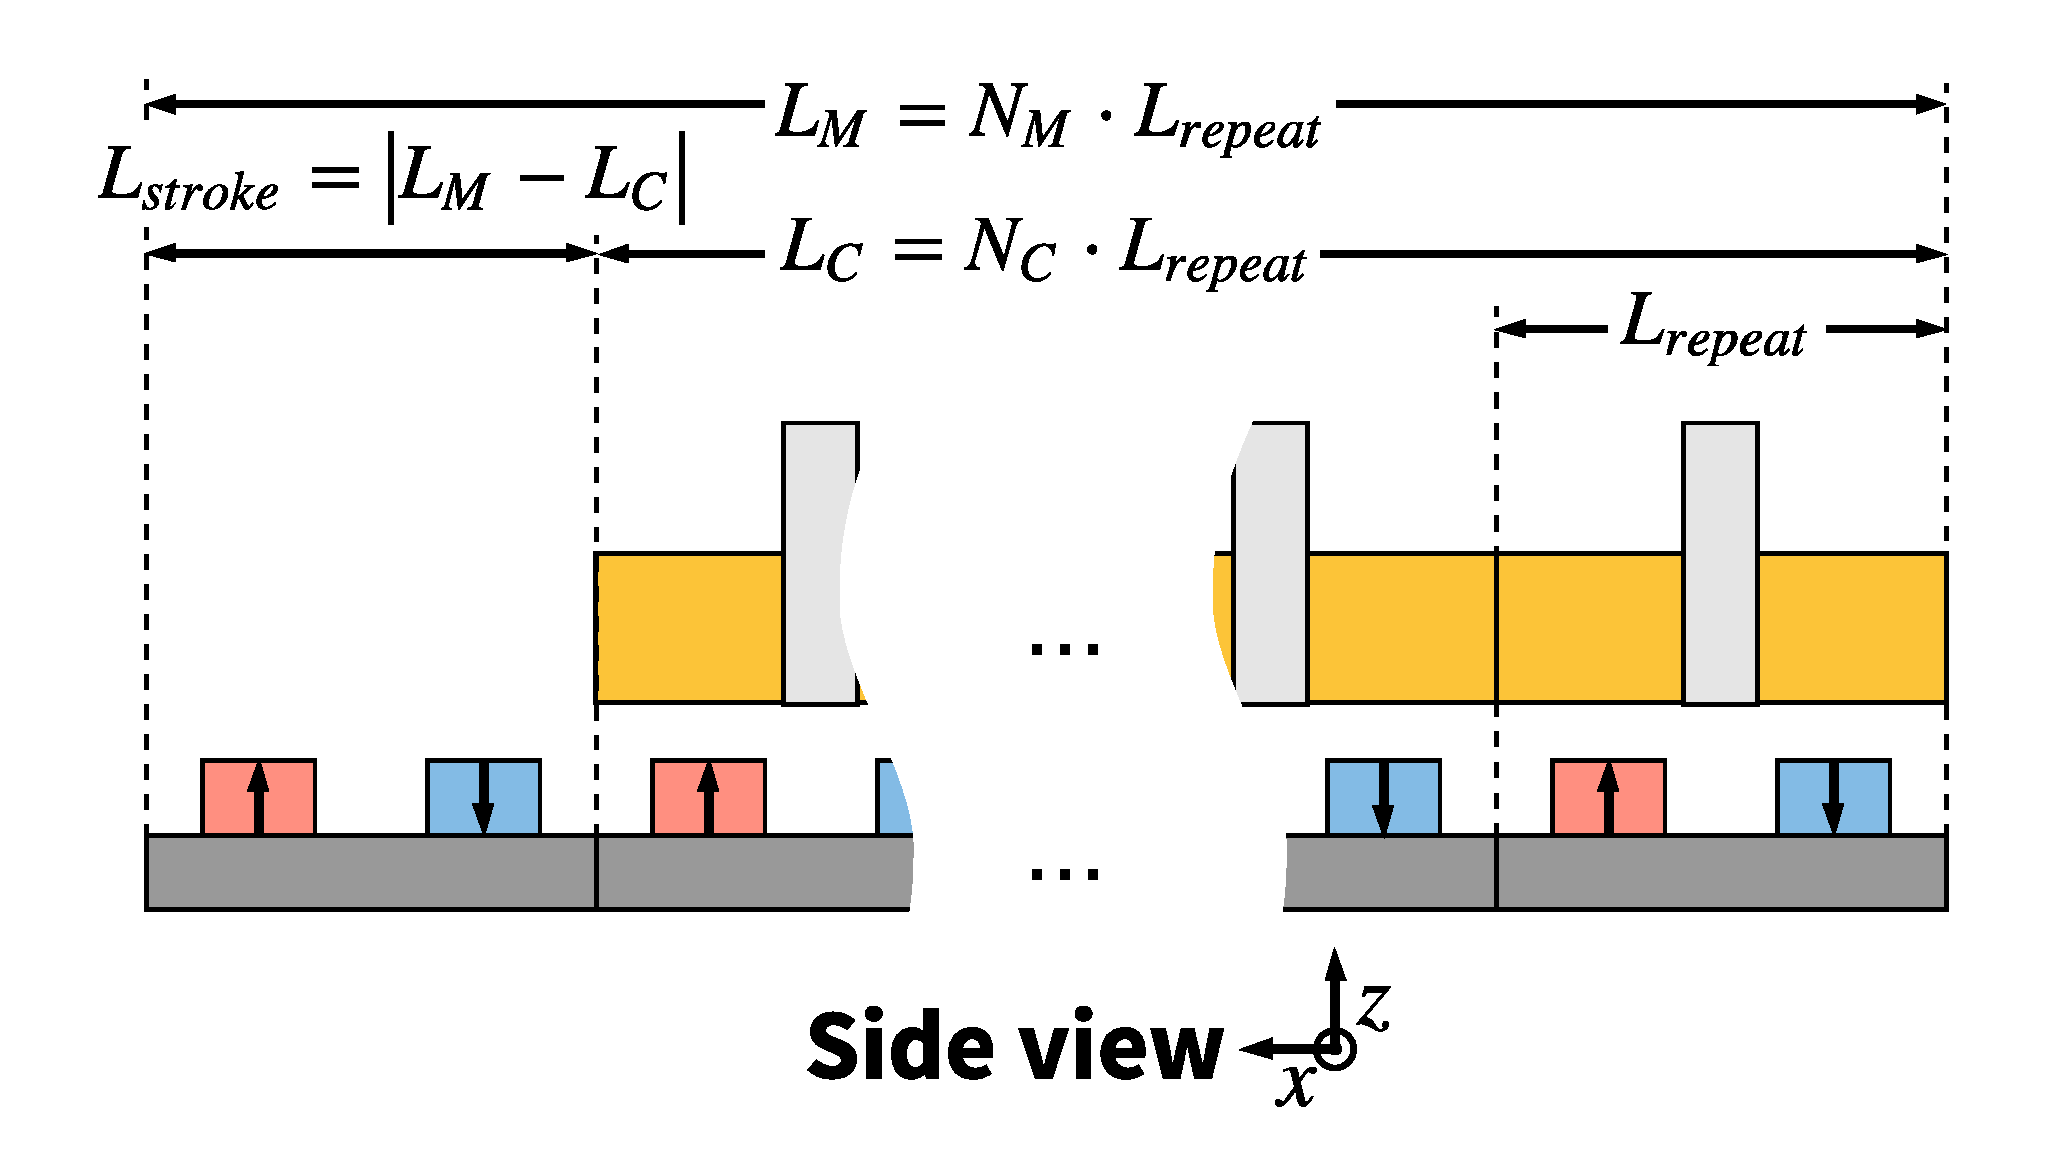
\includegraphics[width=0.75\textwidth]{chap4/images3/TFM_illustration.pdf}
                \label{fig:chapter/rsm/LTFM/illustration}
            }
            \\
            \subfloat[3-phase arrangement for LTFM]{
                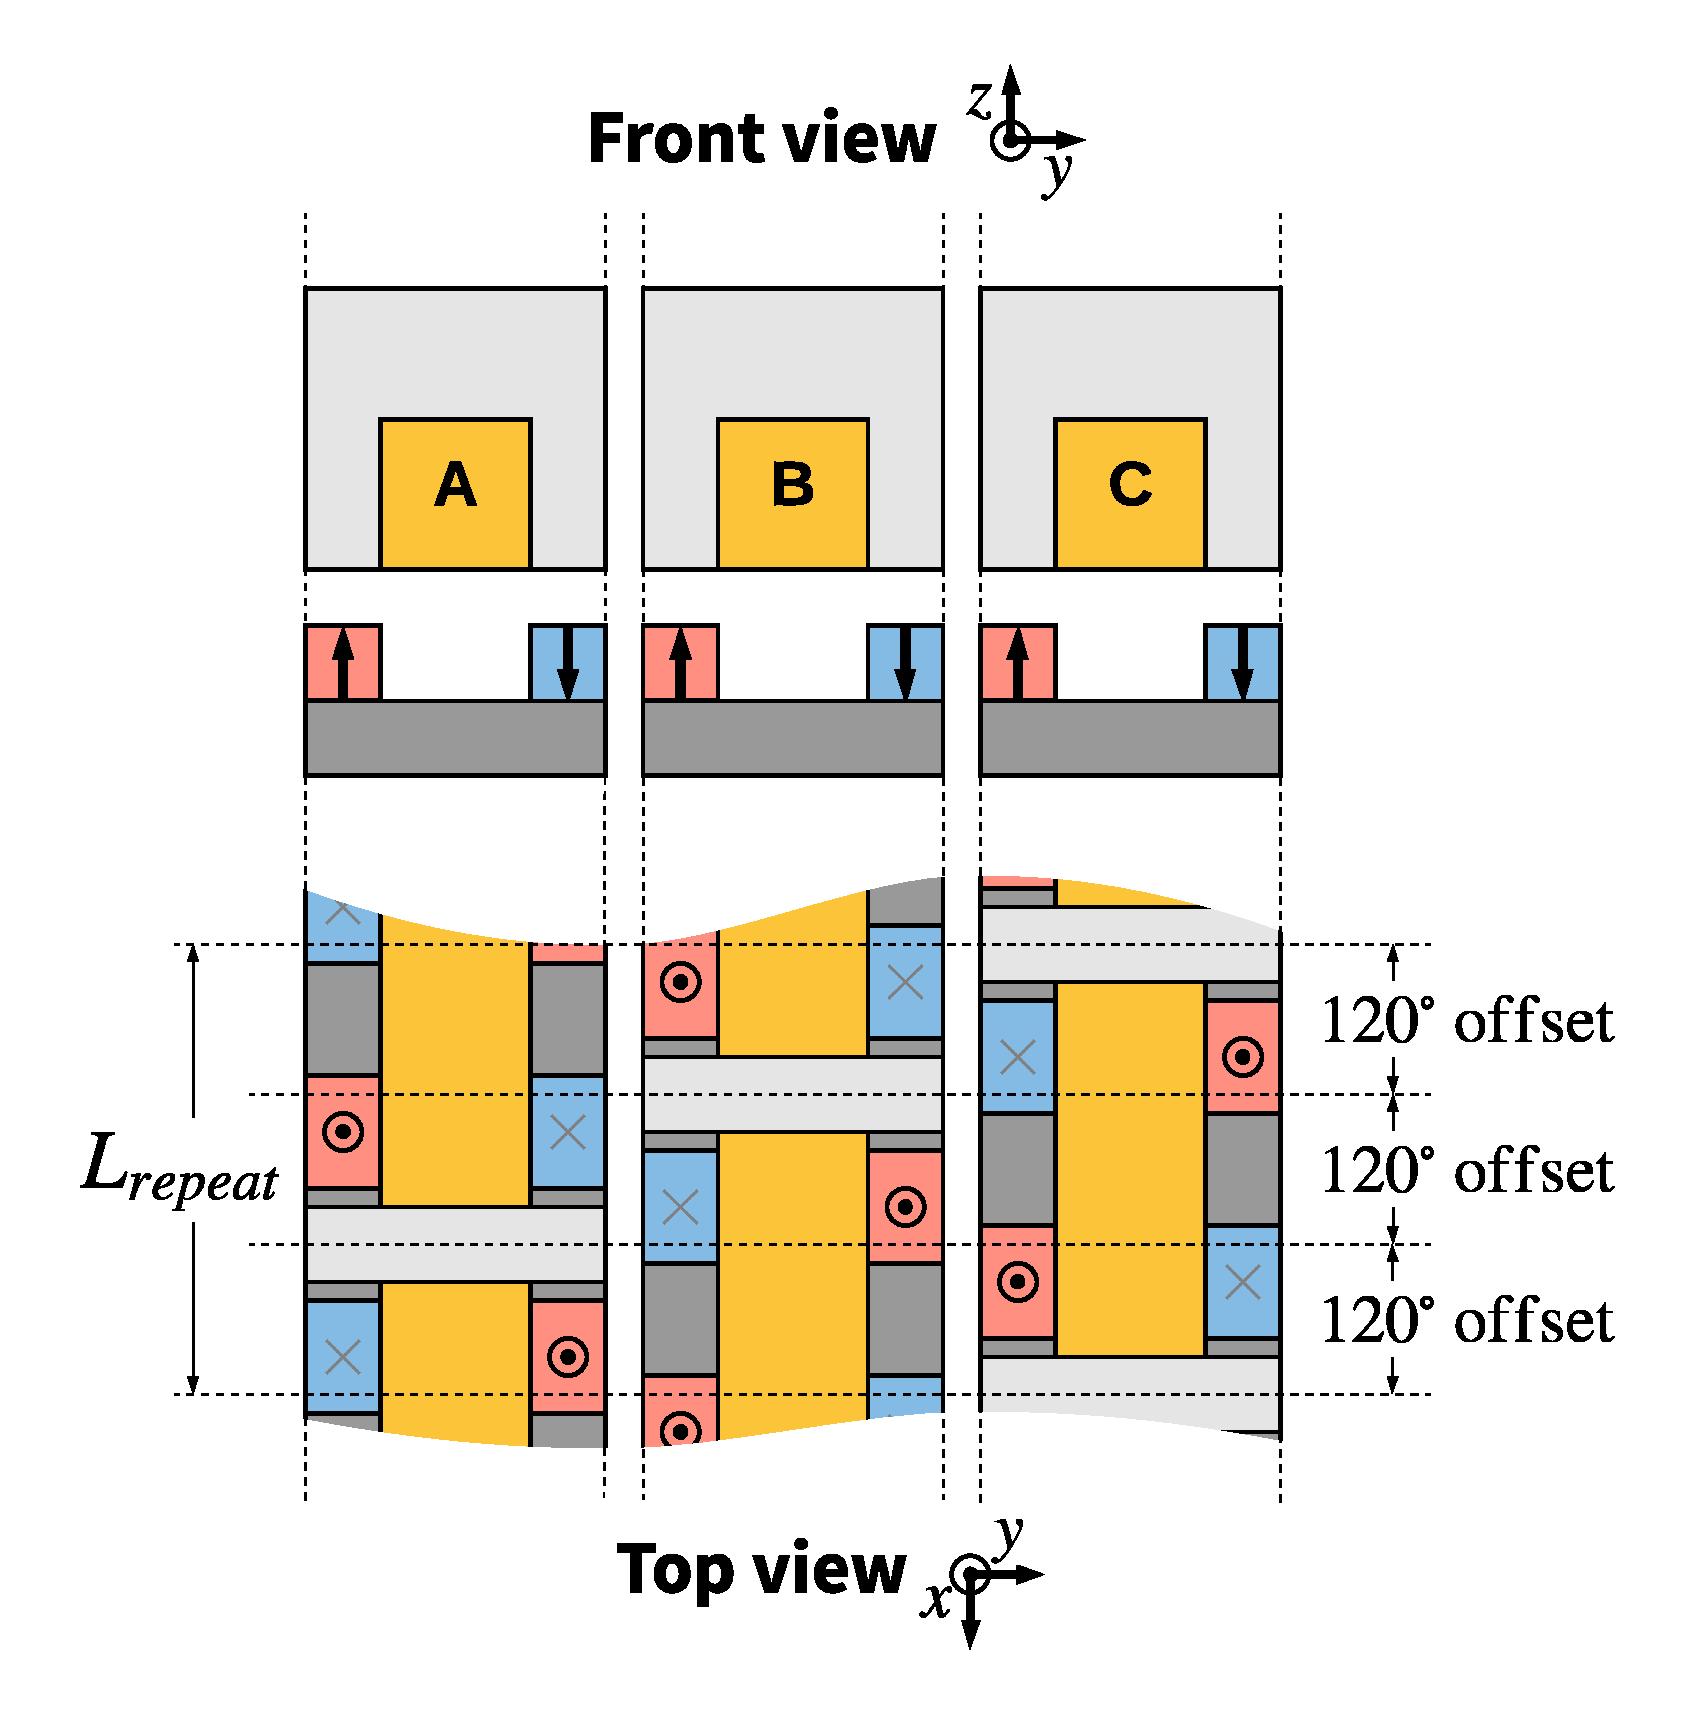
\includegraphics[width=0.5\textwidth]{chap4/images3/TFM_3phase.pdf}
                \label{fig:chapter/rsm/LTFM/3 phase arrangement}
            }
            \caption{Outline of LTFM topology.}
            \label{fig:chapter/rsm/LTFM/different LTFM arrangement}
        \end{figure}

        
        This section aimed to study \acs{LTFM} using the motor design process for high volume \acs{NFJI} applications already applied for \acs{PMLSM} and \acs{LFSM}. The chosen topology was the U-core \acs{LFSM} machine, with surface mounted permanent magnet blocks on a long iron stator as shown in Fig.\,\ref{fig:chapter/rsm/LTFM/illustration}. Unlike the inherent 3-phase winding structure of \acs{PMLSM} and \acs{LFSM}, the body of a \acs{LTFM} contains a single rectangular prism for a single conductor winding. There are positions on the stroke of a single phase \acs{LTFM} in which the conductor winding cannot produce any axial thrust no matter how much current is applied. Therefore, three identical copies of this structure must be placed in parallel, and $120^\circ$ apart to facilitate a relatively constant thrust profile with 3-phase current as shown in Fig.\,\ref{fig:chapter/rsm/LTFM/3 phase arrangement}. 
        
        
        \begin{figure*}[!ht]
            \centering
            \subfloat[Dimension outline for a single repeat unit of the \acs{LTFM}]{
                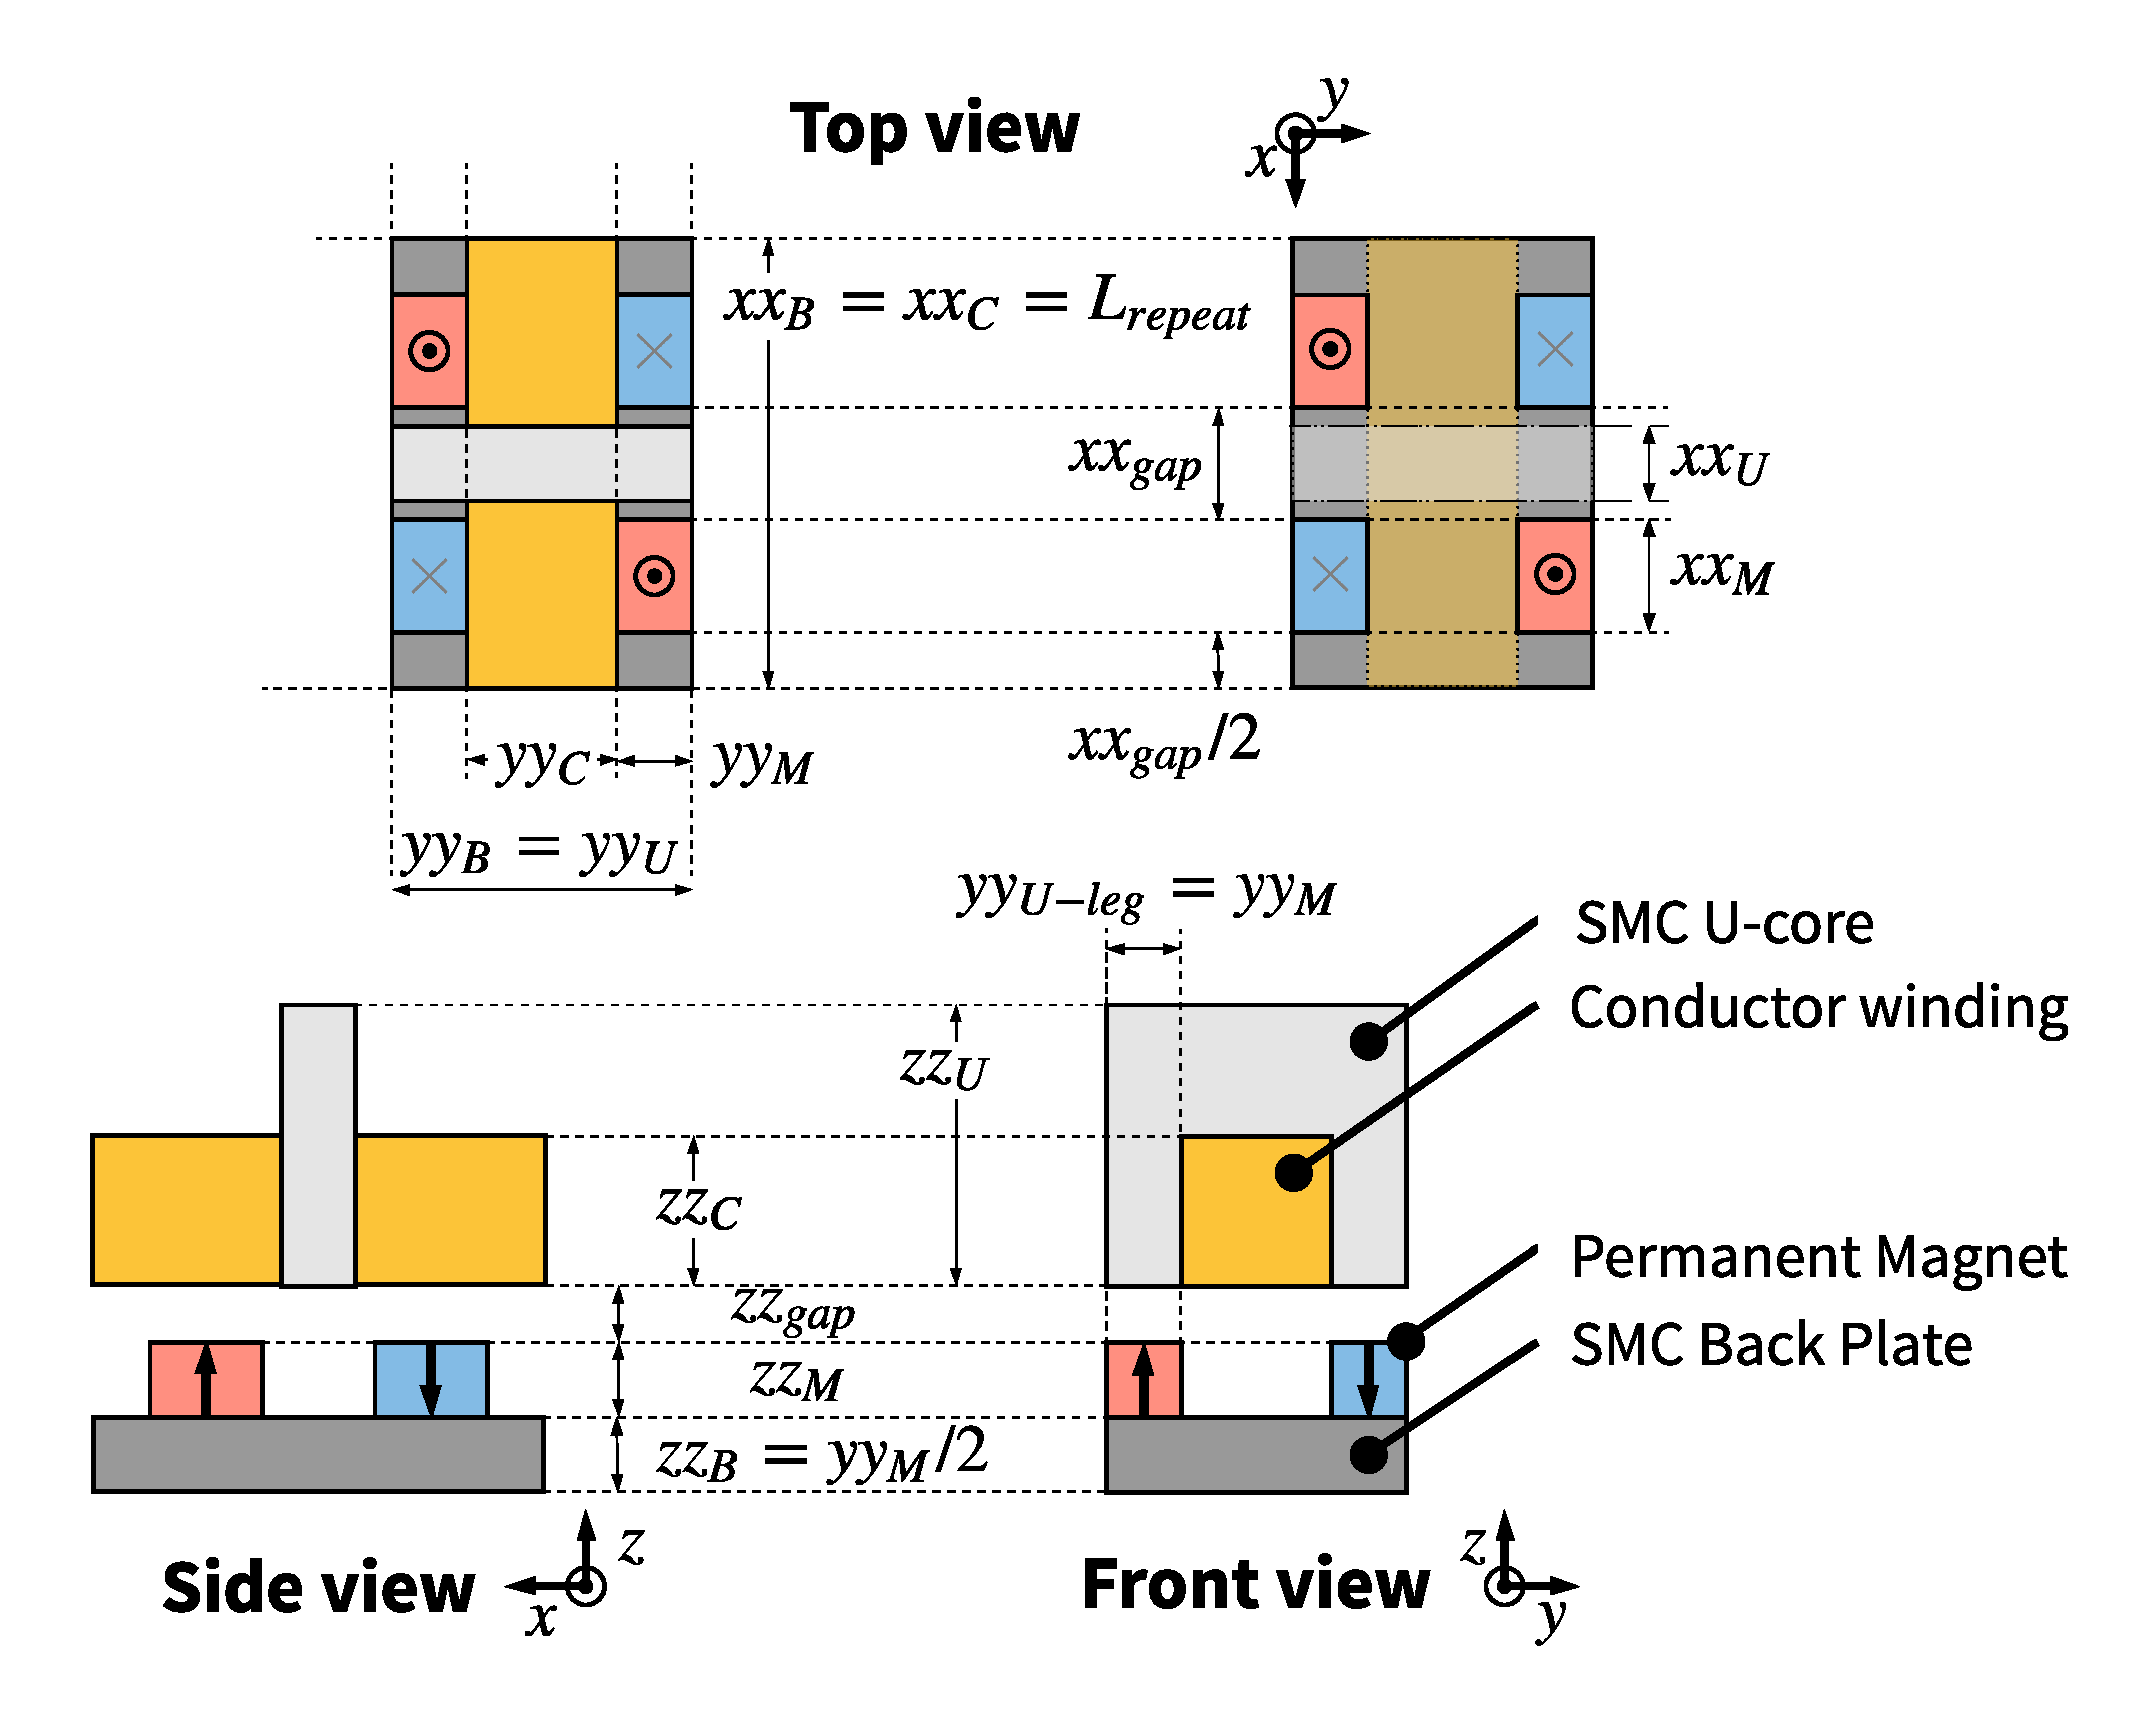
\includegraphics[width=0.95\textwidth]{chap4/images3/TFM_dimensions.pdf}
                \label{fig:chapter/rsm/LTFM/dimensions}
            }
            \\
            \subfloat[The arrangement for using \acs{LTFM} for \acs{NFJI} application]{
                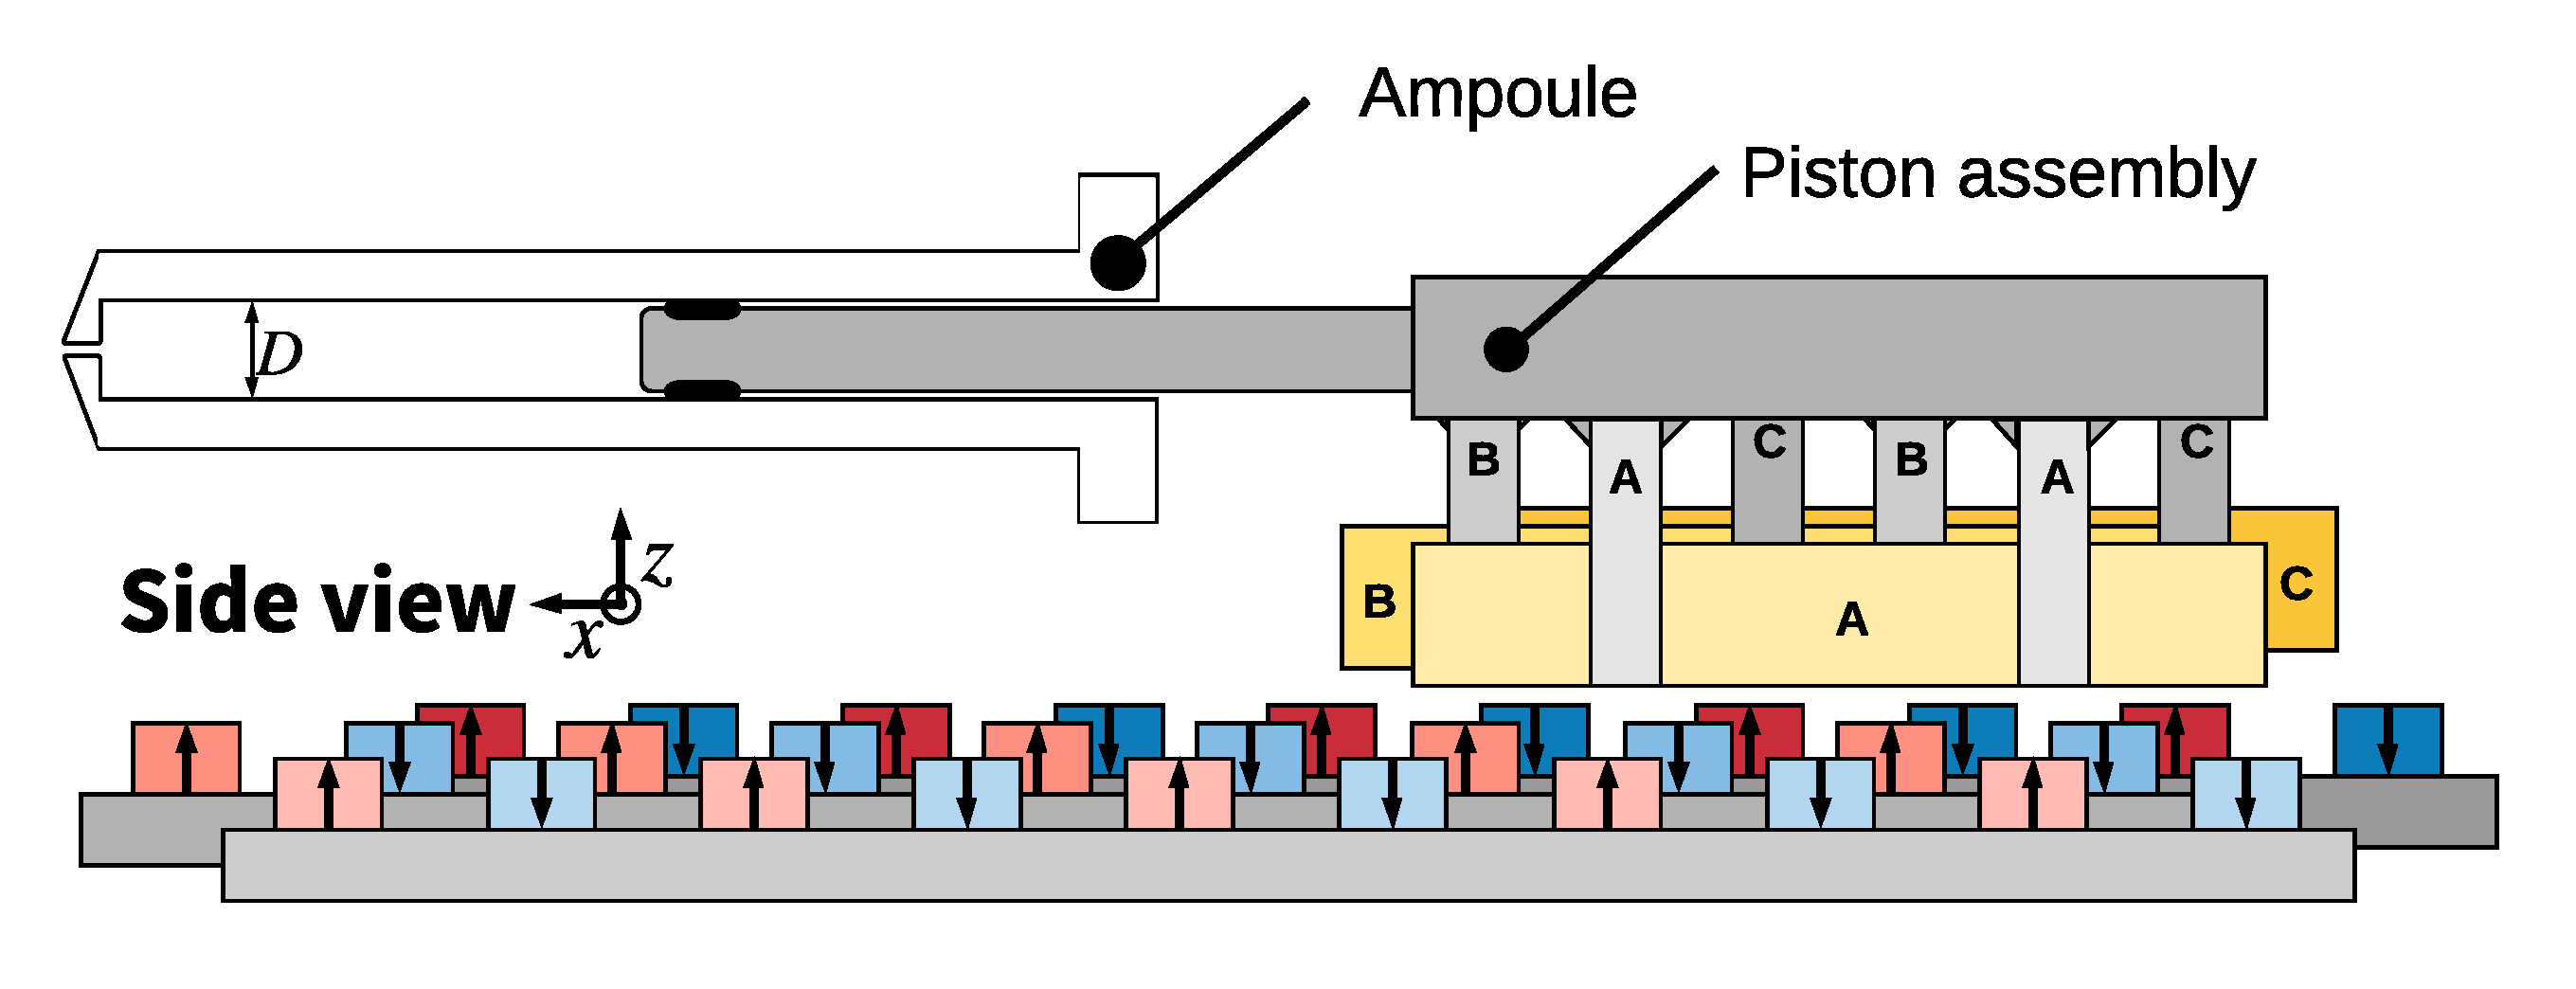
\includegraphics[width=0.85\textwidth]{chap4/images3/TFM_for_NFJI.pdf}
                \label{fig:chapter/rsm/LTFM/used for NFJI}
            }
            \caption{Outline of \acs{LTFM} in \acs{NFJI} application.}
            \label{fig:chapter/rsm/LTFM/3-phase and NFJI}
        \end{figure*}
        
        
         The coil and U-core assembly was chosen to be the mover because this assembly is more likely to be lighter than the magnets and flux conductor plate assembly. Each coil repeating unit consisted of a large conductor winding and U-core made out of prototype \acs{SMC} materials. Each stator repeating unit consisted of four pieces of magnet directed the $y$-axis, and a single long back plate made out of \acs{SMC} material to direct the flux path. Fig.\,\ref{fig:chapter/rsm/LTFM/dimensions} and \ref{fig:chapter/rsm/LTFM/illustration} depict the general parameters of a three-phase transverse flux motor:
        
        \begin{itemize}
            \item The total number of armature repeating unit or pole $N_C$,
            \item The total number of stator and magnets repeating unit or pole $N_M$,
            \item Dimensions related the conductor winding $xx_C$, $yy_C$, and $zz_C$,
            \item Dimensions related to the permanent magnet pieces $xx_M$, $yy_M$, and $zz_M$,
            \item Dimensions related to the U-core made out of \acs{SMC} prototype material $xx_U$, $yy_U$, and $zz_U$,
            \item Dimensions related to the the mover assembly's back plate made out of \acs{SMC} prototype material $xx_B$, $yy_B$, and $zz_B$,
            \item The air gap between the mover and stator assemblies  $zz_{gap}$
            \item The whole of the mover armature length $L_{C}$ for a single phase \acs{LTFM},
            \item The whole track length or equivalent motor length $L_{M}$ for a single phase \acs{LTFM},
            \item Length of an overall repeat unit $L_{repeat}$,
            \item The motor stroke length $L_{stroke}$.
        \end{itemize}
        
        
        \begin{figure*}[!ht]
            \centering
            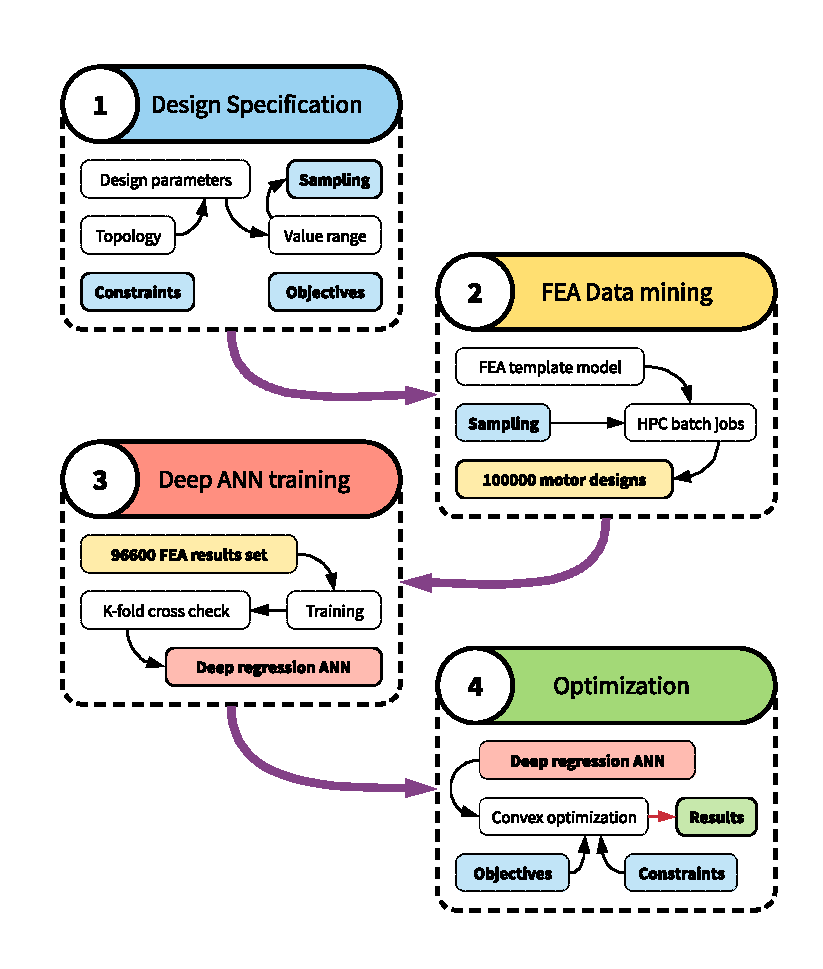
\includegraphics[width=5in]{chap4/images3/TFM_process_summary.pdf}
            \caption{Flowchart of the RSM motor design process adapted for \acs{LTFM}.}
            \label{fig:chapter/rsm/LTFM/design process}
        \end{figure*}
        
        
        The different lengths of the motor are governed by the following set of equations:
        
        
        \begin{equation}
            L_M = N_M L_{repeat}
            \label{eq:chap/rsm/LTFM/L_M}
        \end{equation}
        
        
        \begin{equation}
            L_C = N_C L_{repeat}
            \label{eq:chap/rsm/LTFM/L_C}
        \end{equation}
        
        
        \begin{equation}
            L_{M-3-phase} = \bigg(1+\frac{2}{3} \bigg) N_M L_{repeat} 
            \label{eq:chap/rsm/LTFM/L_M_3phase}
        \end{equation}
        
        
        \begin{equation}
            L_{C-3-phase} = \bigg(1+\frac{2}{3}\bigg) N_C L_{repeat} 
            \label{eq:chap/rsm/LTFM/L_C_3phase}
        \end{equation}
        
        
        \begin{equation}
            L_{stroke} = \big| L_M-L_C \big| = \big| L_{M-3-phase} - L_{C-3-phase} \big|
            \label{eq:chap/rsm/LTFM/L_stroke}
        \end{equation}
        
        
        where $L_{M-3-phase}$ and $L_{C-3-phase}$ are the length of magnet array and armature in a 3-phase \acs{LTFM}.

        
        
        Additional design ratios were established to better capture the parametric representation of the \acs{LTFM}:
        
        
        \begin{equation}
            \alpha=\frac{2\,xx_M}{L_{repeat}}
            \label{eq:chap/rsm/LTFM/alpha}
        \end{equation}
        
        
        \begin{equation}
            \beta=\frac{yy_C}{yy_M}
            \label{eq:chap/rsm/LTFM/beta}
        \end{equation}
        
        
        \begin{equation}
            \gamma=\frac{zz_U}{zz_C}
            \label{eq:chap/rsm/LTFM/gamma}
        \end{equation}
        
        
        For the rigidity of the structure, the coil and the SMC back plate should be made continuous in motors with non-unity pole numbers. For this very reason, the dimensions $xx_B$ and $xx_C$ were assumed to be equal to $L_{repeat}$:
        
        
        \begin{equation}
            xx_B = xx_C = L_{repeat}
            \label{eq:chap/rsm/LTFM/xb is xc is lrepeat}
        \end{equation}
        
        
        To further simply the topology, $xx_M$, and $yy_M$ were set to be equal to $xx_U$, and $y$-dimension for the U-core leg $yy_{U-leg}$, in the same order:
        
        
        \begin{equation}
            xx_M=xx_U
            \label{eq:chap/rsm/LTFM/xm is xu}
        \end{equation}
        
        
        \begin{equation}
            yy_M=yy_{U-leg}
            \label{eq:chap/rsm/LTFM/ym is yuleg}
        \end{equation}
        
        
        The thickness of the \acs{SMC} back plate was also simplified to be half the value of $yy_{M}$:
        
        
        \begin{equation}
            zz_B=\frac{yy_M}{2}
            \label{eq:chap/rsm/LTFM/zb is half of ym}
        \end{equation}
        
        
        The way in which the \acs{LTFM} can be utilized to deliver \acs{NFJI} shots is illustrated in Fig.\,\ref{fig:chapter/rsm/LTFM/used for NFJI}. The process summary of optimizing the \acs{LTFM} topology described above is illustrated in Fig.\,\ref{fig:chapter/rsm/LTFM/design process}.
        

        % -----------------------------------------------------------------------------------
        % --- NEW SUB SECTION --- NEW SUB SECTION --- NEW SUB SECTION --- NEW SUB SECTION --- 
        % -----------------------------------------------------------------------------------
        \subsection{Specifications \& Samplings}    \label{Chapter:RSM/LTFM/spec}
        
            
            This work investigated and optimized the U-core \acs{LTFM} machine with the dimensions presented in Fig.\,\ref{fig:chapter/rsm/LTFM/dimensions} and \ref{fig:chapter/rsm/LTFM/illustration}. With consideration of the dimensions and ratios of the desired motor design, the structural design factors and their ranges are summarized in Table\,\ref{table:chap/rsm/LTFM/design range}. 
            
            
            With consideration of the dimensions and ratios of the optimized motor designs in \cite{Kremers2015}, the structure design factors with their value ranges are summarized table\,\ref{table:chap/rsm/LTFM/design level}. From the full factorial of these design levels, there were $40000$ design cases. On top of that, $60000$ randomly generated design cases within the parameters ranges were added to the collection in order to help the \acs{RSM} fitting process in the next step.
            
            
            \begin{table}[h]
                \renewcommand{\arraystretch}{1.2}
                \caption{Summary of \acs{LTFM} parameters range}
                \label{table:chap/rsm/LTFM/design range}
                \centering
                \begin{tabular}{@{}llr@{}}
                \hline
                \bfseries Parameter & \bfseries Description & \bfseries Values\\
                \hline
                    $\alpha$	    & Ratio of $xx_M$ over half period length $L_{repeat}/2$  &	$0.3-0.9$\\ 
                    $\beta$	        & Ratio of coil width $yy_C$ over $yy_M$	&	$1.0-3.0$\\ 
                    $\gamma$	    & Ratio of $zz_U$ over coil height	$zz_C$	&	$0.3-0.7$\\ 
                    $L_{repeat}$    & Repeat length unit length                 &   $5-30\,\mathrm{mm}$\\
                    $yy_M$	        & Width of magnet pieces 	                &	$2-12\,\mathrm{mm}$\\ 
                    $zz_M$	        & Height of magnet pieces			        &	$2-12\,\mathrm{mm}$\\ 
                    $zz_C$	        & Height of coil winding block 			    &	$3-12\,\mathrm{mm}$\\ 
                    $zz_{gap}$      & Z direction Magnet/Core gap               &	$1.2\,\mathrm{mm}$\\ 
                \hline
                \end{tabular}
            \end{table}
            
            
            \begin{table}
                \renewcommand{\arraystretch}{1.2}
                \caption{Summary of \acs{LTFM} parameters sampling levels}
                \label{table:chap/rsm/LTFM/design level}
                \centering
                    \begin{tabular}{@{}l l l l l l l r@{}}
                    \hline
                    \bfseries Params & \bfseries Level 1 & \bfseries 2 & \bfseries 3 & \bfseries 4 & \bfseries 5 & \bfseries 6 & \bfseries Unit \\
                    \hline
                        $\alpha$	    &   $0.3$   &   $0.5$   &   $0.7$   &   $0.9$ 	&   -       &   -   &n/a\\ 
                        
                        $\beta$	        &   $1$     &   $1.5$   &   $2$ 	&   $2.5$   &  $3.0$    &   -   &n/a\\ 
                        
                        $\gamma$	    &   $0.3$   &   $0.4$   &   $0.5$   &   $0.6$ 	&  $0.7$    &   -   &n/a\\ 
                        
                        $L_{repeat}$	&   $5$     &   $10$    &   $20$    &   $30$ 	&   -       &   -   &$\mathrm{mm}$\\ 
                        
                        $yy_M$	        & 	$2$     &   $3$     &   $6$     &   $9$ 	&	$12$    &   -   &$\mathrm{mm}$\\ 
                        
                        $zz_M$	        & 	$2$     &   $3$     &   $6$     &   $9$ 	&	$12$    &   -   &$\mathrm{mm}$\\ 
                        
                        $zz_C$	        & 	$3$     &   $6$     &   $9$     &   $12$ 	&   -       &   -   &$\mathrm{mm}$\\ 
                        
                    \hline
                    \end{tabular}
            \end{table}
        
        
        % -----------------------------------------------------------------------------------
        % --- NEW SUB SECTION --- NEW SUB SECTION --- NEW SUB SECTION --- NEW SUB SECTION --- 
        % -----------------------------------------------------------------------------------
        \subsection{\acs{FEA} data mining}          \label{Chapter:RSM/LTFM/data mining}
        
        
            Complex physical systems often require \acs{FEA} for accurate numerical calculation at the cost of long computation time, especially when the use of 3-D \acs{FEA} cannot be avoided. Data mining for \acs{LFSM} requires FEA as a means to generate data points for the subsequent regression modelling. 
            
            
            To reduce the complexity of the model, only a single motor phase is simulated at once. We made use of a number of \acs{FEA} techniques to reduce the computation time. As such, the model was enclosed by a 3-D box not much larger than a single motor phase. On the outer surfaces along the direction of motion, a flux parallel boundary condition was applied. In addition to that, the model utilized a periodic boundary condition on surfaces perpendicular to the direction of motion as shown in Fig.\,\ref{fig:chapter/rsm/ltfm/FEA setup}. Hexa-hedral elements were map-meshed, while the free space was freely tetra-hedrally meshed in order to minimize the mesh generation time. The non-linear $B-H$ relationship of the $\mathrm{SGTec\,S700\,5P}$ \acs{SMC} material was fully captured in the \acs{FEA} model. 
            
            
            \begin{figure}[!ht]
                \centering
                \subfloat[Schematic for a FEA setup \acs{LTFM}]{
                    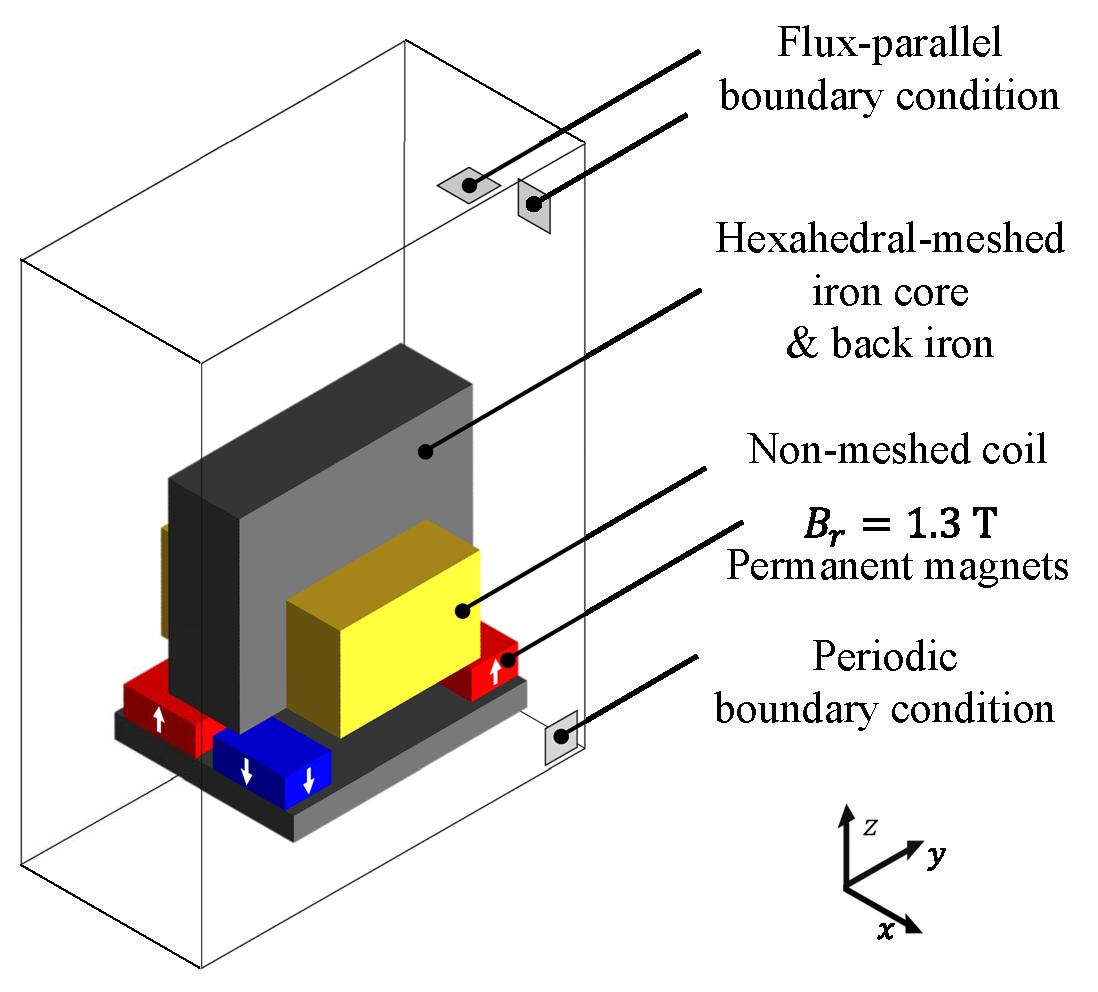
\includegraphics[width=0.6\textwidth]{chap4/images3/FEA_model_v4.pdf}
                    \label{fig:chapter/rsm/ltfm/FEA setup}
                }
                \\
                \subfloat[Mesh view of materials other than air in the FEA of \acs{LTFM}]{
                    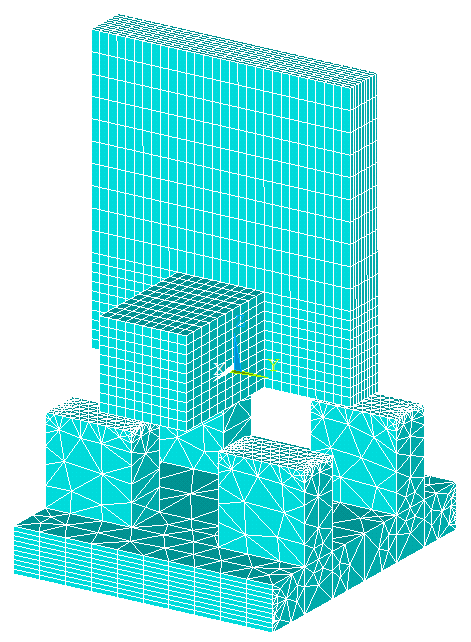
\includegraphics[width=0.32\textwidth]{chap4/images3/TFM_partial_FEA.png}
                    \label{fig:chapter/rsm/ltfm/FEA setup partial}
                }
                \qquad
                \subfloat[Full mesh view in the FEA of \acs{LTFM}]{
                    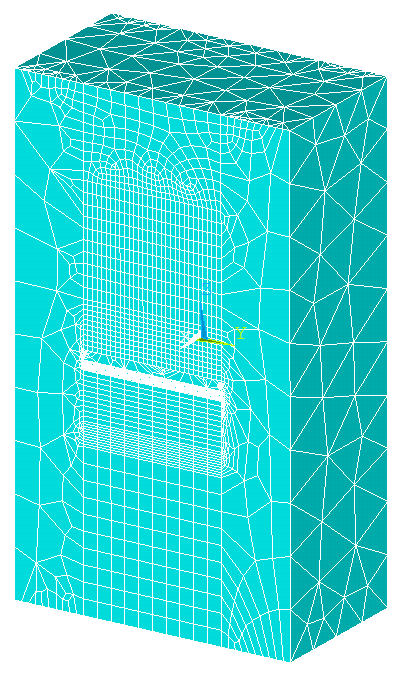
\includegraphics[width=0.25\textwidth]{chap4/images3/TFM_full_FEA.png}
                    \label{fig:chapter/rsm/ltfm/FEA setup full}
                }
                \caption{3-D FEA setup for data minning of \acs{LTFM}}
                \label{fig:chapter/rsm/LTFM/different LTFM FEA setups}
            \end{figure}
            
            
            The \acs{LTFM} consisted of a \acs{SMC} U-Core, a \acs{SMC} back plate, an insulated coil wound around the mover core, and Nd-Fe permanent magnets with $B_r$ of $1.3\,\mathrm{T}$. A fill factor of $60\,\%$ was assumed for the conductor.  The base template for the \acs{FEA} model was constructed in an ANSYS Mechanical APDL $19.2$ script with the intention of allowing for easy modification of the input parameters. The mesh element is $\mathrm{SOLID236}$ which allowed for both electromagnetic hexa-hedral and tetra-hedral meshes where specified.
  
            
            For \acs{LTFM}, the position of the U-core relative to the magnet pieces was very important in maximizing the output thrust for a given input power $P$. The thrust was maximized when the U-core was positioned exactly in the middle of the magnet array along the $x$-axis. With the same logic it was tested to confirm that the thrust was always close to $0\,\mathrm{N}$ when the U-core is aligned with any two magnet pieces in the $z$-axis. This phenomenon explains why there needs to have to be three parallel phases of \acs{LTFM}. This setup guarantees that the mover assembly never gets locked into any particular stroke position.
            
            
            Estimating the motor constant with unit $\mathrm{N/\sqrt{W}}$ for \acs{LTFM} was not used because unlike \acs{PMLSM}, the measurement of motor constant for \acs{LTFM} reaches a plateau much quicker as the current density increases. \acs{LFSM} only needed to work with $1$ power input level, and multiple armature positions because the optimization problem allows for \acsp{LFSM} to have only $1$ armature repeat unit. To recall, in a single armature unit of \acs{LFSM}, there are six wound windings which is enough to facilitate for 3-phase current. Both of these situations did not apply to \acs{LTFM}; therefore, the data mining requires thrust measurement at multiple current density level, and multiple U-core offset positions. There required a conversion process to convert the thrust prediction given current density to a thrust prediction given the electrical power.
            
            Taking one end of the motor repeat unit as position $0$, and the other end as position $1$, the U-core is naturally positioned at $0.5$ as depicted in previous Fig.\,\ref{fig:chapter/rsm/LTFM/different LTFM arrangement} and \ref{fig:chapter/rsm/LTFM/dimensions}. If the U-core moves in the extreme range of $0-0.25$ or $0.75-1$, the U-core risks exceeding the periodic boundary of the \acs{FEA} model. Besides, in these extreme ranges, presuming the current direction persists, the thrust profile is the exact opposite when compared to the thrust profile of the position range $0.25-0.75$. Further more, as discussed previously, the thrusts produced at position $0.25$ and $0.75$ were always near $0\,\mathrm{N}$, much in disregard to any current density input. 
            
            
            To account for both high current sensitivity and position sensitivity of \acsp{LTFM}, each of the $100000$ \acs{FEA} jobs measured the thrust for the position list $[0.333,0.416,0.5,0.583,0.666]$ relative to the repeat length $L_{repeat}$. In total there were $500000$ input files. In each of the input files, the \acs{FEA} job repeated the simulation with a the same mesh for the current density list $[0,2,4,8,16,32,64,128,256]\times\mathrm{A/mm^2}$. 
            
            
            The $500000$ input files were executed in the high performance computing infrastructure owned by the New Zealand eScience Infrastructure (NeSI). Each job took six minutes on a two-core Intel CPU with $3\,\mathrm{GB}$ of RAM. Given that the HPC facility allows for any user to execute $1000$ jobs at once, all jobs were completed after $50$ hours. All verbose outputs of jobs were collected to double check for errors and warnings, totalling $750\,\mathrm{GB}$ of raw data. For each unique single phase \acs{LTFM} designs, the measured thrust at all five positions was then compiled to estimate the average thrust of the 3-phase motor at $[0,1,2,4,8,16,32,64,128]\times\mathrm{A/mm^2}$.
            
            
            After a double-checking the process, there were a total of $96600$ valid 3-phase motor designs recorded in CSV format. The resultant success rate for the data mining process was $96.6\,\%$, high than that of \acs{LFSM}.
            
            
        % -----------------------------------------------------------------------------------
        % --- NEW SUB SECTION --- NEW SUB SECTION --- NEW SUB SECTION --- NEW SUB SECTION --- 
        % -----------------------------------------------------------------------------------
        \subsection{Deep regression ANN training}   \label{Chapter:RSM/LTFM/ANN training}
        
            
            The data set provided both the continuous input variables (structural design factors), and the continuous output variable (thrust characteristics at a current density). Similar to \acs{LFSM}, fitting an \acs{RSM} model for \acs{LTFM} is a supervised and regression type of machine learning problem. With comparatively less data points per input variable, training the \acs{ANN} for \acs{LTFM} was more rigorous than training the models for \acs{PMLSM} and \acs{LFSM}. The \acs{ANN} model was implemented in Keras and Tensorflow machine learning frameworks:
            
            
            \begin{itemize}
                \item The eight structural parameters were regarded as the Input Layer: $\alpha$, $\beta$, $\gamma$, $L_{repeat}$, $yy_M$, $zz_M$, and $zz_C$, 
                \item The nine average thrust values at different current density levels for the 3-phase motor designs were regarded as the Output Layer: $\overline{F_{J=0\,\mathrm{A/mm^2}}}$, $\overline{F_{J=2\,\mathrm{A/mm^2}}}$, $\overline{F_{J=2\,\mathrm{A/mm^2}}}$, $\overline{F_{J=4\,\mathrm{A/mm^2}}}$, $\overline{F_{J=8\,\mathrm{A/mm^2}}}$, $\overline{F_{J=16\,\mathrm{A/mm^2}}}$, $\overline{F_{J=32\,\mathrm{A/mm^2}}}$, $\overline{F_{J=64\,\mathrm{A/mm^2}}}$, and $\overline{F_{J=128\,\mathrm{A/mm^2}}}$
                \item The Nesterov-Adam optimizer was used for \acs{ANN} training, instead of the Adam optimizer in previous \acs{ANN} fitting jobs,
                \item There were ten hidden layers in the \acs{ANN}: $512-512-512-512-512-512-512-1024-1024-1024$ of densely connected nodes,
                \item The rectified linear unit (ReLU) activation function was used
for the input and hidden layers,
                \item The linear activation function was used for the output layer,
                \item $\mathrm{L2}$ regularization terms value of $0.02$ were added to the last three hidden layers to prevent over-fitting at the cost of reaching the training and validation errors convergence more slowly,
                \item The error to optimize for is \acs{MAPE},
                \item The training and validation split chosen at random for each of the three models are: $70\%-30\%$, $75\%-25\%$, and $80\%-20\%$,
                \item The final \acs{ANN} model is ensembled from the average of three models above.
            \end{itemize}
            
            
            After $500$ training iterations, the model was shown to have a \acf{MAPE} of under $3.68\,\%$. Fig.\,\ref{fig:chapter/rsm/LTFM/training result} shows that the training and validation errors were similar, which means the deep regression model is not over-fitted to the training data set.
            
            
            \begin{figure*}[h]
                \centering
                \subfloat[$70\%-30\%$ split model
                ]{
                    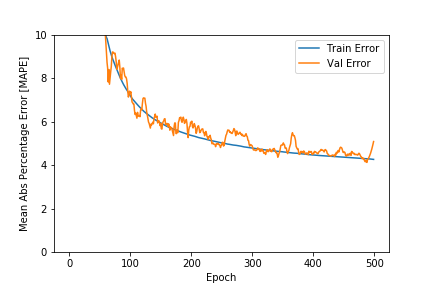
\includegraphics[width=0.48\textwidth,trim={0.5cm 0 0 0.5cm},clip]
                    {chap4/images3/MAPE_6_70_30_MAPE_plot.png}
                    \label{fig:chapter/rsm/LTFM/training result/MAPE_70_30}
                }
                \subfloat[$75\%-25\%$ split model
                ]{
                    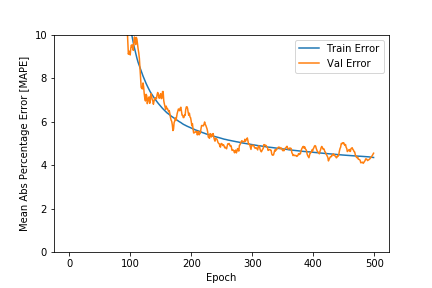
\includegraphics[width=0.48\textwidth,trim={0.5cm 0 0 0.5cm},clip]
                    {chap4/images3/MAPE_6_75_25_MAPE_plot.png}
                    \label{fig:chapter/rsm/LTFM/training result/MAPE_75_25}
                }
                \\
                \subfloat[$80\%-20\%$ split model
                ]{
                    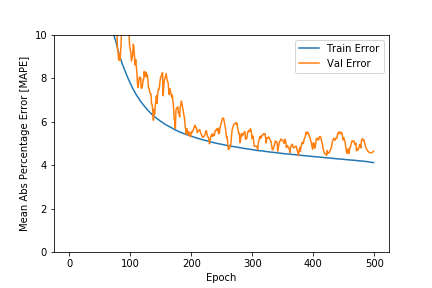
\includegraphics[width=0.5\textwidth,trim={0.5cm 0 0 0.5cm},clip]
                    {chap4/images3/MAPE_6_80_20_MAPE_plot.png}
                    \label{fig:chapter/rsm/LTFM/training result/MAPE_80_20}
                }
                \caption{
                    Error produced by the deep learning ANN model to represent \acsp{LTFM} vs. iterations for the training data (blue) and validation data (orange). The \acs{MAPE} is plotted for the training process of (a) $70\%-30\%$, (b) $75\%-25\%$, and (c) $80\%-20\%$ models, respectively.
                }   \label{fig:chapter/rsm/LTFM/training result}
            \end{figure*}


            It should be noted that the \acs{ANN} structures for \acs{PMLSM}, \acs{LFSM} and \acs{LTFM} are tailored to suit each type of motors. The \acsp{ANN} internal structure, the Input Layer, the Output Layer, regularization terms are unique. 
        
        
        % -----------------------------------------------------------------------------------
        % --- NEW SUB SECTION --- NEW SUB SECTION --- NEW SUB SECTION --- NEW SUB SECTION --- 
        % -----------------------------------------------------------------------------------
        \subsection{Optimization}                   \label{Chapter:RSM/LTFM/Optimization}
        
        
            \subsubsection{Outer optimization}         \label{Chapter:RSM/LTFM/Optimization/Outer}
    
            
                Similar to the optimization problem of \acs{LFSM} for \acs{NFJI} applications, the optimization problem statement needed to be appropriately adjusted to \acs{LTFM} unique characteristics while remaining comparable to the optimization problem of \acs{PMLSM} for \acs{NFJI} applications. With multiple armature phases allowed, the optimization formulation for \acs{LTFM} here was especially similar to which of \acs{PMLSM}:
                
                
                \begin{equation}
                    \begin{array}{rll}
                        \textbf{minimize}       & \small{objective\,\,function}     & f(\textbf{x})=\frac{1}{v_{jet}} \\
                        \textbf{subjected to}   & \small{equality\,\,constraint}    & h_1(\textbf{x})=M - M_0= 0\\
                                                &\quad \small{where}                &\quad  M_0\in\left[325,350,375,400,425\right]\,\mathrm{g}\\
                                                &                                   & h_2(\textbf{x})=P - 1500\,\mathrm{W}=0\\
                                                &                                   & h_3(\textbf{x})=L_{C} - L_{C0} = 0\\
                                                &\quad \small{where}                &\quad  L_{C0}\in\left[50,51,...,90\right]\,\mathrm{mm}\\
                                                &                                   & h_4(\textbf{x})=V - 1\,\mathrm{mL} = 0\\
                                                & \small{inequality\,\,constraint}  & g_1(\textbf{x})=L_{M-3-phase}-L_{M-3-phase-0} \leqslant 0\\
                                                &\quad \small{where}                &\quad L_{M-3-phase-0} \in \left[120,121,...,160\right]\,\mathrm{mm} \\
                                                & \small{other\,\,constraint}       & N_C, N_M \in 	\mathbb{N} \\
                    \end{array}
                    \label{eq:outer optimization for LTMFs}
                \end{equation}
                
                
                \begin{itemize}
                    \item   Limited the search to motors with a total length $L_{M-3-phase-0}$ in between $120\,\mathrm{mm}$ and $160\,\mathrm{mm}$,
                    \item   Divided the maximum allowed magnet array length $L_{M-3-phase-0}$ for all 3 phases into 41 equally spaced values: $[120, 121, 122, ..., 160]\,\mathrm{mm}$ 
                    \item   Divided the coil length $L_{C0}$ of a single phase ranges into 41 equally spaced lists:  $[50, 51, 52, ..., 90]\,\mathrm{mm}$ 
                    \item   Created a $\mathrm{2D}$ search zone for each combination of maximum motor length $L_{M0}$ which includes all three phases and the coil mover length $L_{C}$ of a single phase, totalling $1681$ points,
                    \item   Ran $1681$ inner optimization searches with the Matlab constrained convex non-linear optimization function $fmincon()$. Details of the inner optimization will be explained below,
                    \item   Plotted and identified a motor design that could produce the highest average jet speed $v$ at the given mass constraint $M$.
                \end{itemize}
                
                

                
                
                Given each combination of $L_{C0}$ and $L_{M-3-phase-0}$, a set of $N_C$ and $L_{repeat}$ within the range specified in Table\,\ref{table:chap/rsm/LTFM/design range} can be determined:
                
                
                \begin{equation}
                    N_C \in \Bigg[\bigg\lceil {\frac{L_{C0}}{\mathrm{Max}(L_{repeat)}}} \bigg\rceil:\bigg\lfloor{\frac{L_{C0}}{\mathrm{Min}(L_{repeat})}}\bigg\rfloor\Bigg] 
                    \label{eq:chap/rsm/LTFM/list of N_C}
                \end{equation}
            
                
                \begin{equation}
                    L_{repeat} \in \frac{L_{C0}}{[N_C]}
                    \label{eq:chap/rsm/LTFM/list of L_repeat}
                \end{equation}
                
                
                The caution here was to make sure the numbers of coil-phase $N_C$ and magnet-phase $N_M$ are simultaneously a natural number, as well as maximizing the total length of motor $L_{M-3-phase-0}$ allowed. When choosing a particular $N_C$ and accompanying $L_C$ from the value sets worked out above, the stroke lengths $L_{stroke}$ and $N_M$ satisfy the following:
    
                
                \begin{equation}
                    L_{stroke} = \Bigg\lfloor \bigg(L_{M-3-phase-0}-\frac{2}{3} L_{repeat}\bigg) \frac{ N_C}{L_C} \Bigg\rfloor \frac{L_C}{N_C}-L_C
                    \label{eq:chap/rsm/LTFM/L_stroke_2}
                \end{equation}
                
                
                \begin{equation}
                    N_M = \frac{L_{M-3-phase-0}-\frac{2}{3} L_{repeat}}{L_{repeat}}
                    \label{eq:chap/rsm/LTFM/N_M}
                \end{equation}


            \subsubsection{Inner optimization}         \label{Chapter:RSM/LTFM/Optimization/Inner}
            
                \begin{figure*}[h]
                  \centering
                  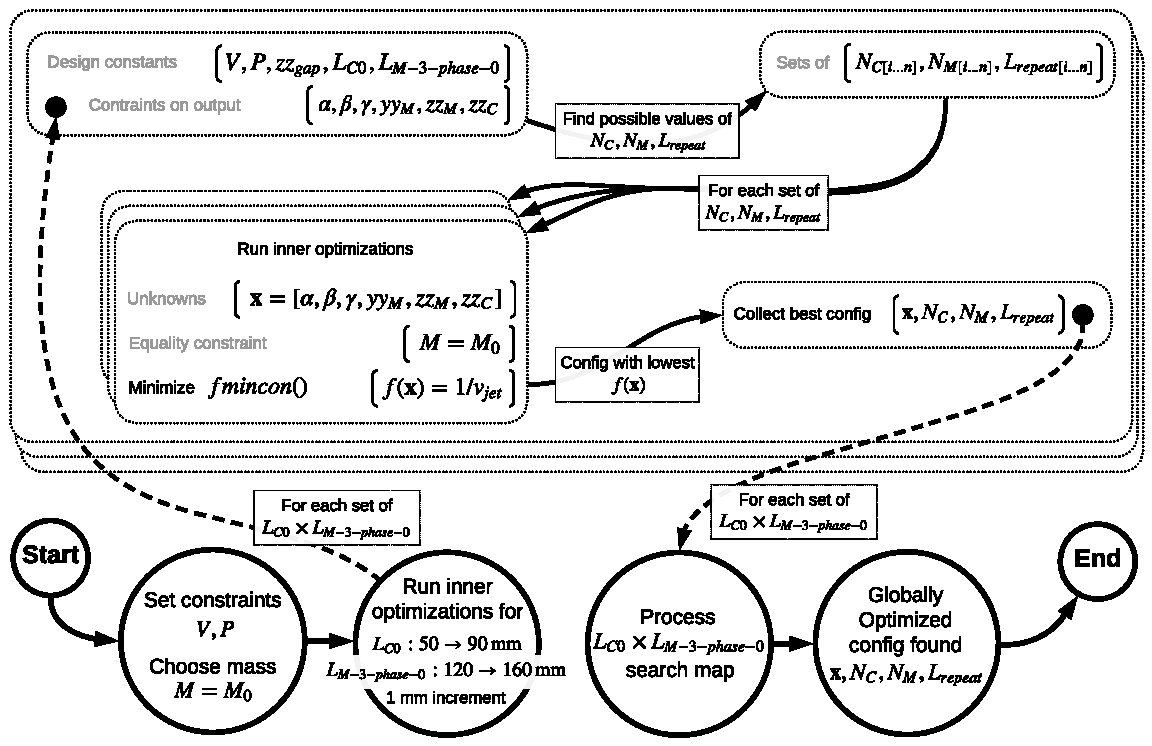
\includegraphics[width=5.9in]{chap4/images3/RSM_LTFM_optimization.pdf}
                  \caption{Summary of the top-level motor optimization algorithm and inner optimization routine for \acsp{LTFM}. The algorithm uses motor specifications $V$, $P$, $M$ to determine the motor parameters $\textbf{x}=[\alpha,\beta,\gamma,yy_M,zz_M,zz_C]$ at which the jet speed $v_{jet}$ can be maximized.}
                  \label{fig:chapter/rsm/LTFM/top level optmization}
                \end{figure*}
    
    
                \begin{table}[h]
                    \renewcommand{\arraystretch}{1.2}
                    \caption{Summary of \acs{LTFM} inner and outer optimization constraints}
                    \label{table:chap/rsm/LTFM/inner and outer constraints}
                    \centering
                    \begin{tabular}{@{}llr@{}}
                    \hline
                    \bfseries Parameter & \bfseries Description & \bfseries Values\\
                    \hline
                        $\alpha$	    & Ratio of $xx_M$ over half period length $L_{repeat}/2$  &	$0.3-0.9$\\ 
                        $\beta$	        & Ratio of coil width $yy_C$ over $yy_M$	&	$1.0-3.0$\\ 
                        $\gamma$	    & Ratio of $zz_U$ over coil height	$zz_C$	&	$0.3-0.7$\\ 
                        $L_{repeat}$    & Repeat length unit length                 &   $5-30\,\mathrm{mm}$\\
                        $yy_M$	        & Width of magnet pieces 	                &	$2-12\,\mathrm{mm}$\\ 
                        $zz_M$	        & Height of magnet pieces			        &	$2-12\,\mathrm{mm}$\\ 
                        $zz_C$	        & Height of coil winding block 			    &	$3-12\,\mathrm{mm}$\\ 
                        $zz_{gap}$      & Z direction mover/stator gap              &	$1.2\,\mathrm{mm}$\\ 
                        \hline
                        $N_C$	        & Number of armature repeat units 		    &	Equation\,\,\ref{eq:chap/rsm/LTFM/list of N_C} \\ 
                        $N_M$	        & Number of mover repeat units 		        &	Equation\,\,\ref{eq:chap/rsm/LTFM/N_M}\\ 
                        $L_{C0}$	    & Equality constraint on 		            &	$50-90\,\mathrm{mm}$\\ 
                                        & \quad the length of a single-phase armature       &   \\
                        $L_{M-3-phase-0}$	    & Inequality constraint on the length of stator &	$120-160\,\mathrm{mm}$\\
                    \hline
                    \end{tabular}
                \end{table}
    
    
                In the wider perspective, the outer optimization loop provided unique combinations of $L_{C0}$, $L_{M-3-phase-0}$ and $M_0$ to provide a set of possible $N_C$, as well as the corresponding values of $N_M$ and $L_{repeat}$. For a particular mass constraint $M_0$ and each point in the $L_{C0}\times L_{M-3-phase-0}$ space, multiple inner most optimizations conducted non-linear constraint optimizations for the unknown variables vector $\textbf{x}$:
                
                
                \begin{equation}
                    \textbf{x} = \big[ \alpha,\beta,\gamma, yy_M, zz_M, zz_C \big]
                    \label{eq:chap/rsm/LTFM/optimization output}
                \end{equation}
                
                
                The aim for each inner optimizations was to find $\textbf{x}$ with the given $[N_C,N_M,L_{repeat},M_0]$ from the outer optimization and constants $[P=1.5\,\mathrm{kW},V=1\,\mathrm{mL}]$ to maximize the jet speed $v_{jet}$ achieved. The same variables ranges in Table\,\ref{table:chap/rsm/LTFM/inner and outer constraints} also applied. 
                
                
                From the \acs{ANN} models already trained, the computation resource can readily predict the thrust output of 3-phase \acsp{LTFM} provided the current density at a high accuracy. To predict the thrust output based on the power input, the \acs{ANN} model server automatically interpolated the 3-phase thrust given current density $F(J)$ to extrapolate the thrust produced at the fixed input power $P=1.5\,\mathrm{kW}$ as $F(P)$.
                
                
                The inner optimization used constrained nonlinear multi-variable optimization based on the interior point algorithm (MATLAB Optimization Toolbox) to maximize $v_{jet}$ (Equation\,\ref{eq:v_jet for FSM}). Upon finishing the inner optimization for each pair $L_{C0}\times L_{M-3-phase-0}$, the control flow saved the best performing motor configuration and moved on to the next $L_{C0}\times L_{M-3-phase-0}$ pair. The optimization steps are summarized in Fig.\,\ref{fig:chapter/rsm/LTFM/top level optmization}. The mass term $M$ which accounts for all 3 phases of the motor is obtained via the following set of equations:
                
                
                    \begin{equation}
                        xx_M = \frac{L_{repeat}}{\alpha}
                        \label{eq:chap/rsm/LTFM/mass/xx_m}
                    \end{equation}
                    
                    
                    \begin{equation}
                        yy_B = yy_U = yy_C + 2\,yy_M
                        \label{eq:chap/rsm/LTFM/mass/yyb is yyu}
                    \end{equation}
                
                
                    \begin{equation}
                        V_{unit-back-SMC} = xx_B\,yy_B\,zz_B
                        \label{eq:chap/rsm/LTFM/mass/V unit back smc}
                    \end{equation}
                    
                    
                    \begin{equation}
                        M_{unit-back-SMC} =  V_{unit-back-SMC} \rho_{smc}
                        \label{eq:chap/rsm/LTFM/mass/M unit back smc}
                    \end{equation}


                    \begin{equation}
                        V_{unit-magnets} = 4\,xx_M\,yy_M\,zz_M
                        \label{eq:chap/rsm/LTFM/mass/V unit 4 magnets}
                    \end{equation}
                    
                    
                    \begin{equation}
                        M_{unit-magnets} =  V_{unit-magnets}\,\rho_{m}
                        \label{eq:chap/rsm/LTFM/mass/M unit 4 magnets}
                    \end{equation}
                    
                    
                    \begin{equation}
                        V_{unit-winding} = 2\,xx_C\,yy_C\,zz_C
                        \label{eq:chap/rsm/LTFM/mass/V unit windings}
                    \end{equation}
                    
                    
                    \begin{equation}
                        M_{unit-winding} =  V_{unit-winding} \big( 0.6\,\rho_{c} + 0.4\,\rho_{ins} \big)
                        \label{eq:chap/rsm/LTFM/mass/M unit windings}
                    \end{equation}
                    
                    
                    \begin{equation}
                        V_{unit-U-core} = xx_U\,yy_U\,zz_U - xx_U\,yy_C,\,zz_C
                        \label{eq:chap/rsm/LTFM/mass/V unit U-core smc}
                    \end{equation}
                    
                    
                    \begin{equation}
                        M_{unit-U-core} =  V_{unit-U-core}\,\rho_{smc}
                        \label{eq:chap/rsm/LTFM/mass/M unit U-core smc}
                    \end{equation}
                    
                    
                    \begin{equation}
                        M_{unit-mover} =  M_{unit-winding}+M_{unit-U-core}
                        \label{eq:chap/rsm/LTFM/mass/M unit mover}
                    \end{equation}
                    
                    
                    \begin{equation}
                        M_{unit-stator} =  M_{unit-magnets}+M_{unit-back-SMC}
                        \label{eq:chap/rsm/LTFM/mass/M unit stator}
                    \end{equation}
                    
                    
                    \begin{equation}
                        M =  3 \big( M_{unit-mover}\,N_C + M_{unit-stator}\,N_M \big)
                        \label{eq:chap/rsm/LTFM/mass/total mass}
                    \end{equation}
                    
                    
                where the assumed copper fill factor is $60\%$, and material densities $\rho_{smc}$, $\rho_c$, $\rho_{ins}$, $\rho_{m}$ are $7500\,\mathrm{kg/m^3}$, $8920\,\mathrm{kg/m^3}$, $1350\,\mathrm{kg/m^3}$, $7600\,\mathrm{kg/m^3}$, respectively.

        % -----------------------------------------------------------------------------------
        % --- NEW SUB SECTION --- NEW SUB SECTION --- NEW SUB SECTION --- NEW SUB SECTION --- 
        % -----------------------------------------------------------------------------------
        \subsection{Results}                   \label{Chapter:RSM/LTFM/Results}
        
            
            With the objective function evaluation using \acs{ANN} models and the conversion engine that translate from thrust given current density $F(J)$ to thrust given power $F(P)$ at its core, the global optimization results of \acs{LFSM} was collected and summarized in Table\,\ref{table:chap/rsm/LFSM/result for global optimization of LTFM via RSM method}. The table shows the optimization results for different motor mass constraints $M0 = [325, 350, 375, 400, 425]\,\mathrm{g}$.
            
            
            Looking at one specific result for the global optimization of constraints set $P=1500\,\mathrm{W}$, $V=1\,\mathrm{mL}$, $zz_{gap}=1.2\,\mathrm{mm}$, $M_0=325\,\mathrm{g}$ on the search space $L_{C0}:50-90\,\mathrm{mm}$, and $L_{M-3-phase-0}:120-160\,\mathrm{mm}$, the result is an under-hung \acs{LTFM} with $\alpha=0.90$, $\beta=1.75$, $\gamma=0.59$, $yy_M=3.15\,\mathrm{mm}$, $zz_M=2\,\mathrm{mm}$, $zz_C=4.16\,\mathrm{mm}$, $L_{repeat}=12.5\,\mathrm{mm}$, $N_C=4$, $N_M=12$, $L_C=50\,\mathrm{mm}$, $L_M=150\,\mathrm{mm}$, $L_{M-3-phase}=158.33\,\mathrm{mm}$ and $L_{stroke}=100\,\mathrm{mm}$. The motor is able to produce $\overline{F} = 145\,\mathrm{N}$ and average jet speed $\overline{v_{jet}}=170.3\,\mathrm{m/s}$. The achievable jet speed is not far from $200\,\mathrm{m/s}$, the jet speed required to guarantee a \acs{NFJI} delivery. 
            
            
            If we now adjust the radius of the drug ampoule so that the average jet speed can reach $200\,\mathrm{m/s}$, the maximum drug volume $V$ that can be delivered is now $V_{new}=0.72\,\mathrm{mL}$. This conversion was explained in Equation\,\ref{eq:v_jet and V} and \ref{eq:v_jet and V ratio}. For the optimized motor configurations obtained at mass $M$ of $350\,\mathrm{g}$, $375\,\mathrm{g}$, $400\,\mathrm{g}$, $425\,\mathrm{g}$, the corresponding average jet speed $\overline{v_{jet}}$ are $177.58\,\mathrm{m/s}$, $183.23\,\mathrm{m/s}$, $189.19\,\mathrm{m/s}$, $197.35\,\mathrm{m/s}$, respectively. The reduced volumes $V_{new}$ for these motors are $0.79\,\mathrm{mL}$, $0.84\,\mathrm{mL}$, $0.89\,\mathrm{mL}$, and $0.97\,\mathrm{mL}$, in the same order. Fig.\,\ref{fig:chapter/rsm/LTFM/optimization search space result for differnt mass} provides global optimization plots of $\overline{v_{jet}}$ for the search space $L_{M-3-phase-0}:120\,\mathrm{mm}\rightarrow 160\,\mathrm{mm} \times L_{C0}:50\,\mathrm{mm}\rightarrow 90\,\mathrm{mm}$ using $P=1500\,\mathrm{W}$, $V=1\,\mathrm{mL}$, $zz_{gap}=1.2\,\mathrm{mm}$ and $M_0=[325,350,375,400,425]\,\mathrm{g}$. 
        
        
            \begin{landscape}
                \begin{table}
                    \renewcommand{\arraystretch}{1.2}
                    \caption{Summary of \acs{LTFM} design optimization values and performance using \acs{RSM} method}
                    \label{table:chap/rsm/LFSM/result for global optimization of LTFM via RSM method}
                    \centering
                    \begin{tabular}{lllrrrrr}
                        \hline
                            \textbf{Params}     & \textbf{Description}                            & \textbf{Unit}           & $M_0=\mathbf{325\,g}$ & $\mathbf{350\,g}$ & $\mathbf{375\,g}$ & $\mathbf{400\,g}$ & $\mathbf{425\,g}$ \\
                        \hline
                            $P$                     & Fixed electrical power input                         & $\mathrm{kW}$  & 1.50   & 1.50   & 1.50   & 1.50   & 1.50   \\
                            $V$                     & Volume of \acs{NFJI} drug ampoule                    & $\mathrm{mL}$  & 1.00   & 1.00   & 1.00   & 1.00   & 1.00   \\
                            $zz_{gap}$              & Mover and stator gap                                 & $\mathrm{mm}$  & 1.20   & 1.20   & 1.20   & 1.20   & 1.20   \\
                        \hline
                            $L_{C0:optim}$          & Inner loop's $L_C$ at global optimum                 & $\mathrm{mm}$  & 50.00  & 50.00  & 50.00  & 50.00  & 50.00  \\
                            $L_{M-3-phase-0:optim}$ & Inner loop's $L_{M-3-phase-0}$ at global optimum     & $\mathrm{mm}$  & 160.00 & 159.00 & 159.00 & 160.00 & 160.00 \\
                        \hline
                            $\alpha$                & Ratio of $w_M$ over $L_{KC}$                         &                & 0.90   & 0.90   & 0.90   & 0.90   & 0.90   \\
                            $\beta$                 & Ratio of $w_C$ over $w_S$                            &                & 1.75   & 1.67   & 1.74   & 1.58   & 1.31   \\
                            $\gamma$                & Ratio of $h_{CM}$ over $h_C$                         &                & 0.59   & 0.59   & 0.56   & 0.57   & 0.58   \\
                            $yy_M$                  & Width of magnet pieces                               & $\mathrm{mm}$  & 3.15   & 3.28   & 3.48   & 3.66   & 3.87   \\
                            $zz_M$                  & Height of magnet pieces                              & $\mathrm{mm}$  & 2.00   & 2.00   & 2.00   & 2.00   & 2.00   \\
                            $zz_C$                  & Height of coil winding block                         & $\mathrm{mm}$  & 4.16   & 4.59   & 4.18   & 4.60   & 5.20   \\
                        \hline
                            $L_{repeat}$             & Repeat length unit length                            & $\mathrm{mm}$  & 12.50  & 12.50  & 12.50  & 12.50  & 12.50  \\
                            $N_C$                   & Number of armature repeat units                      &                & 4      & 4      & 4      & 4      & 4      \\
                            $N_M$                   & Number of mover repeat units                         &                & 12     & 12     & 12     & 12     & 12     \\
                            $L_C$                   & Total length of armature in a single phase           & $\mathrm{mm}$  & 50.00  & 50.00  & 50.00  & 50.00  & 50.00  \\
                            $L_M$                   & Total length of secondary in a single phase          & $\mathrm{mm}$  & 150.00 & 150.00 & 150.00 & 150.00 & 150.00 \\
                            $L_{M-3-phase}$         & Total length of the 3-phase motor                    & $\mathrm{mm}$  & 158.33 & 158.33 & 158.33 & 158.33 & 158.33 \\
                            $L_{stroke}$            & Real stroke length                                   & $\mathrm{m/s}$ & 100.00 & 100.00 & 100.00 & 100.00 & 100.00 \\
                        \hline
                            $\overline{v_{jet}}$    & Average jet speed predicted                          & $\mathrm{m/s}$ & 170.30 & 177.58 & 183.23 & 189.19 & 197.35 \\
                            $\overline{F}$          & Average thrust predicted by the \acs{ANN}            & $\mathrm{N}$   & 145.00 & 157.67 & 167.86 & 178.96 & 194.73 \\
                        \hline
                    \end{tabular}
                \end{table}
            \end{landscape}
                
                
            \begin{figure*}[!ht]
                \centering
                \subfloat[$M_0=325\,\mathrm{g}$. Global optimum found at $L_{C0}=50\,\mathrm{mm}$, and $L_{M-3-phase-0}=160\,\mathrm{mm}$.
                ]{
                    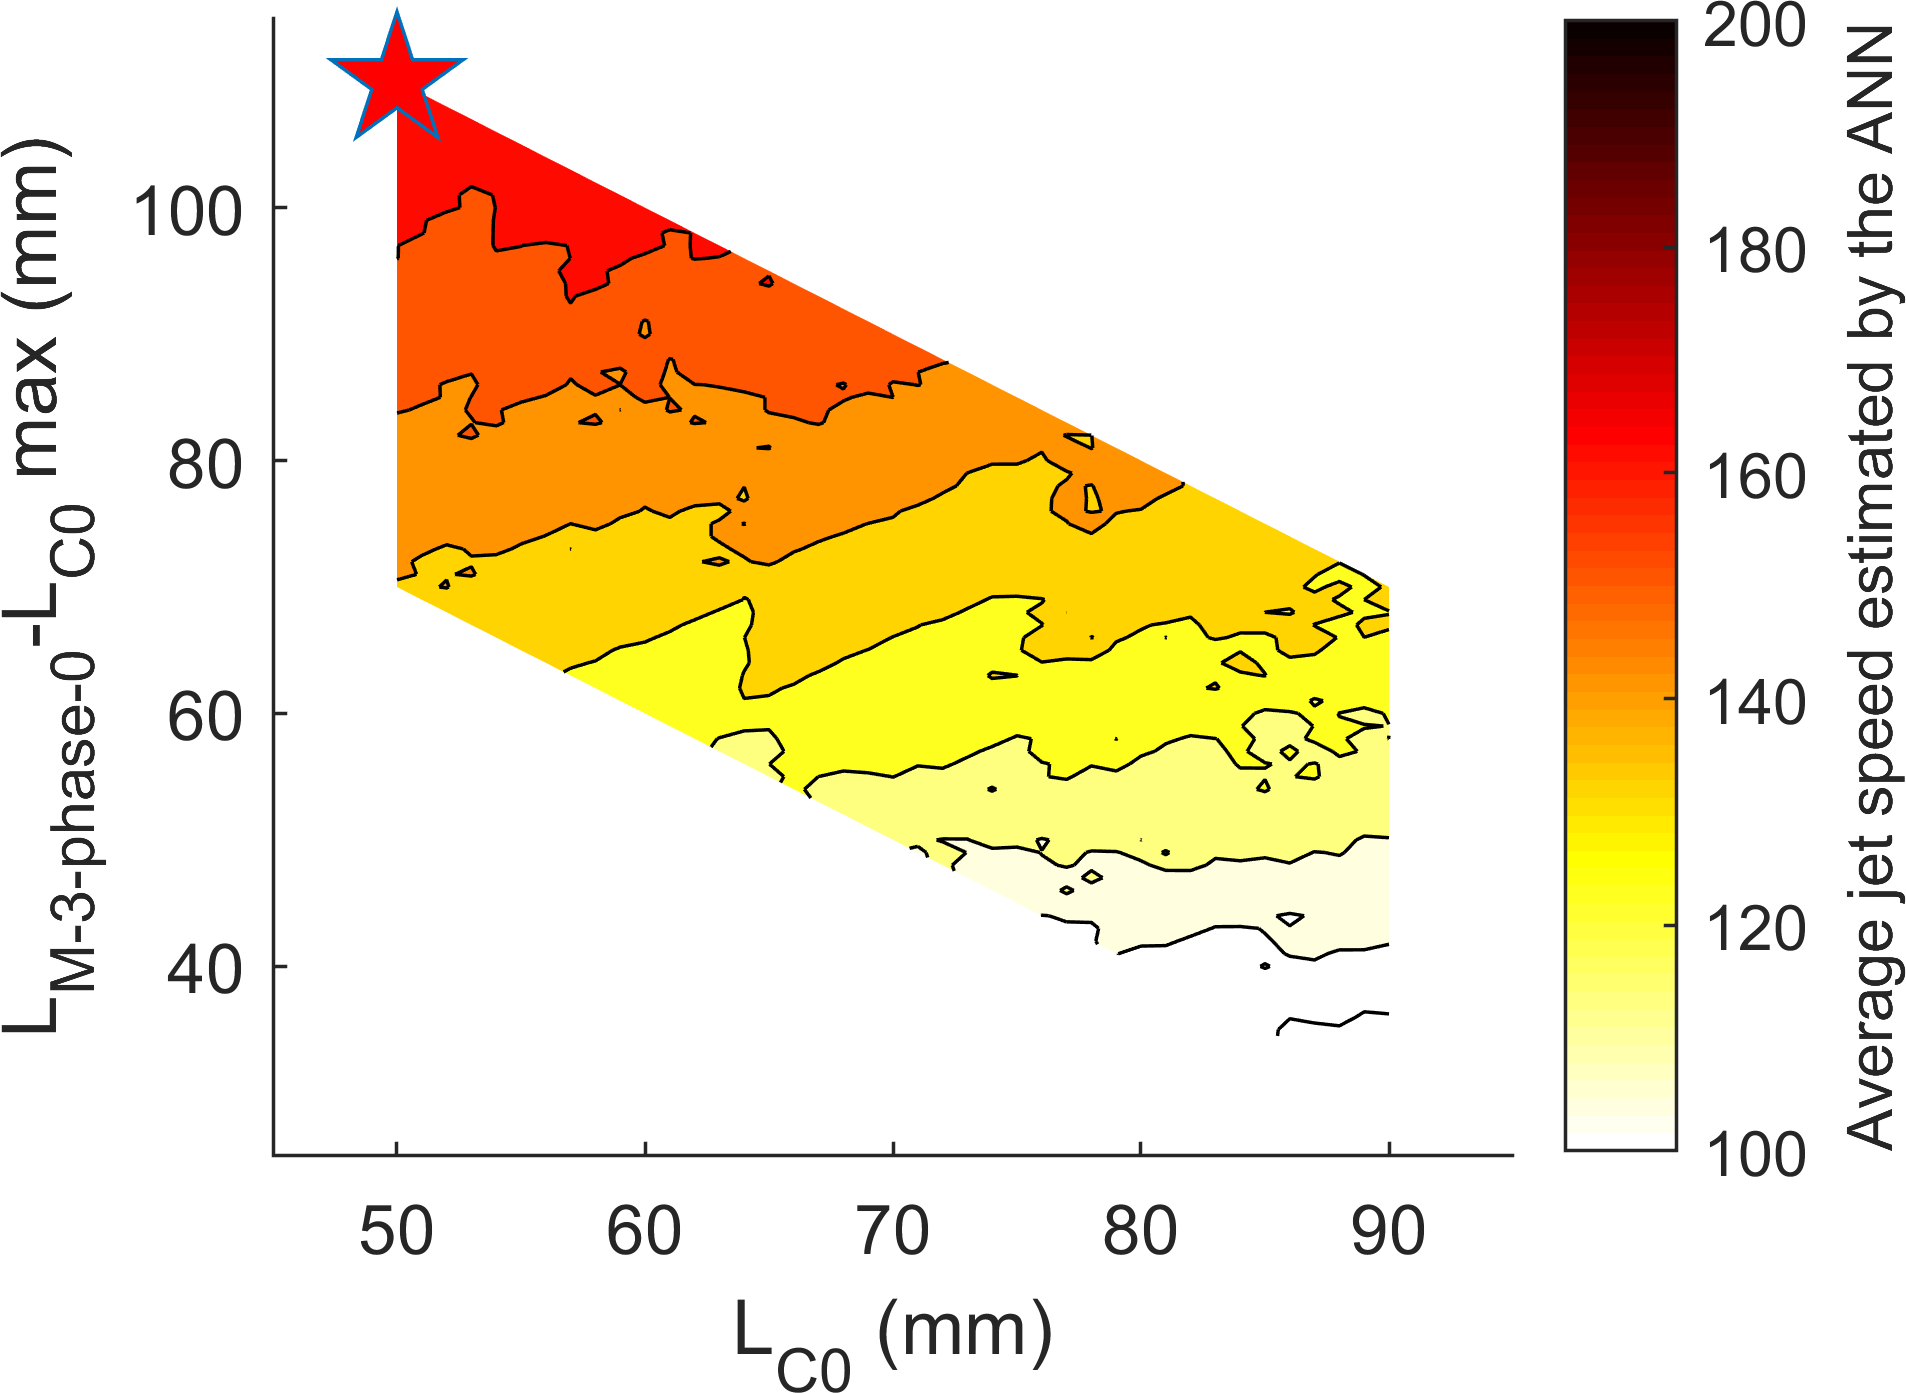
\includegraphics[width=0.45\textwidth]{chap4/images3/325g.png}
                    \label{fig:chapter/rsm/LTFM/optimization/325}
                }
                \qquad
                \subfloat[$M_0=350\,\mathrm{g}$. Global optimum found at $L_{C0}=50\,\mathrm{mm}$, and $L_{M-3-phase-0}=159\,\mathrm{mm}$.
                ]{
                    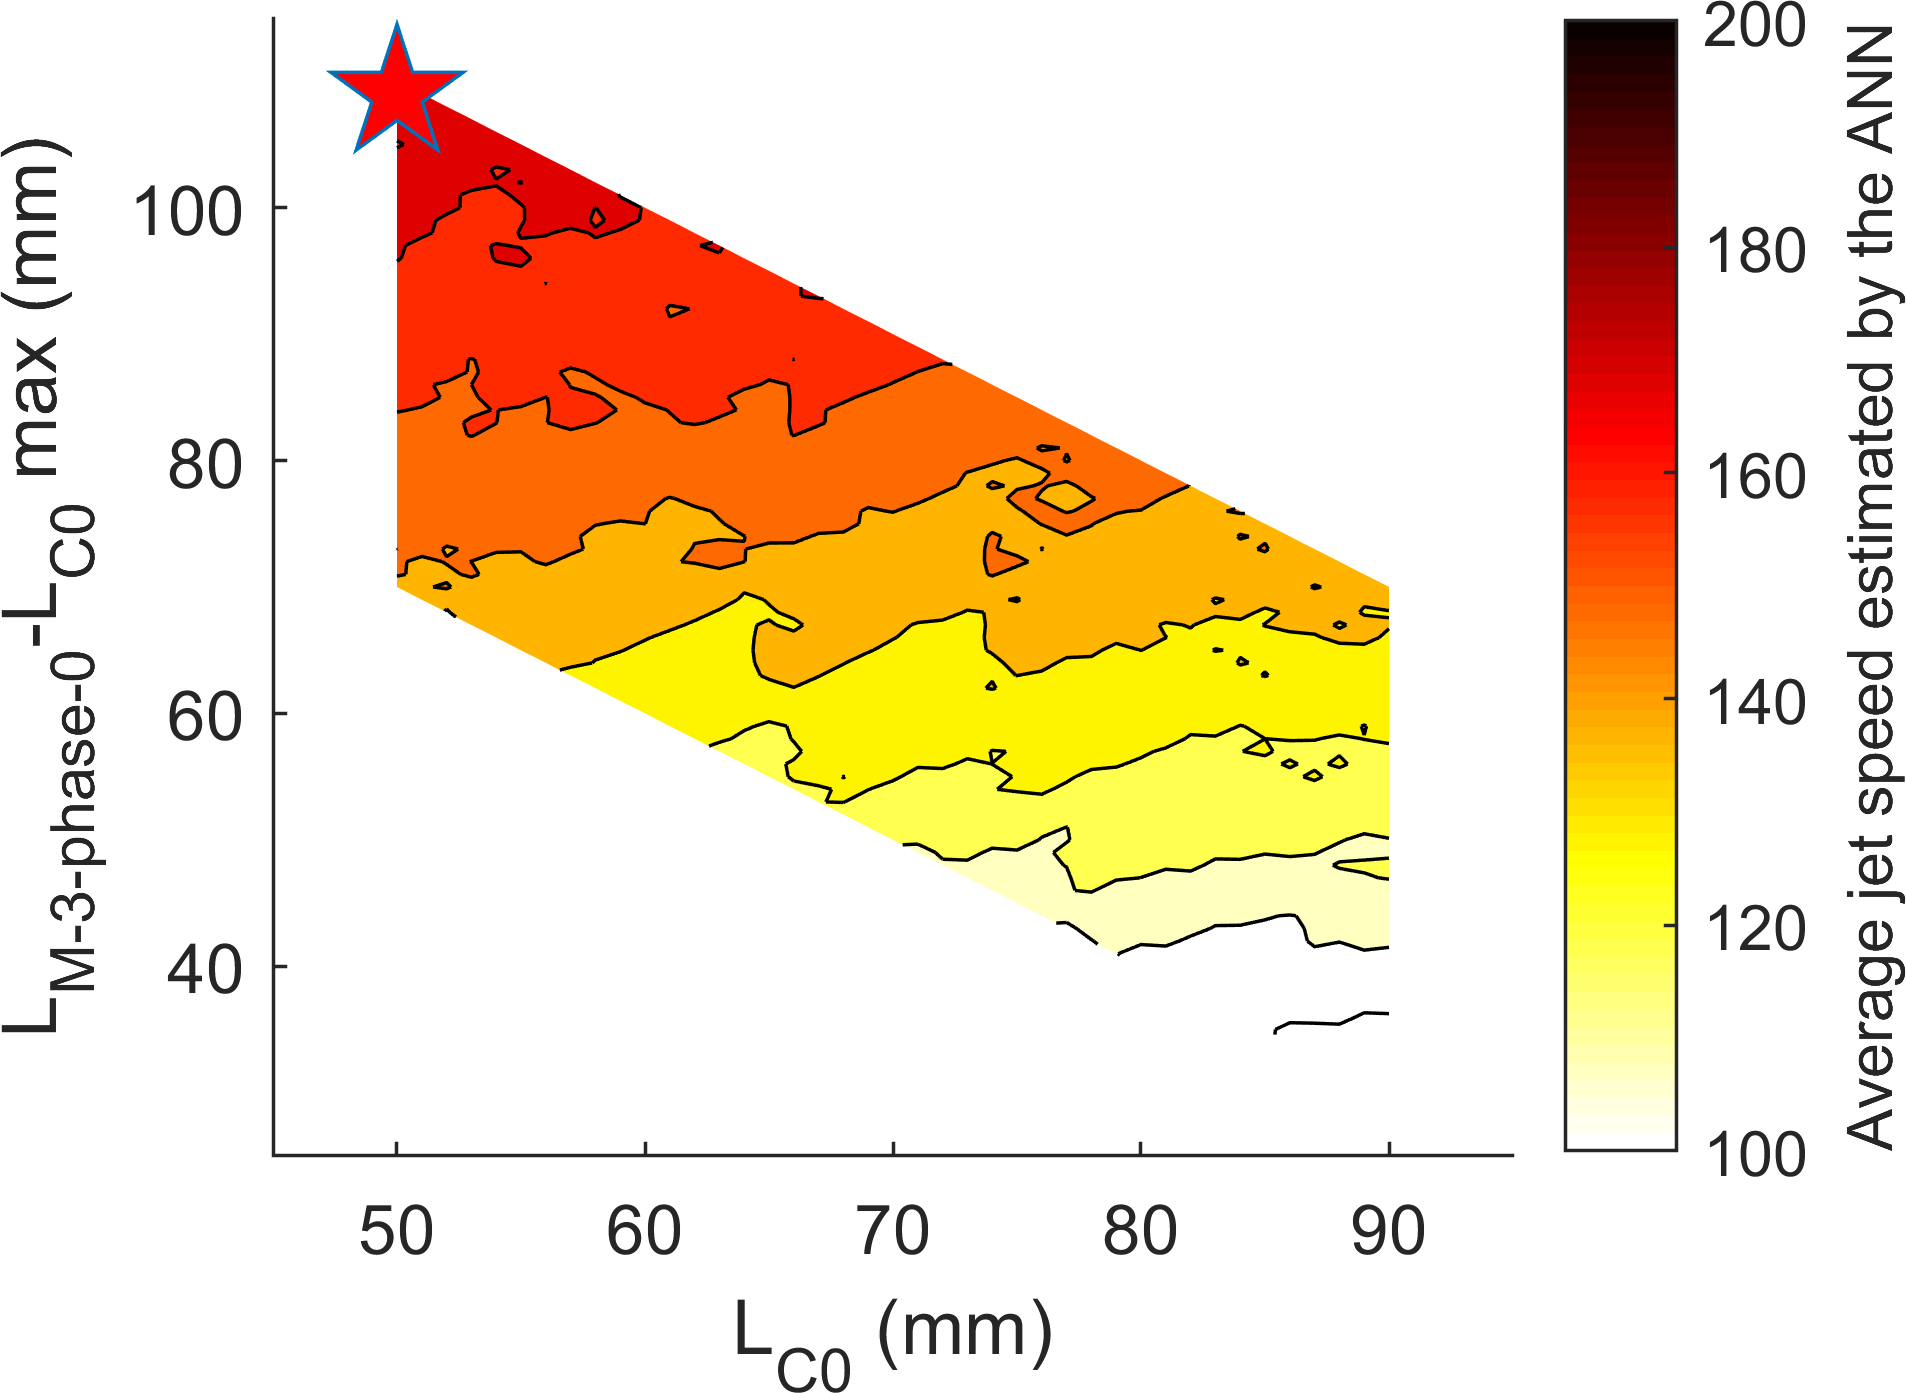
\includegraphics[width=0.45\textwidth]{chap4/images3/350g.png}
                    \label{fig:chapter/rsm/LTFM/optimization/350}
                }
                \\
                \subfloat[$M_0=375\,\mathrm{g}$. Global optimum found at $L_{C0}=50\,\mathrm{mm}$, and $L_{M-3-phase-0}=160\,\mathrm{mm}$.
                ]{
                    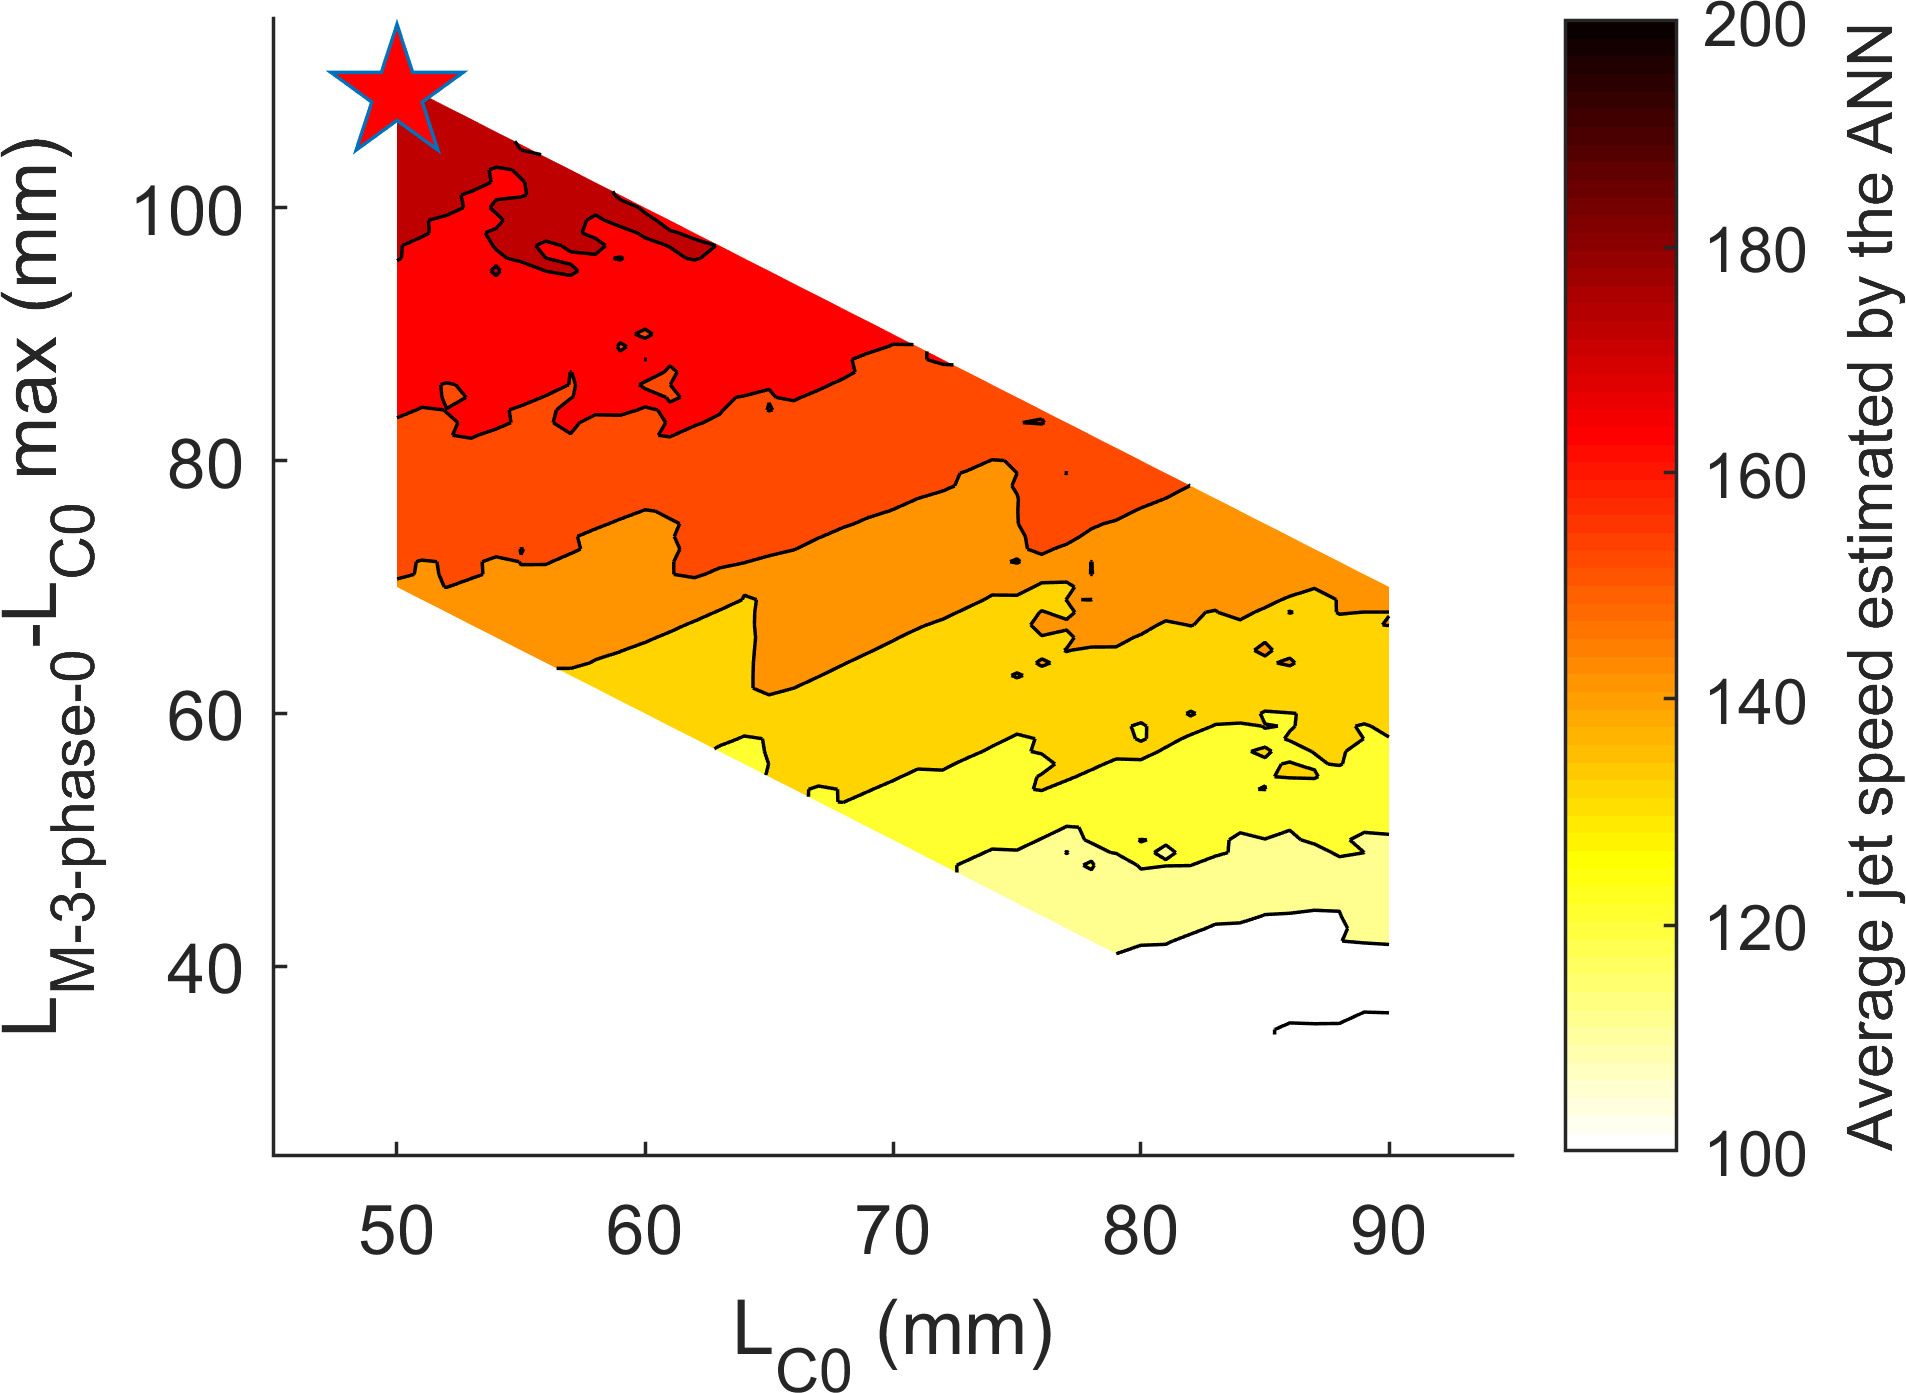
\includegraphics[width=0.45\textwidth]{chap4/images3/375g.png}
                    \label{fig:chapter/rsm/LTFM/optimization/375}
                }
                \qquad
                \subfloat[$M_0=400\,\mathrm{g}$. Global optimum found at $L_{C0}=50\,\mathrm{mm}$, and $L_{M-3-phase-0}=160\,\mathrm{mm}$.
                ]{
                    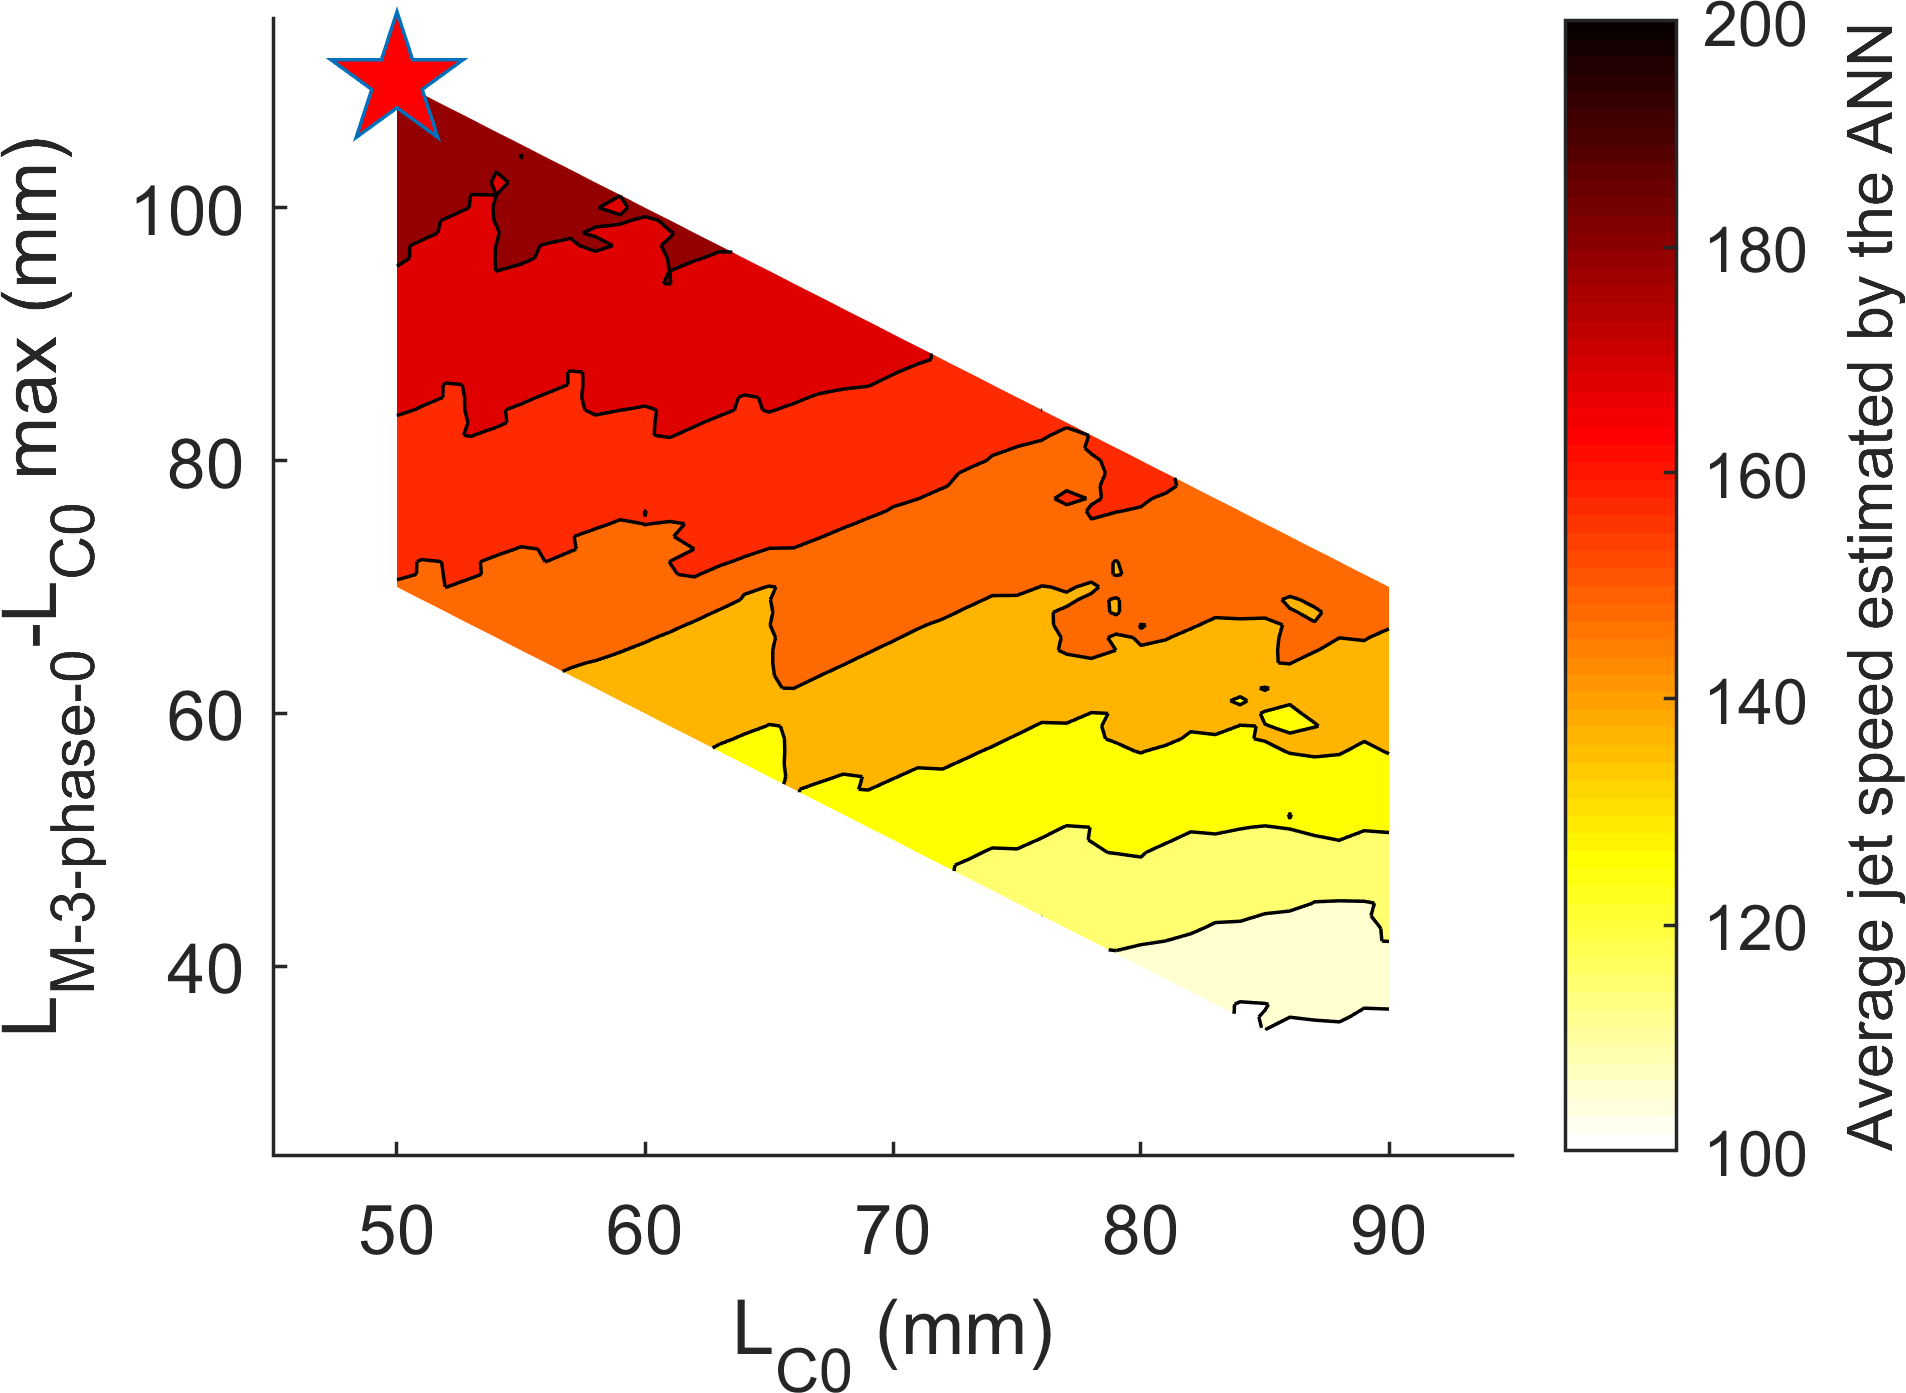
\includegraphics[width=0.45\textwidth]{chap4/images3/400g.png}
                    \label{fig:chapter/rsm/LTFM/optimization/400}
                }
                \\
                \subfloat[$M_0=425\,\mathrm{g}$. Global optimum found at $L_{C0}=50\,\mathrm{mm}$, and $L_{M-3-phase-0}=160\,\mathrm{mm}$.
                ]{
                    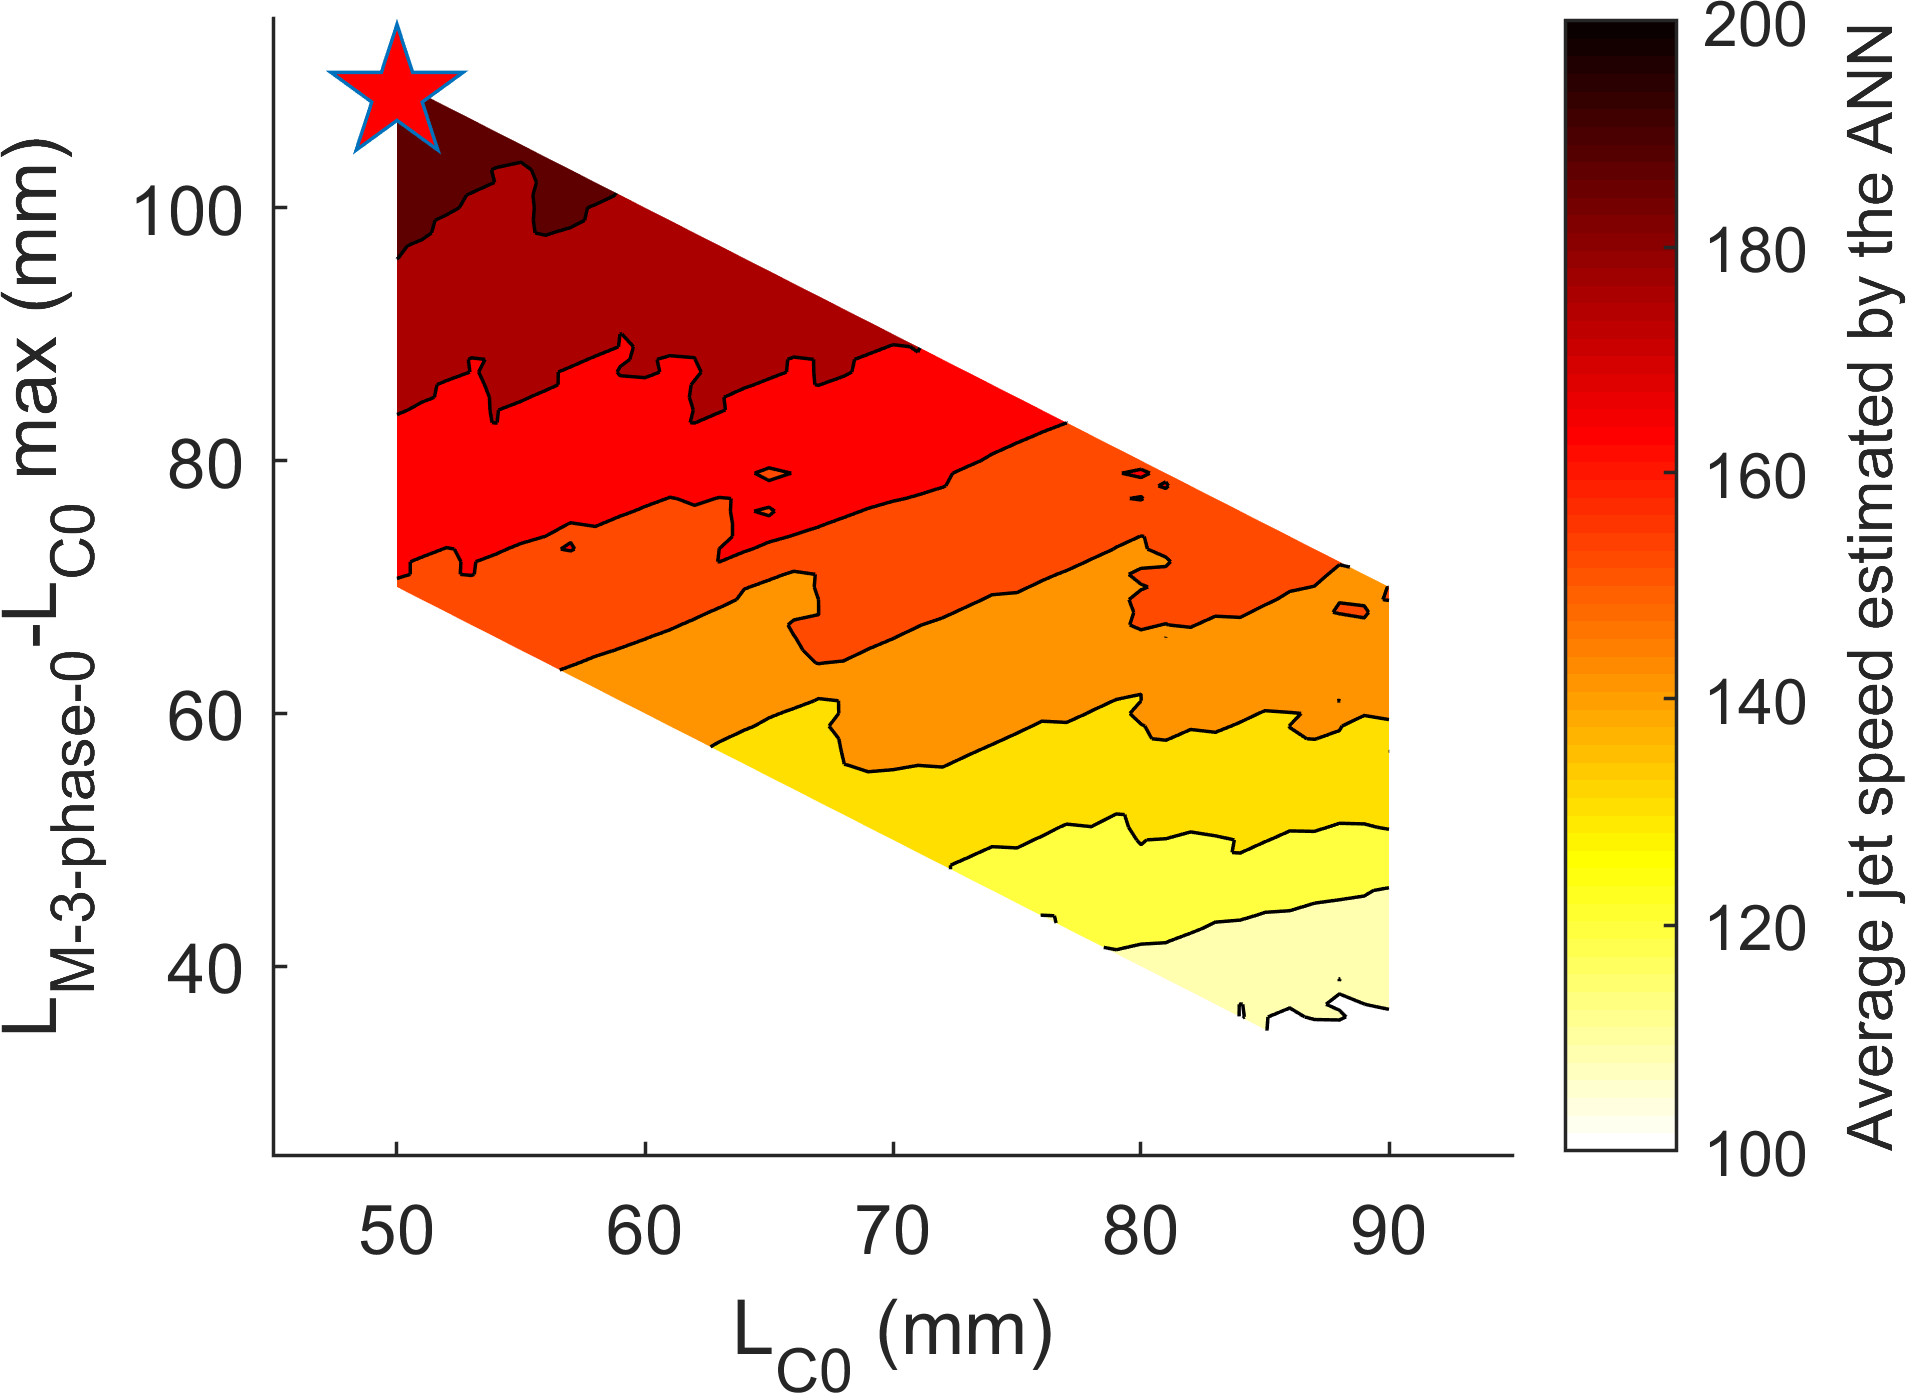
\includegraphics[width=0.45\textwidth]{chap4/images3/425g.png}
                    \label{fig:chapter/rsm/LTFM/optimization/425}
                }
                \\
                \caption{
                    The global optimization plots of $v_{jet}$ for the search space $L_{M-3-phase-0}:120\,\mathrm{mm}\rightarrow 160\,\mathrm{mm} \times L_{C0}:50\,\mathrm{mm}\rightarrow 90\,\mathrm{mm}$ using $P=1500\,\mathrm{W}$, $V=1\,\mathrm{mL}$, $zz_{gap}=1.2\,\mathrm{mm}$,  and $M_0$ of: (a) $325\,\mathrm{g}$, (b) $350\,\mathrm{g}$, (c) $375\,\mathrm{g}$, (d) $400\,\mathrm{g}$, and (e) $425\,\mathrm{g}$.
                }   \label{fig:chapter/rsm/LTFM/optimization search space result for differnt mass}
            \end{figure*}
            
            

            
    
    % ===================================================================================================
    % === NEW SECTION === NEW SECTION === NEW SECTION === NEW SECTION === NEW SECTION === NEW SECTION ===
    % ===================================================================================================
    \section{Discussion}                            \label{Chapter:RSM/discussion}
    
    
        In this chapter, \acf{PMLSM}, \acf{LFSM}, \acf{LTFM} have been analyzed, investigated and optimized for \acf{NFJI} application with a common objective and set of constraints outlined earlier in Equation\,\ref{eq:outer optimization for PMLSMs}. The underlying method was a robust process of studying each types of motor in depth, making thoughtful assumptions that reduce the difficulties in modelling, mining the valuable design library with the available \acf{HPC} resource, applying advanced machine techniques to build highly accurate \acf{ANN} models, and efficiently conducting reproducible optimization studies. The advantage of the \acf{RSM} process generally applied in this chapter is flexibility. It could be used to study and optimize types of motors that the literature has little success in analytical modelling, for potentially a wide range of applications. This process includes a rather lengthy data collection process, however, once the data is collected, that same set of data could be utilized in multiple different ways and applications.
        
        
        Table\,\ref{table:chap/rsm/overall optimization results} summarized important design characteristic and the performance of each types of motor at different mass constraints. The average thrust, the average jet speed, and the equivalent delivery volume data comparison concluded that \acs{PMLSM} significantly out-perform \acs{LFSM}, and \acs{LTFM} for the given \acs{NFJI} task. Therefore, \acs{PMLSM} is selected to be further studied, optimized and constructed for \acs{NFJI}. 
        
        
        As opposed to the the literature belief, \acs{LTFM} was perceived to perform more poorly than the \acs{PMLSM} in this  particular \acs{NFJI} application. This may be representative for the U-core \acs{LTFM} structure but not all \acs{LTFM} topologies. Future work should certainly explore other \acs{LTFM} topologies.
   
        
        \begin{landscape}
            \begin{table}[]
                \renewcommand{\arraystretch}{1.2}
                \caption{Summary of design optimization results for PMLSM, LFSM, and LTFM}
                \label{table:chap/rsm/overall optimization results}
                \begin{tabular}{l|rrr|rrr|rrr|r}
                \hline
                \multicolumn{1}{l|}{$\textbf{Types of motors}$}                         & \multicolumn{3}{c|}{$\textbf{PMLSM}$}            & \multicolumn{3}{c|}{$\textbf{LFSM}$}             & \multicolumn{3}{c|}{$\textbf{LTFM}$}             &  {$\textbf{Units}$}              \\ 
                \hline
                Mass Constraints $M_0$                                       & $\textbf{325}$ & $\textbf{375}$ & $\textbf{425}$ & $\textbf{325}$ & $\textbf{375}$ & $\textbf{425}$ & $\textbf{325}$ & $\textbf{375}$ & $\textbf{425}$ & $\mathrm{g}$   \\
                Armature repeats $N_C$                                       & 4              & 3              & 3              & 6              & 6              & 6              & 4              & 4              & 4              &                \\
                Secondary repeats $N_S$ or $N_M$                             & 12             & 9              & 9              & 17             & 16             & 16             & 12             & 12             & 12             &                \\
                Repeat length $L_k$ or $L_{repeat}$                          & 26.5           & 35.3           & 35.3           & 65             & 70             & 70             & 12.5           & 12.5           & 12.5           & \multicolumn{1}{r}{$\mathrm{mm}$} \\
                Length of mover $L_C$                                        & 53             & 53             & 53             & 65             & 70             & 160            & 50             & 50             & 50             & \multicolumn{1}{r}{$\mathrm{mm}$} \\
                Length of stator $L_M$ or $L_S$                              & 159            & 169            & 159            & 157.9          & 160            & 160            & 158.3          & 158.3          & 158.3          & \multicolumn{1}{r}{$\mathrm{mm}$} \\
                Stroke length $L_{stroke}$ or length of ampoule              & 106            & 106            & 106            & 93             & 90             & 90             & 100            & 100            & 100            & $\mathrm{mm}$  \\
                \hline
                Average thrust $\overline{F}$ at $V=1\,\mathrm{mL}$          & 246            & 271            & 283            & 129            & 149            & 165            & 145            & 168            & 195            & $\mathrm{N}$   \\
                Average jet speed $\overline{v_{jet}}$ at $V=1\,\mathrm{mL}$ & 229            & 240            & 250            & 155            & 164            & 172            & 170            & 183            & 197            & $\mathrm{m/s}$ \\
                Equivalent $V$ at $\overline{v_{jet}}=200\,\mathrm{m/s}$     & 1.31           & 1.43           & 1.56           & 0.60           & 0.67           & 0.74           & 0.72           & 0.84           & 0.97           & $\mathrm{mL}$ \\
                \hline
                \end{tabular}
            \end{table}
        \end{landscape}